\documentclass[a4paper,10pt,titlepage,oneside,openany]{book}

% ===== Packages =====
\usepackage[skip=6pt]{parskip}
\usepackage[english]{babel}
\usepackage[utf8]{inputenc}
\usepackage[T1]{fontenc}
\usepackage{graphicx}
\usepackage{amsmath,amssymb,amsthm}
\usepackage{enumitem}
\usepackage{float}
\usepackage{changepage}
\usepackage[top=1in, bottom=1in, left=1in, right=1in]{geometry}
\usepackage{fancyhdr}
\usepackage{tcolorbox}
\usepackage{array}
\usepackage{booktabs}
\usepackage{tabularx}
\usepackage{pdfpages}
\usepackage[hypertexnames=false,colorlinks=true, linkcolor=black, citecolor=black, urlcolor=blue]{hyperref}
\usepackage{etoolbox}
\usepackage{ragged2e}
\usepackage{mathtools}
\usepackage{caption}
\usepackage{subcaption}
\usepackage[ruled,vlined]{algorithm2e}
\usepackage{listings}
\usepackage{xcolor}

% ===== Default layout =====
\AtBeginDocument{\justifying}
\setlength{\parindent}{0pt}
\setlength{\parskip}{6pt}
\graphicspath{{../template/}{template/}{./}}

% ===== Header / Footer =====
\pagestyle{fancy}
\fancyhf{}
\fancyhead[L]{\textbf{Starting Finance Club PoliTo}}
\fancyhead[R]{\IfFileExists{../template/Logo_SFClub_Polito.png}{\includegraphics[width=1cm]{../template/Logo_SFClub_Polito.png}}{\IfFileExists{template/Logo_SFClub_Polito.png}{\includegraphics[width=1cm]{template/Logo_SFClub_Polito.png}}{}}}
\fancyfoot[C]{\thepage}
\renewcommand{\headrulewidth}{0.4pt}
\renewcommand{\footrulewidth}{0.4pt}
\setlength{\headheight}{34pt}
\setlength{\headsep}{24pt}

\fancypagestyle{plain}{%
  \fancyhf{}
  \fancyhead[L]{\textbf{Starting Finance Club PoliTo}}
  \fancyhead[R]{\IfFileExists{../template/Logo_SFClub_Polito.png}{\includegraphics[width=1cm]{../template/Logo_SFClub_Polito.png}}{\IfFileExists{template/Logo_SFClub_Polito.png}{\includegraphics[width=1cm]{template/Logo_SFClub_Polito.png}}{}}}
  \fancyfoot[C]{\thepage}
  \renewcommand{\headrulewidth}{0.4pt}
  \renewcommand{\footrulewidth}{0.4pt}
}

% ===== Theorem-like environments =====
\theoremstyle{plain}
\newtheorem{theorem}{Theorem}[chapter]
\newtheorem{proposition}{Proposition}[chapter]
\theoremstyle{definition}
\newtheorem{definition}{Definition}[chapter]
\newtheorem{notation}{Notation}[chapter]
\theoremstyle{remark}
\newtheorem{remark}{Remark}[chapter]

\newenvironment{pseudocode}{\par\small\ttfamily\begin{adjustwidth}{1em}{1em}}{\end{adjustwidth}\par}

\newenvironment{tightabstract}[1][0.88]{%
  \begin{center}
  \begin{tcolorbox}[title={Abstract}, width=#1\textwidth, left=5mm, right=5mm,
    colback=white, boxrule=0.4pt]
  \small\justifying
}{%
  \end{tcolorbox}
  \end{center}
}

\newcommand{\miniabstract}[1]{%
\vspace{-2pt}
\begin{tcolorbox}[colback=gray!6,colframe=black!15,boxrule=0.3pt,arc=3pt,left=6pt,right=6pt,top=4pt,bottom=4pt]
\textit{Mini-abstract.} #1
\end{tcolorbox}
\vspace{-4pt}
}


\makeatletter
\newenvironment{references}{%
  \chapter*{Bibliography}%
  \addcontentsline{toc}{chapter}{Bibliography}%
  \markboth{Bibliography}{Bibliography}%
  \list{\@biblabel{\@arabic\c@enumiv}}{%
    \settowidth\labelwidth{\@biblabel{99}}%
    \leftmargin\labelwidth
    \advance\leftmargin\labelsep
    \@openbib@code
    \usecounter{enumiv}%
    \let\p@enumiv\@empty
    \renewcommand\theenumiv{\@arabic\c@enumiv}}%
  \sloppy
  \clubpenalty4000
  \@clubpenalty\clubpenalty
  \widowpenalty4000
  \sfcode`\.\@m
}{%
  \def\@noitemerr{\@latex@warning{Empty `references' environment}}%
  \endlist
}
\makeatother

% ===== Math shortcuts =====
\newcommand{\E}{\mathbb{E}}
\newcommand{\Var}{\operatorname{Var}}
\newcommand{\Cov}{\operatorname{Cov}}
\newcommand{\R}{\mathbb{R}}
\newcommand{\dd}{\,\mathrm{d}}
\newcommand{\1}{\mathbf{1}}
\newcommand{\Texp}{\mathrm{T}}
\newcommand{\argmin}{\operatorname*{arg\,min}}
%\renewcommand{\qedsymbol}{\raisebox{10.6ex}{\(\square\)}}
% ===== Chapter spacing fixes =====
\makeatletter
\patchcmd{\@makechapterhead}{\vspace*{50\p@}}{\vspace*{-18\p@}}{}{}
\patchcmd{\@makeschapterhead}{\vspace*{50\p@}}{\vspace*{-18\p@}}{}{}
\patchcmd{\@makechapterhead}{\huge}{\fontsize{17}{20}\selectfont\bfseries}{}{}
\patchcmd{\@makechapterhead}{\Huge}{\fontsize{20}{24}\selectfont\bfseries}{}{}
\patchcmd{\@makeschapterhead}{\Huge}{\fontsize{20}{24}\selectfont\bfseries}{}{}
\patchcmd{\@makechapterhead}{\vskip 20\p@}{\vskip 6\p@}{}{}
\patchcmd{\@makechapterhead}{\vskip 40\p@}{\vskip 10\p@}{}{}
\patchcmd{\@makeschapterhead}{\vskip 40\p@}{\vskip 10\p@}{}{}
\makeatother

% ===== Listings =====
\lstdefinestyle{python}{
  language=Python,
  basicstyle=\ttfamily\small,
  keywordstyle=\bfseries,
  commentstyle=\itshape,
  stringstyle=\ttfamily,
  showstringspaces=false,
  breaklines=true,
  frame=single,
  numbers=left,
  numberstyle=\tiny,
  xleftmargin=2em,
  framexleftmargin=1.5em,
  tabsize=4
}
\lstset{style=python}

\begin{document}

% --- Cover page PDF, if available ---
\IfFileExists{../template/Copertina_research.pdf}{%
\includepdf[pages=1,fitpaper=true,pagecommand={\thispagestyle{empty}}]{../template/Copertina_research.pdf}
}{\IfFileExists{template/Copertina_research.pdf}{%
\includepdf[pages=1,fitpaper=true,pagecommand={\thispagestyle{empty}}]{template/Copertina_research.pdf}
}{}}

% --- TITLE/CONTACT/ABSTRACT ---
\begin{titlepage}
\thispagestyle{empty}
\vspace*{-1cm}
\begin{center}
\IfFileExists{../template/Logo_SFClub_Polito.png}{\includegraphics[width=3.7cm]{../template/Logo_SFClub_Polito.png}\par}{\IfFileExists{template/Logo_SFClub_Polito.png}{\includegraphics[width=3.7cm]{template/Logo_SFClub_Polito.png}\par}{\vspace*{2cm}}}
\vspace{1cm}
{\LARGE\bfseries High-Frequency Market Making under Avellaneda--Stoikov:\\ Rough Volatility and End-of-Day Inventory Control\par}
\vspace{0.25cm}
{\large Mathematical foundations of fractional Brownian motion, Volterra processes, and Markovian lifting\par}

\vspace{0.8cm}

{\normalsize
\textbf{Authors:}\\[0.3cm]
Salvatore Gabriele Messina\\
Niccol\`o Soriano\\[0.3cm]
\textit{Date:} October 13, 2026\par
}

\vspace*{0.2cm}

{\Large\textbf{Starting Finance Club PoliTo}\par}

\vspace{0.4cm}
\normalsize

\textit{Contact:}\\
\small
LinkedIn: \url{https://www.linkedin.com/company/startingfinance-club-polito}\\
GitHub: \url{https://github.com/StartingFinanceClubPoliTo/Research}\\
Instagram: \url{https://www.instagram.com/sfclubpolito}\\
Website: \url{https://sfclubpolito.it/}

\vspace{1cm}
\begin{tightabstract}
This paper develops the mathematical background needed before implementing rough-volatility dynamics in an Avellaneda--Stoikov market making framework. The first objective is to introduce fractional Brownian motion as the canonical Gaussian model with long memory, highlighting the role of the Hurst parameter and the covariance structure of fractional Gaussian increments. The second objective is to explain why direct simulation methods based on global covariance construction are not the most natural choice when the final application is sequential quoting and inventory control. For this reason, the paper develops a causal Volterra representation, derives its induced covariance by It\^o isometry, and presents a discrete-time scheme that builds the process iteratively from past information only. The third objective is computational: because pure power-law memory is non-Markovian and expensive to simulate, we introduce Markovian lifting, which approximates a rough kernel with a finite mixture of exponentials and transforms the problem into a finite-dimensional system of Ornstein--Uhlenbeck factors. This recovers a tractable state-space representation that is well suited to filtering, simulation, and eventually control. The final sections explain how these constructions motivate rough-volatility price modules, liquidation-aware reservation prices, and end-of-day inventory control in the second HFT project of the Starting Finance Club PoliTo research program.
\end{tightabstract}
\end{center}
\end{titlepage}

% --- Front matter ---
\frontmatter
\clearpage
\pagenumbering{roman}
\setcounter{page}{1}
\begingroup\small\setlength{\parskip}{0pt}\tableofcontents\endgroup
\thispagestyle{plain}

\chapter*{Introduction and Motivation}
\addcontentsline{toc}{chapter}{Introduction and Motivation}
\markboth{Introduction and Motivation}{Introduction and Motivation}
\miniabstract{This article is the mathematical prelude to the second HFT project. Starting from the limitation of the classical Avellaneda--Stoikov benchmark, it builds the route from fractional covariance to causal Volterra dynamics, Markovian lifting, and the numerical rough-volatility HJB that closes the paper.}

The classical Avellaneda--Stoikov framework is attractive because it isolates the economic logic of market making in a transparent way: the dealer faces a trade-off between spread capture and inventory risk, and optimal quotes are built around an inventory-adjusted reservation price \cite{AvellanedaStoikov2008}. In the standard benchmark, the mid-price is usually modeled by a diffusion with independent increments. This is analytically convenient, but it suppresses the persistence and irregularity that are often associated with volatility at very short horizons.

The rough-volatility literature addresses this limitation by replacing smooth or Markovian variance specifications with kernels that create path dependence and short-scale irregularity \cite{GatheralJaissonRosenbaum2018,ElEuchRosenbaum2019}. At the mathematical core of this idea lies fractional Brownian motion and, more generally, a family of Gaussian Volterra processes. These objects are useful because they encode memory through the covariance structure itself.

For the present project, three levels of description are important.

\begin{enumerate}[label=\arabic*.]
    \item A \textbf{global Gaussian level}, where one defines a target covariance and samples directly from it.
    \item A \textbf{causal Volterra level}, where the process is built from past Brownian increments weighted by a kernel.
    \item A \textbf{lifted Markovian level}, where the singular kernel is approximated by a finite exponential mixture and simulation becomes finite-dimensional again.
\end{enumerate}

The first level is ideal for introducing fractional Brownian motion. The second level is conceptually closer to sequential simulation and filtering. The third level is the most attractive when the final application is control, calibration, or fast Monte Carlo inside a market making engine.

\paragraph{Why this matters for HFT.}
In a single-asset Avellaneda--Stoikov setting, the reservation price is shifted away from the mid-price when inventory becomes large. Under constant or classical diffusion volatility, this correction depends on a local variance scale. Once volatility becomes rough, however, the local risk scale is no longer memoryless. The state of the market inherits persistent information from the recent path, and the numerical engine must be able to update that state in a stable and computationally tractable way.

This is exactly why the route
\[
\text{fractional covariance} \quad \longrightarrow \quad \text{Volterra causality} \quad \longrightarrow \quad \text{Markovian lifting}
\]
is not just a mathematical curiosity, but the natural backbone of a rough-volatility market making implementation.

The next chapter begins from the first layer of that route: fractional Brownian motion. Starting there keeps the paper aligned with the first HFT article's progression from market-making motivation to mathematical engine and then to numerical validation.

% --- Main matter ---
\mainmatter
\clearpage
\setcounter{page}{1}

\chapter{Fractional Brownian Motion}
\miniabstract{The introduction framed rough volatility as the missing risk layer in the classical Avellaneda--Stoikov benchmark. This chapter isolates fractional Brownian motion, the centered Gaussian process whose covariance kernel and Hurst parameter encode memory, roughness, and the increment structure needed for simulation.}

\section{Introduction to Markovian Processes and Fractional Brownian Motion}

In stochastic modeling, a fundamental distinction concerns the way in which past information influences future dynamics. In a \textbf{Markovian} framework, the current state of the system is sufficient to describe the probabilistic evolution of the future. Once the present state is known, conditioning on additional information from the remote past does not improve the description of the next transition. In this sense, all relevant historical information is already encoded in the current state.

\begin{definition}[Markov process]
A stochastic process \(\{X_t\}_{t\ge 0}\), adapted to a filtration \(\{\mathcal{F}_t\}_{t\ge 0}\), is said to be \emph{Markovian} if for every \(0\le s<t\) and every measurable set \(A\),
\[
\mathbb{P}(X_t\in A\mid \mathcal{F}_s)
=
\mathbb{P}(X_t\in A\mid X_s).
\]
Equivalently, the conditional law of the future given the whole past depends only on the present state.
\end{definition}

This property is central in many classical stochastic models because it yields a tractable state-space description: one only needs to keep track of the present value \(X_s\), rather than the whole trajectory up to time \(s\).

Fractional Brownian motion departs from this paradigm. Its defining feature is that past increments remain informative about future behavior even over long horizons. As a result, conditioning on the present state alone is not enough to characterize the future evolution. This is the essence of its \textbf{non-Markovian} nature and of its long-memory structure.

\begin{definition}[Non-Markovian process]
A stochastic process is said to be \emph{non-Markovian} if the Markov property fails, that is, if there exist times \(s<t\) for which the conditional law of \(X_t\) given the past \(\mathcal{F}_s\) cannot be reduced to a function of the current state \(X_s\) alone.
\end{definition}

From this perspective, fractional Brownian motion should be viewed as a genuinely \textbf{path-dependent} Gaussian process. The filtration \(\mathcal{F}_t\), representing all information generated by the trajectory up to time \(t\), plays a crucial role because the process carries memory of its past increments. This feature is particularly relevant in financial applications, especially in volatility modeling, where empirical data often exhibit dependence structures that are not well captured by classical Markovian diffusions. Although non-Markovian models are typically more demanding from a computational standpoint, they offer a richer framework for describing persistent or rough temporal behavior.

\section{Definition and first properties}

A convenient mathematical entry point to fractional Brownian motion is through its increment process. Rather than starting immediately from the continuous-time covariance kernel, it is useful to first introduce the stationary Gaussian sequence that governs its discrete increments. This sequence is called \emph{fractional Gaussian noise} and represents the fundamental building block of the model.

\begin{definition}[Fractional Gaussian noise]
Let \(H\in(0,1)\). A centered stationary Gaussian sequence
\[
\{X_k\}_{k\in\mathbb{Z}}
\]
is called \emph{fractional Gaussian noise} if its covariance function is
\[
\gamma_H(k)
=
\Cov(X_0,X_k)
=
\frac{1}{2}
\left(
|k+1|^{2H}
-
2|k|^{2H}
+
|k-1|^{2H}
\right),
\qquad k\in\mathbb{Z}.
\]
\end{definition}

The parameter \(H\), called the \emph{Hurst parameter}, governs both the dependence structure of the increments and the roughness of the resulting paths. The benchmark case \(H=\tfrac12\) recovers Gaussian white noise,
\[
\gamma_{1/2}(k)=\delta_{k,0},
\]
so that the increments are uncorrelated and, in the Gaussian setting, independent. When \(H>\tfrac12\), the dependence is predominantly positive and the process is persistent; when \(H<\tfrac12\), the dependence becomes predominantly negative and the process is anti-persistent.

Once the increment sequence has been specified, fractional Brownian motion is obtained by accumulation. On a discrete grid, this means that the process is constructed as the cumulative sum of fractional Gaussian noise.

\begin{definition}[Discrete-time fractional Brownian motion]
Let \(\{X_k\}_{k\ge 1}\) be a fractional Gaussian noise sequence with Hurst parameter \(H\). The associated discrete-time fractional Brownian motion is defined by
\[
B_0^H=0,
\qquad
B_n^H=\sum_{j=1}^{n}X_j,
\qquad n\ge 1.
\]
\end{definition}

Equivalently, on a uniform grid \(t_n=n\Delta t\), one may write
\[
B^H_{t_n}
=
\sum_{j=1}^{n}\Delta B_j^H,
\qquad
\Delta B_j^H:=B^H_{t_j}-B^H_{t_{j-1}},
\]
where, after the appropriate normalization, the increment sequence \(\{\Delta B_j^H\}\) has the covariance structure of fractional Gaussian noise.

The continuous-time version is the canonical Gaussian process associated with this dependence structure.

\begin{definition}[Fractional Brownian motion]
Let \(H\in(0,1)\). A process \(\{B_t^H\}_{t\ge 0}\) is called a \emph{fractional Brownian motion} if it is a centered Gaussian process with covariance function
\[
\Cov(B_s^H,B_t^H)
=
\frac{1}{2}
\bigl(
s^{2H}+t^{2H}-|t-s|^{2H}
\bigr),
\qquad s,t\ge 0.
\]
\end{definition}

Since the process is centered and Gaussian, its law is completely characterized by this covariance kernel. In particular,
\[
\Var(B_t^H)=t^{2H},
\]
so the same parameter \(H\) that governs the dependence of the increments also determines the scaling behavior of the process.

\section{Visual comparison across Hurst parameters}

To make the role of the Hurst parameter more transparent, it is useful to compare simulated paths for three benchmark values: \(H=0.2\), \(H=0.5\), and \(H=0.8\). In all panels, the simulation settings are kept fixed, so that the only changing quantity is the Hurst parameter itself. This makes the visual differences directly attributable to the dependence structure induced by \(H\). The precise simulation procedure used to generate these paths, together with the comparison between empirical outputs and theoretical targets, will be introduced in the following sections.

\begin{algorithm}[H]
\caption{Reading the fractional Brownian motion path comparison}
\DontPrintSemicolon
\For{each \(H\in\{0.2,0.5,0.8\}\)}{
  fix the same horizon, grid size, number of paths, and seed structure\;
  generate fractional Gaussian noise with the target covariance\;
  recover \(B^H\) by cumulative summation of the increments\;
  plot the paths and interpret only the change in \(H\)\;
}
\end{algorithm}

\clearpage

\begin{figure}[H]
\centering

%==================== ROW 1 ====================
\begin{minipage}[c][0.24\textheight][c]{0.44\textwidth}
\normalsize
\textbf{Benchmark case: \(H=0.5\).}

This is the reference case corresponding to standard Brownian motion. The increments are independent, so the path displays neither systematic persistence nor systematic mean reversion. Visually, the trajectories fluctuate in an intermediate regime: they are neither excessively jagged nor particularly smooth, and they provide the natural baseline against which the other values of \(H\) should be interpreted.
\end{minipage}
\hfill
\begin{minipage}[c][0.24\textheight][c]{0.50\textwidth}
\centering
\vspace{1.4cm}
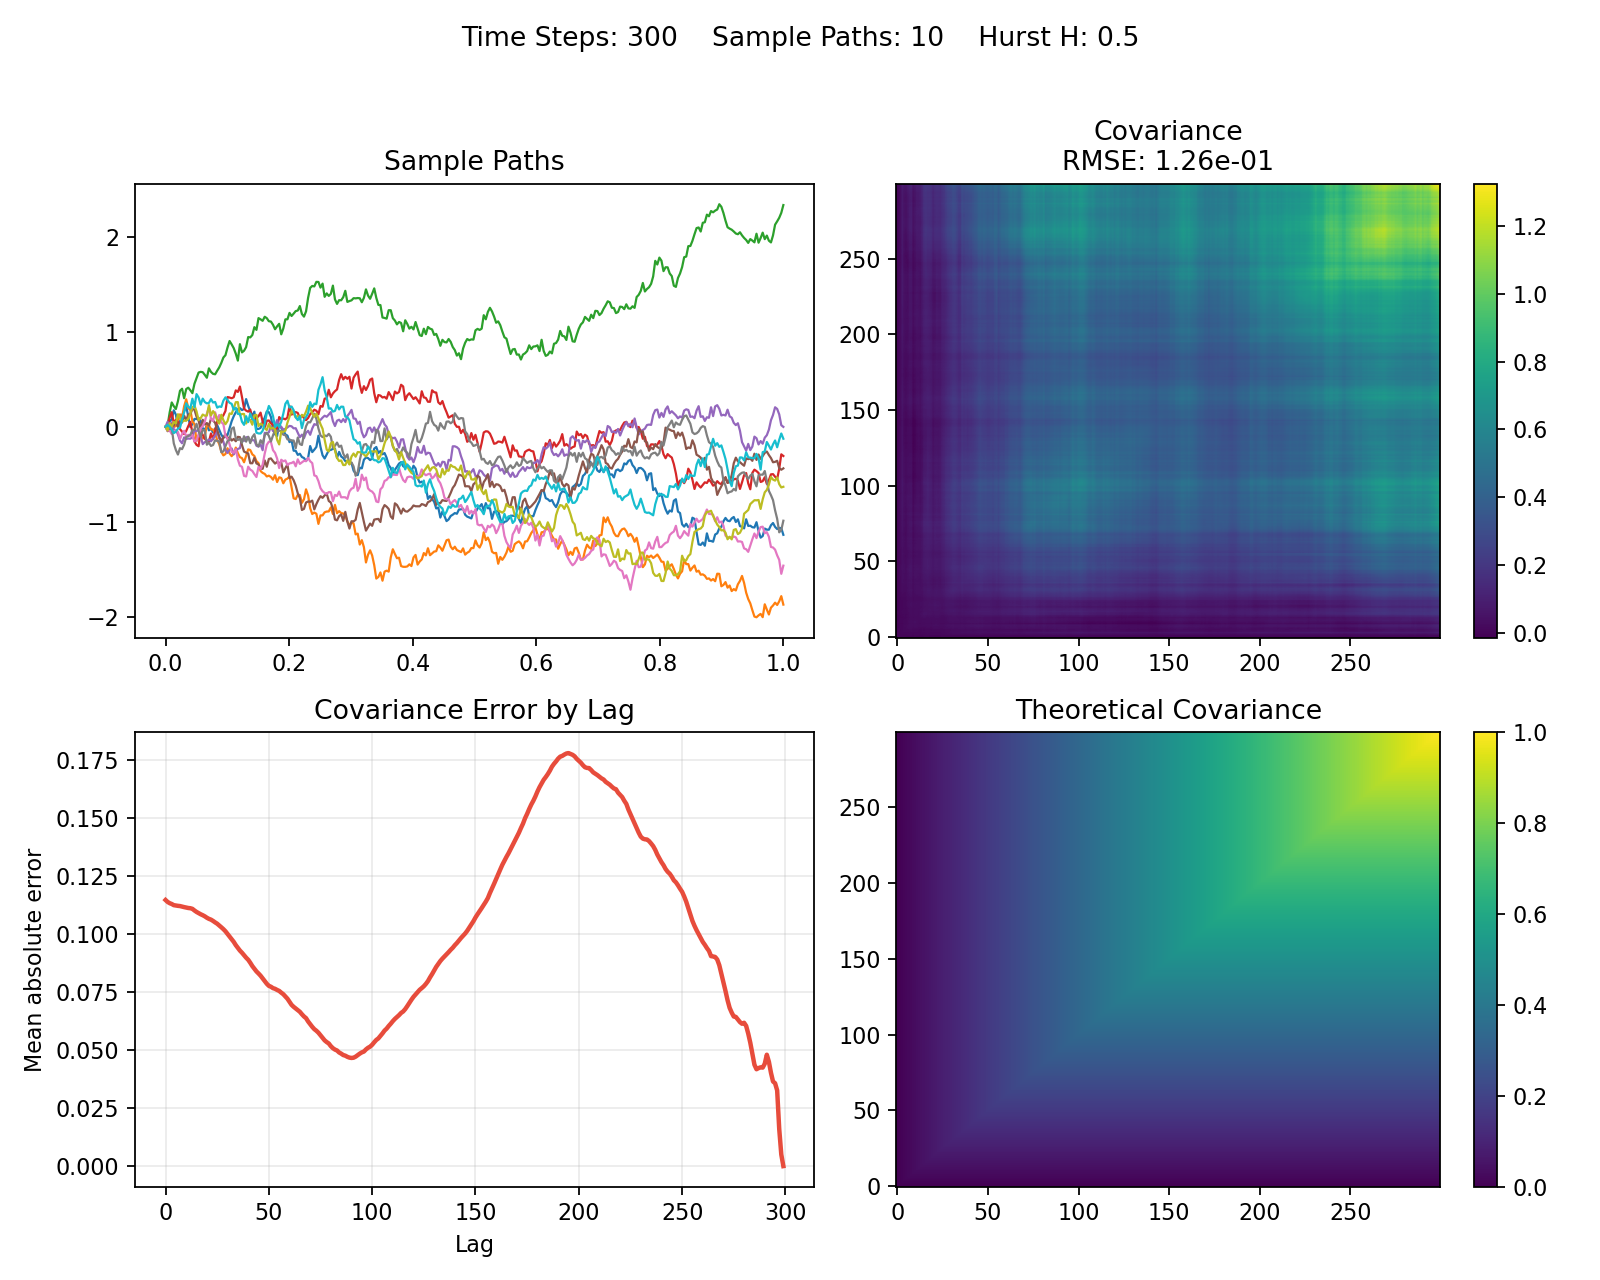
\includegraphics[width=\linewidth]{img/revisionato/2/fgm0.5.png}
\end{minipage}

\vspace{1.2cm}

%==================== ROW 2 ====================
\begin{minipage}[c][0.24\textheight][c]{0.50\textwidth}
\centering
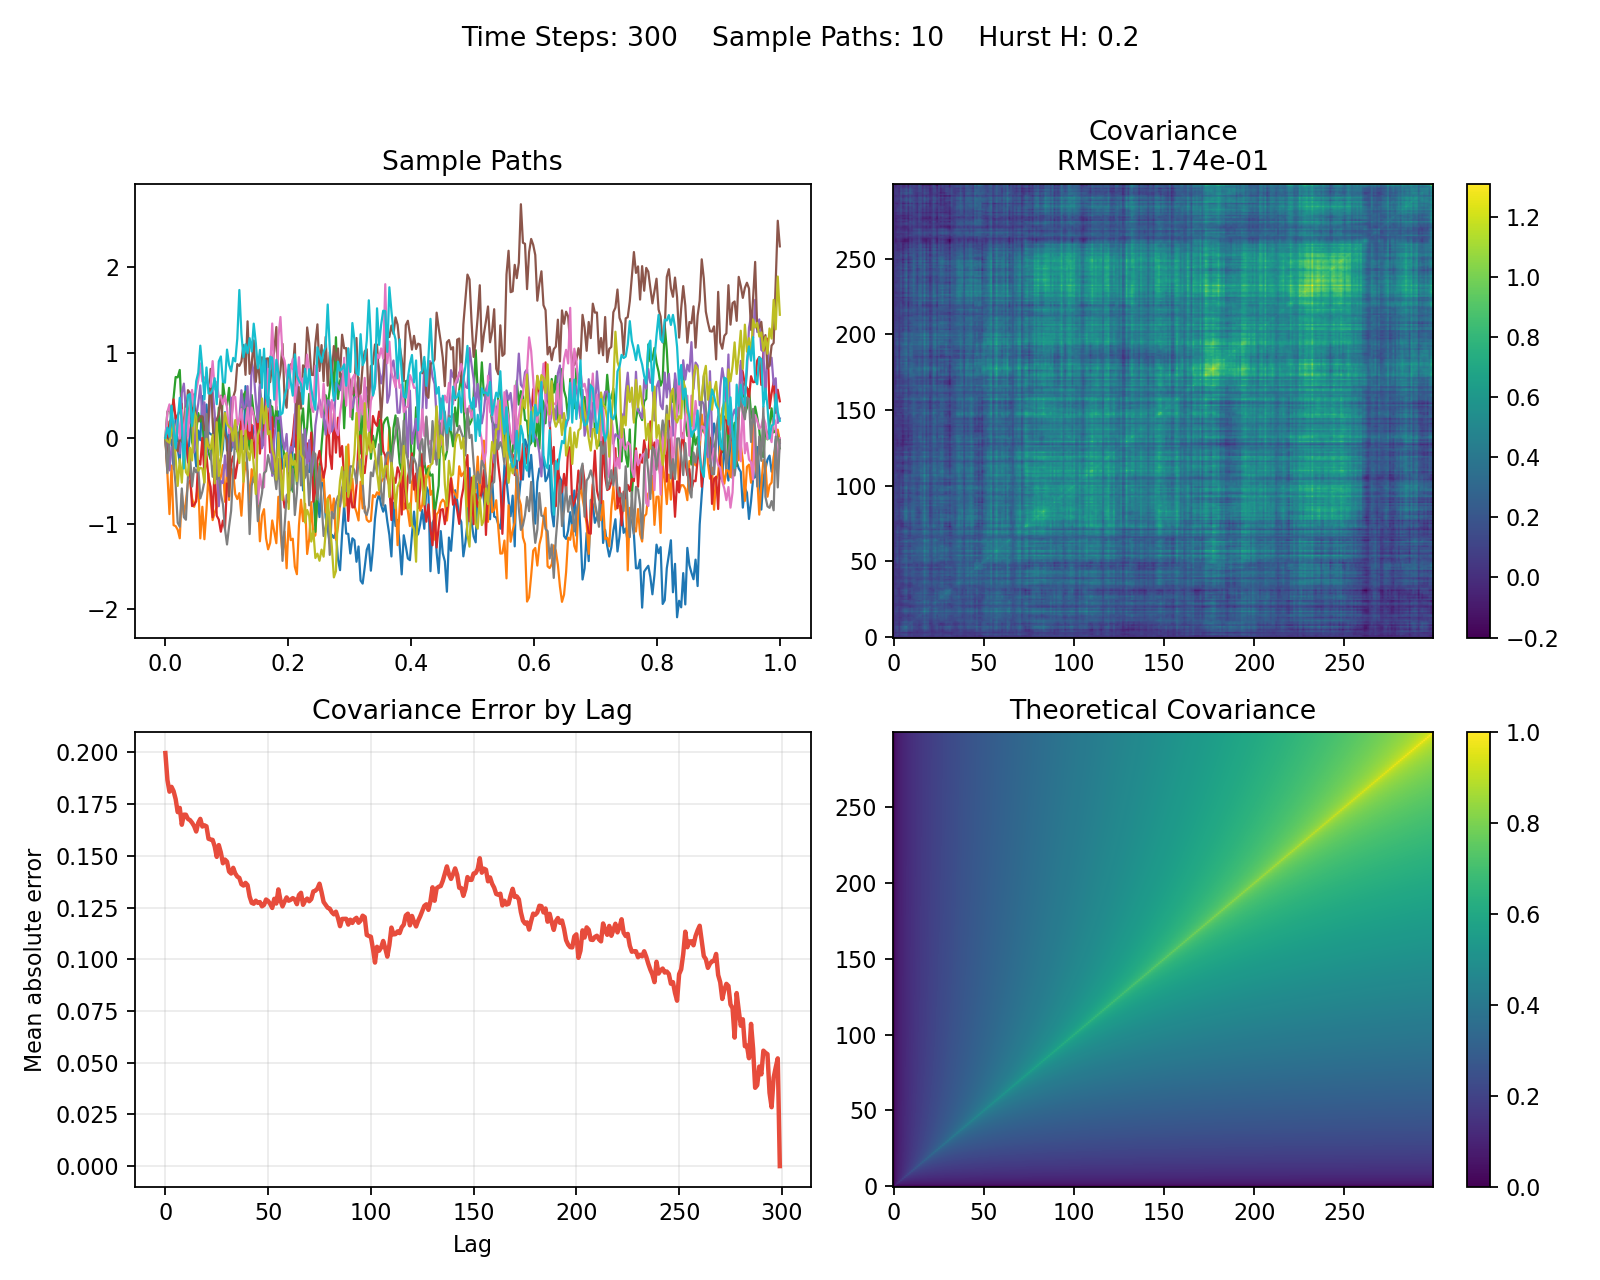
\includegraphics[width=\linewidth]{img/revisionato/2/fgm0.2.png}
\end{minipage}
\hfill
\begin{minipage}[c][0.24\textheight][c]{0.44\textwidth}
\normalsize
\textbf{Anti-persistent regime: \(H=0.2\).}

\vspace{0.3em}

When \(H<\tfrac12\), successive increments tend to have opposite signs. This negative correlation creates a stronger tendency toward local reversals, so the paths appear rougher and more irregular. Compared with the benchmark case \(H=0.5\), the motion oscillates more frequently and displays less local trend continuation. This regime is especially useful when one wants to emphasize roughness and short-term alternation in the trajectory.
\end{minipage}

\vspace{0.8cm}

%==================== ROW 3 ====================
\begin{minipage}[c][0.24\textheight][c]{0.44\textwidth}
\normalsize
\vspace{0.5cm}

\textbf{Persistent regime: \(H=0.8\).}

\vspace{0.3em}

When \(H>\tfrac12\), increments become positively correlated. As a consequence, upward moves are more likely to be followed by upward moves, and downward moves by downward moves. The resulting paths look smoother and more persistent than in the Brownian benchmark. Long local excursions become more visible, and the sample paths exhibit a stronger sense of directional continuity.
\end{minipage}
\hfill
\begin{minipage}[c][0.24\textheight][c]{0.50\textwidth}
\centering
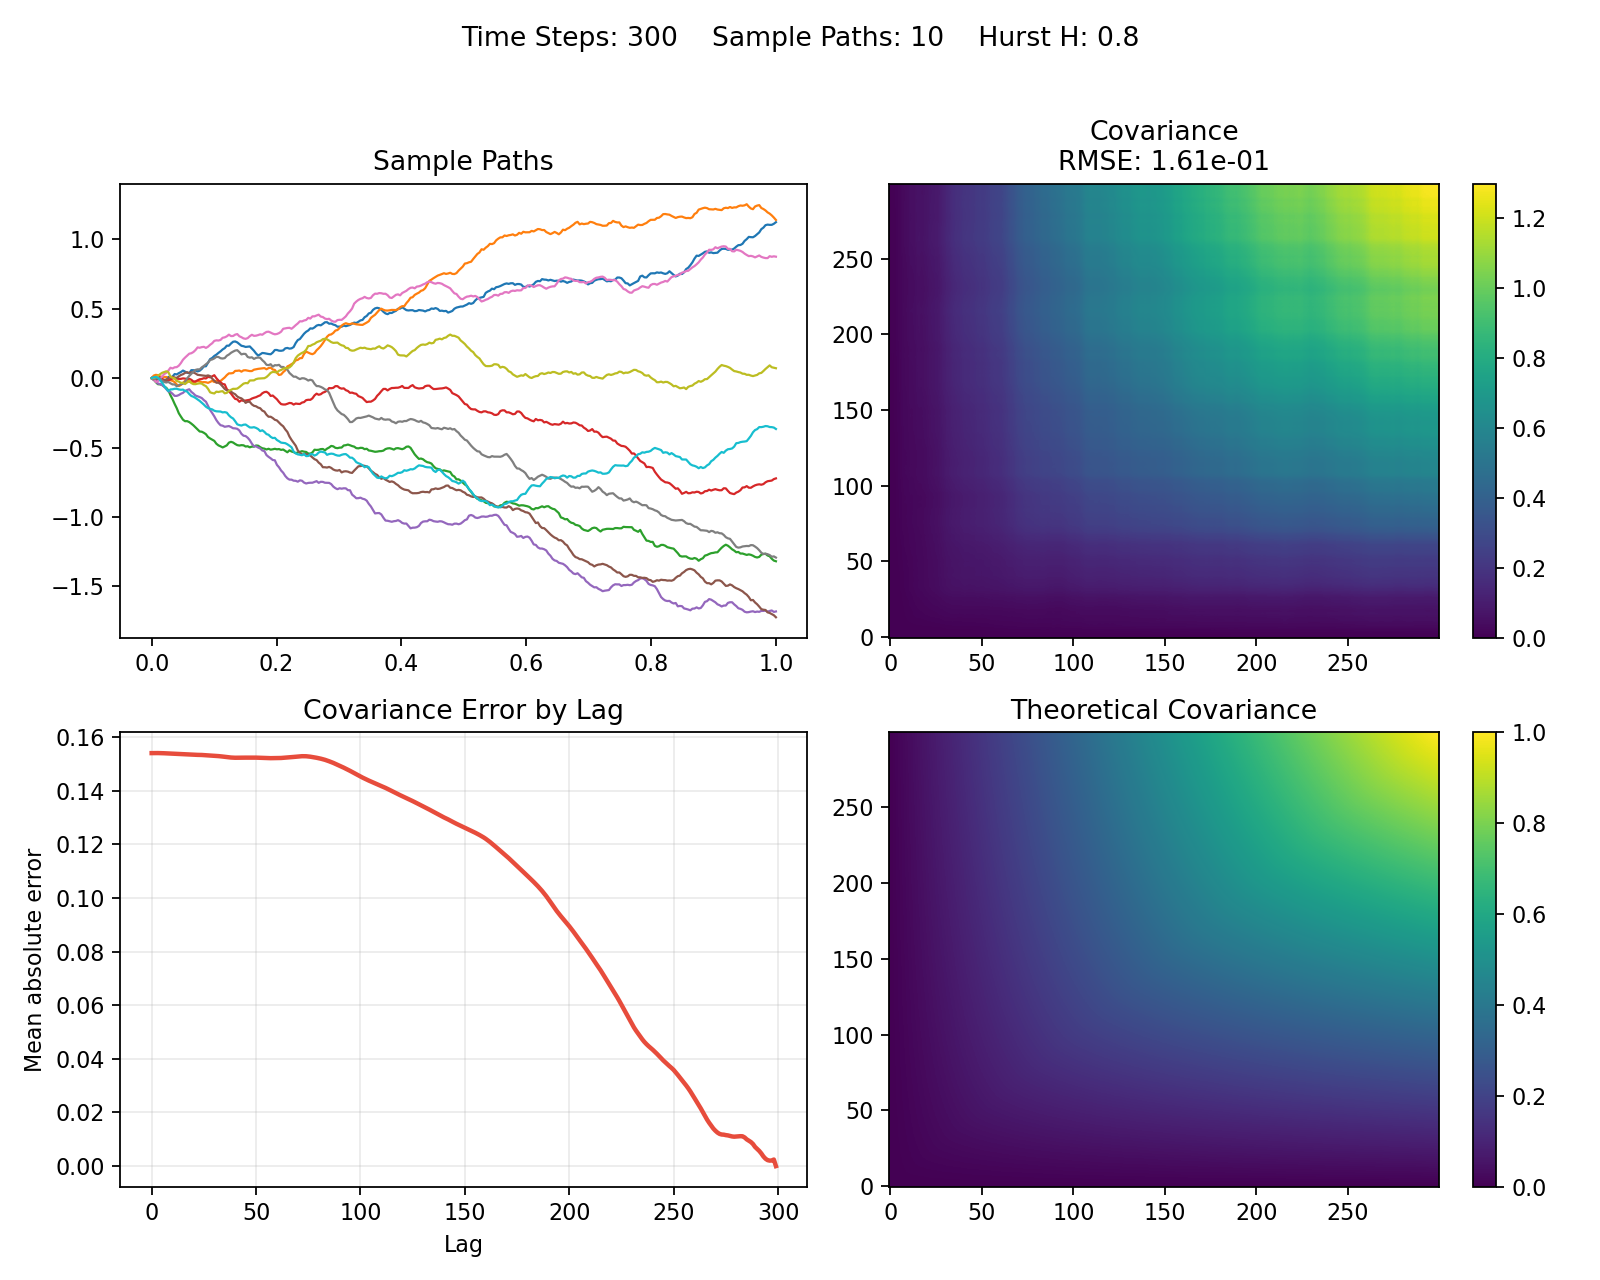
\includegraphics[width=\linewidth]{img/revisionato/2/fgm0.8.png}
\end{minipage}

\end{figure}

\vspace{0.5cm}

\section{Financial applications and computational challenges}

The interest in fractional Brownian motion within quantitative finance is mainly motivated by its ability to encode temporal dependence beyond the Markovian paradigm. In particular, when volatility is modeled as a latent process rather than as a directly traded asset, long-memory or roughness effects can become empirically relevant. This is one of the reasons why fractional-type models, and especially rough-volatility specifications, have attracted growing attention in the literature.

A natural interpretation of this point arises through the dynamics of log-volatility. If volatility exhibits dependence across multiple time scales, then a path-dependent Gaussian driver may provide a richer description than standard Brownian motion. In rough-volatility applications, this motivates the use of non-Markovian Gaussian structures to capture irregular short-term behavior together with persistent dependence.

This additional realism, however, comes at a cost. Once volatility is driven by a non-Markovian process, the model no longer admits the simple low-dimensional state representation available in classical diffusion frameworks. As a consequence, pricing and calibration become substantially more expensive. If one wishes to fit such a model to an implied-volatility surface, the procedure typically requires repeated simulation of the full volatility path, followed by repeated pricing across a grid of strikes and maturities.

The difficulty is not limited to pricing alone. Calibration requires solving an inverse problem: one must search over a parameter space until the model-generated prices or implied volatilities match the observed surface. In a non-Markovian setting, each candidate parameter vector may require a full path simulation, making the overall procedure too costly for live or large-scale applications.

This trade-off has motivated a parallel line of research based on surrogate methods. Instead of rerunning the full pricing model at each calibration step, one can attempt to learn the map from model parameters to implied-volatility surfaces through neural networks or other machine-learning approximators. If successful, such a surrogate can dramatically accelerate calibration. At the same time, the gain in speed comes with its own issues: approximation error, limited extrapolation power, and the fact that desirable structural properties, such as no-arbitrage consistency, are not automatically guaranteed.

For this reason, fractional Brownian motion should be viewed not as a free improvement over standard models, but as a richer modeling choice that trades analytical tractability for empirical flexibility. This trade-off makes simulation methodology especially important. We therefore begin with the Davies--Harte construction, which is a convenient way to generate fractional Gaussian noise and fractional Brownian motion with the correct covariance structure.

\section{Davies--Harte Simulation and Validation Code}

The trajectories displayed in the visual comparison above are most naturally generated from the increment process rather than from a direct covariance factorization. Among the available simulation methods, the Davies--Harte scheme is particularly convenient because it is both mathematically transparent and computationally efficient: it generates fractional Gaussian noise by embedding its covariance sequence into a circulant structure diagonalized by the FFT, and then recovers fractional Brownian motion by cumulative summation.

\paragraph{Inputs.} The basic inputs of the scheme are
\[
H\in(0,1), \qquad T>0, \qquad N\in\mathbb{N},
\]
where \(H\) is the Hurst parameter, \(T\) is the terminal time, and \(N\) is the number of time steps. We also define
\[
\Delta t = \frac{T}{N},
\qquad
t_n = n\Delta t,
\qquad n=0,1,\dots,N.
\]
As \(N\) increases, the grid becomes finer and the empirical statistics of the simulated process tend to align more closely with the theoretical ones.

\paragraph{Step 1: generate the time grid.} The first step is to discretize the interval \([0,T]\):
\[
t_n=n\Delta t,
\qquad n=0,1,\dots,N.
\]
This produces the \(N+1\) points on which the path will be represented.

\paragraph{Step 2: define the autocovariance of fractional Gaussian noise.} The Davies--Harte construction works directly with fractional Gaussian noise. Its autocovariance is
\[
\gamma_H(k)
=
\frac{1}{2}
\left(
|k+1|^{2H}
-
2|k|^{2H}
+
|k-1|^{2H}
\right),
\qquad k\in\mathbb{Z}.
\]
This formula determines the dependence structure of the increments and is the starting point of the whole algorithm.

\paragraph{Step 3: build the circulant covariance vector.} The key idea is to embed the covariance sequence into a circulant vector of length \(2N\). One convenient choice is
\[
c=
\bigl(
\gamma_H(0),\gamma_H(1),\dots,\gamma_H(N-1),0,
\gamma_H(N-1),\dots,\gamma_H(1)
\bigr).
\]
This step is crucial because circulant matrices are diagonalized by the discrete Fourier transform, which makes the method computationally efficient.

\paragraph{Step 4: compute the embedded eigenvalues via FFT.} Let
\[
m=2N.
\]
Applying the FFT to the circulant vector produces the embedded eigenvalues
\[
\lambda_j=\Re\bigl(\mathrm{FFT}(c)_j\bigr),
\qquad j=0,\dots,m-1.
\]
Since this is a covariance embedding, the relevant eigenvalues must be nonnegative up to numerical tolerance. In practice, one checks this explicitly before proceeding.

\paragraph{Step 5: generate the complex Gaussian vector.} The next step is to construct a complex Gaussian vector \(Z=(Z_0,\dots,Z_{m-1})\) with the conjugate symmetry required by the inverse transform. Let \(\xi_k,\eta_k\) be independent standard normal random variables. Then define
\[
Z_0=\sqrt{\lambda_0}\,\xi_0,
\qquad
Z_N=\sqrt{\lambda_N}\,\xi_N,
\]
and for \(k=1,\dots,N-1\),
\[
Z_k
=
\sqrt{\frac{\lambda_k}{2}}
\left(\xi_k+i\eta_k\right),
\qquad
Z_{m-k}=\overline{Z_k}.
\]
This is the most delicate part of the scheme. The conjugate assignment ensures that the inverse FFT will return a real-valued Gaussian sequence.

\paragraph{Step 6: apply the inverse FFT and restore the time scale.} Applying the inverse FFT to \(Z\) produces a realization of fractional Gaussian noise. However, one must be careful with scaling. In NumPy, the inverse FFT includes a factor \(1/m\), so a correction is needed. In addition, the correct time scale must be restored through \(\Delta t^H\). The simulated increments are therefore
\[
\Delta B_j^H
=
\Delta t^H\,\sqrt{m}\,
\Re\!\left(\mathrm{IFFT}(Z)_j\right),
\qquad j=0,\dots,N-1.
\]
The factor \(\sqrt{m}\) corrects the normalization introduced by the inverse FFT, while \(\Delta t^H\) ensures that
\[
\Var(\Delta B_j^H)=\Delta t^{2H}.
\]

\paragraph{Step 7: recover fractional Brownian motion by cumulative summation.} Once the increments have been generated, fractional Brownian motion is obtained by accumulation:
\[
B_0^H=0,
\qquad
B_{t_n}^H=\sum_{j=0}^{n-1}\Delta B_j^H,
\qquad n=1,\dots,N.
\]
This final step is conceptually simple but essential: the whole simulation procedure reduces to generating the correct correlated Gaussian increments and summing them.

\section{Simulation and confirmation against theoretical results}

Once the simulation scheme has been implemented, the next question is whether the output is actually correct. A plausible-looking path is not enough: even a small scaling mistake inside the FFT or inverse FFT can generate visually convincing trajectories whose empirical moments do not match the theoretical ones. For this reason, the simulation should be validated against the variance of fractional Gaussian noise, the variance of fractional Brownian motion, and the full covariance kernel of the process.

\paragraph{Variance of the increments and of the process.} The most immediate diagnostic consists in comparing empirical and theoretical variances. For the simulated fractional Gaussian noise, the theoretical variance is
\[
\Var(\Delta B_j^H)=\Delta t^{2H}.
\]
For fractional Brownian motion itself, the variance at time \(t_n\) is
\[
\Var(B_{t_n}^H)=t_n^{2H}.
\]
These two identities provide a simple but informative consistency check. The first confirms that the increment process has been scaled correctly, while the second confirms that the cumulative summation from fractional Gaussian noise to fractional Brownian motion has been implemented properly.

In practice, one generates many paths, computes empirical variances, and compares them to the theoretical targets. As the number of simulated paths and the grid resolution increase, the discrepancy should decrease.

\paragraph{Covariance-matrix confirmation.} A more informative validation compares the full empirical covariance matrix of the simulated process to the theoretical covariance kernel
\[
\Gamma_{ij}
=
\Cov(B_{t_i}^H,B_{t_j}^H)
=
\frac12\left(
t_i^{2H}+t_j^{2H}-|t_i-t_j|^{2H}
\right).
\]
Given \(M\) simulated paths \(B^{(1)},\dots,B^{(M)}\), one can estimate the empirical covariance matrix by
\[
\widehat{\Gamma}_{ij}
=
\frac{1}{M-1}
\sum_{r=1}^{M}
\left(B_{t_i}^{(r)}-\overline{B}_{t_i}\right)
\left(B_{t_j}^{(r)}-\overline{B}_{t_j}\right),
\]
where \(\overline{B}_{t_i}\) is the empirical mean at time \(t_i\). The discrepancy between empirical and theoretical covariance can then be summarized by the root mean squared error
\[
\mathrm{RMSE}
=
\left(
\frac{1}{(N+1)^2}
\sum_{i=0}^{N}\sum_{j=0}^{N}
\bigl(\widehat{\Gamma}_{ij}-\Gamma_{ij}\bigr)^2
\right)^{1/2}.
\]

This is the natural theoretical benchmark for the simulated paths shown earlier. The visual comparison in the previous figure illustrates how the geometry of the trajectories changes with \(H\); the covariance validation presented here explains why those paths are statistically consistent with the definition of the process.

\paragraph{Error decay in \(N\) and \(M\).} A correct implementation should not only reproduce the covariance structure at one fixed parameter choice, but should also exhibit the expected improvement as the numerical inputs increase. There are two natural directions along which to check this.

First, increasing \(N\) refines the time grid and improves the empirical representation of the increment process. In particular, one may study how the RMSE associated with the variance of fractional Gaussian noise decreases as the grid becomes finer.

Second, increasing the number of simulated paths \(M\) improves the empirical estimation of the covariance matrix. Since covariance estimation is a Monte Carlo object, the RMSE should decay at the standard rate
\[
\mathrm{RMSE}=O(M^{-1/2}).
\]
This provides a useful benchmark: if the implementation is correct, increasing the sample size should reduce the covariance estimation error approximately at that rate.


\begin{algorithm}[H]
\caption{Validation diagnostics before the convergence figure}
\DontPrintSemicolon
\For{each grid size \(N\)}{
  simulate fractional Gaussian noise and compare empirical increment variance with \(\Delta t^{2H}\)\;
}
\For{each number of paths \(M\)}{
  estimate the empirical covariance matrix of \(B^H\)\;
  compare it with the theoretical covariance kernel and record the RMSE\;
}
plot both error curves against their theoretical decay benchmarks\;
\end{algorithm}

\begin{figure}[H]
\centering
\begin{minipage}[t]{0.48\textwidth}
\centering
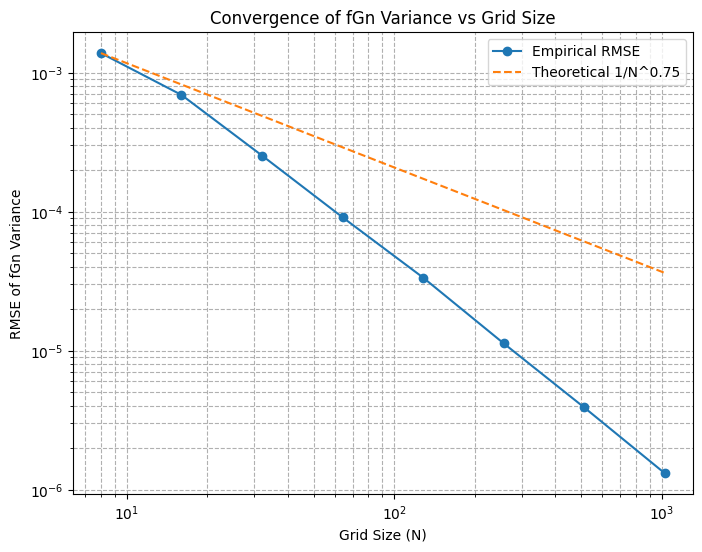
\includegraphics[width=\linewidth]{img/2/img_4.png}
\end{minipage}
\hfill
\begin{minipage}[t]{0.48\textwidth}
\centering
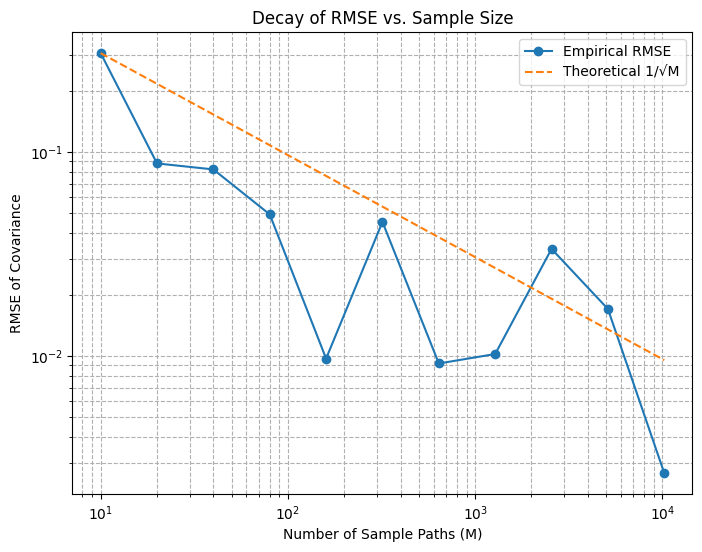
\includegraphics[width=\linewidth]{img/2/img_5.png}
\end{minipage}
\caption{Convergence diagnostics for the Davies--Harte implementation. The left panel compares the empirical decay of the RMSE for the variance of fractional Gaussian noise with the theoretical benchmark as the grid size \(N\) increases. The right panel compares the empirical decay of the covariance RMSE with the Monte Carlo reference rate \(1/\sqrt{M}\) as the number of simulated paths \(M\) grows.}
\label{fig:fbm_convergence_diagnostics}
\end{figure}

Taken together, these checks provide a coherent validation strategy. First, one verifies that the increment process and the accumulated process have the correct variance scaling. Then, one compares the full empirical covariance matrix to the theoretical covariance kernel. Finally, one checks that the numerical error decreases in the expected way as \(N\) and \(M\) increase. Figure \ref{fig:fbm_convergence_diagnostics} illustrates these convergence patterns directly. The decay in the left panel is consistent with improved variance accuracy on finer grids, while the right panel shows the expected overall reduction in covariance error as the sample size increases, despite the visible finite-sample noise typical of Monte Carlo experiments.

\section{Problems of Davies--Harte simulations}

The Davies--Harte scheme is an elegant and efficient way to generate fractional Gaussian noise and, by cumulative summation, fractional Brownian motion. For offline Monte Carlo experiments it is extremely useful, since it reproduces the target covariance structure accurately and does so at relatively low computational cost. For the purposes of the present paper, however, this efficiency comes with an important limitation: the construction is fundamentally global rather than causal.

The issue is not that fractional Brownian motion itself depends on future information. It does not. The issue is instead numerical and structural. In the Davies--Harte scheme, one fixes the entire time grid in advance, embeds the covariance sequence into a circulant structure, applies spectral methods, and generates the full trajectory at once. In this sense, the algorithm requires \emph{global path knowledge}: the desired covariance structure is enforced through a construction that acts on the whole path simultaneously, rather than through a recursive state update based only on past shocks.

This point matters in sequential financial applications. In market making, filtering, and related control problems, one typically wants a representation that evolves forward in time as new information arrives. At each time \(t\), the state should be updated causally from what is already known, without relying on a simulation architecture that is tied to the full terminal horizon. From this perspective, Davies--Harte is mathematically valid and computationally efficient, but it is not the most natural language for an online control problem.

A related limitation appears in model fitting. If one were to use a non-Markovian volatility specification driven by fractional Brownian motion and calibrate it to an implied-volatility surface, then in the absence of a closed-form pricing formula one would typically need repeated Monte Carlo simulation. For each parameter choice, one must simulate the full volatility path, generate prices over a grid of strikes and maturities, compare the model output with the observed surface, and then iterate over the parameter space. Even if the underlying simulator is efficient, this overall calibration loop quickly becomes computationally intensive and may become impractical in a live setting.

There is therefore a genuine trade-off. On the one hand, rough or long-memory dynamics may capture empirically relevant dependence structures more faithfully than classical Markovian diffusions. On the other hand, these gains do not come for free: they are purchased with greater numerical cost and with the loss of a simple recursive state representation. In particular, while Davies--Harte is well suited for global path generation and covariance-based validation, it is not the most convenient framework when the final objective is a causal simulation architecture for sequential pricing or inventory control.

For these reasons, the Davies--Harte scheme should be regarded as an excellent benchmark for simulation and validation, but not yet as the most natural representation for control-oriented modeling. What is needed next is a formulation that preserves memory while making causality explicit. This is precisely the role of Gaussian Volterra processes: they replace the global covariance viewpoint with a kernel-based construction in which the state at time \(t\) depends on past noise only. This makes them a more natural starting point for rough-volatility simulation, approximation, and eventually market-making control.

%%%%%%%%%%%%%%%%%%%%%%%%%%%%%%%%%%%%%%%%%%%%%%%%
%%%%%%%%%%%%%%%%%%%%%%%%%%%%%%%%%%%%%%%%%%%%%%%%
%%%%%%%%%%%%%%%%%%%%%%%%%%%%%%%%%%%%%%%%%%%%%%%%

\chapter{Volterra Gaussian Processes and Causality}
\miniabstract{The previous chapter introduced fractional Brownian motion through its covariance structure and the global Davies--Harte simulator. This chapter replaces that covariance-first view with a causal Volterra integral, where past information enters explicitly through a kernel and the state can be updated as new shocks arrive.}

\paragraph{From global covariance to causal kernels.}

Given a Brownian driver, the Volterra kernel assigns a weight to every shock that is already observable at time \(t\). This separates two roles that a covariance-first simulator leaves implicit: the support condition determines which shocks may enter the state, while the kernel profile determines their relative influence. That distinction is useful in a pricing engine or control loop because it exposes the information set used by each update.

This is the main difference with covariance-based simulation methods such as Davies--Harte. There, the objective is to sample the entire path with the correct law, and this is done through a global embedding of the covariance sequence. In a Volterra representation, by contrast, one builds the process forward in time through a weighted accumulation of Brownian shocks. The weights are determined by the kernel, and therefore the kernel becomes the object that controls both the dependence structure and the geometry of the paths.

\section{General Volterra representation}

\begin{definition}[Gaussian Volterra process]
Let \(W\) be a standard Brownian motion and let \(K(t,s)\) be a measurable kernel such that
\(
K(t,s)=0 \; \text{for } s>t,
\; \text{and}  \;
\int_0^t K(t,s)^2\,ds<\infty
\; \text{for all } t\ge 0.
\)
A \emph{Gaussian Volterra process} is a process of the form
\[
X_t=\int_0^t K(t,s)\,dW_s.
\]
\end{definition}

The condition \(K(t,s)=0\) for \(s>t\) is the mathematical expression of causality: the process at time \(t\) depends only on shocks observed before time \(t\). The entire covariance structure is therefore encoded in the kernel itself.

\section{Covariance induced by the kernel}

The key step is to show how the kernel determines the covariance of the process. Since the stochastic integral is centered, one expects the covariance to reduce to an expectation of a product of integrals, which can then be simplified by It\^o isometry.

\begin{proposition}[Covariance induced by a Volterra kernel]
Let
\[
X_t=\int_0^t K(t,s)\,dW_s.
\]
Then for any \(s,t\ge 0\),
\[
\Cov(X_s,X_t)
=
\int_0^{s\wedge t} K(s,u)K(t,u)\,du.
\]
\end{proposition}

\begin{proof}
Since \(X_s\) and \(X_t\) are centered Gaussian variables,
\[
\Cov(X_s,X_t)=\E[X_sX_t].
\]
Using the stochastic integral representation,
\[
\E[X_sX_t]
=
\E\!\left[
\left(\int_0^s K(s,u)\,dW_u\right)
\left(\int_0^t K(t,v)\,dW_v\right)
\right].
\]
By It\^o isometry for products of stochastic integrals,
\[
\E\!\left[
\left(\int_0^s f(u)\,dW_u\right)
\left(\int_0^t g(v)\,dW_v\right)
\right]
=
\int_0^{s\wedge t} f(u)g(u)\,du.
\]
Applying this with \(f(u)=K(s,u)\) and \(g(u)=K(t,u)\) gives
\[
\Cov(X_s,X_t)
=
\int_0^{s\wedge t} K(s,u)K(t,u)\,du. \qedhere
\]
\end{proof}
    
This identity is the central bridge between the process and its second-order structure. It shows that once the kernel is selected, the covariance is no longer imposed externally: it is generated mechanically by the causal accumulation of Brownian shocks.

\paragraph{Why causality matters.}

The formula above also explains why the upper integration limit becomes \(s\wedge t\). If \(u>s\), then \(K(s,u)=0\) by causality; similarly, if \(u>t\), then \(K(t,u)=0\). Hence the product \(K(s,u)K(t,u)\) can only be nonzero when \(u\le s\) and \(u\le t\), which is equivalent to \(u\le s\wedge t\).

This point is important in sequential financial applications. In an online control problem one does not want a representation that is tied to the whole terminal horizon or to a global covariance embedding. Instead, one wants a state variable that can be updated as new information arrives. A Volterra process has exactly this interpretation: it is built from past noise only, with the memory of the process encoded through the kernel.

At the same time, causality should not be confused with Markovianity. A causal Volterra process may still be strongly non-Markovian. The value at time \(t\) does not depend on future noise, but it may depend on the entire past history of the driving Brownian motion. This is precisely what makes Volterra processes flexible enough to reproduce both rough and persistent behavior.

\section{Discretization and non-Markovian structure}

Once the Volterra representation is available, discretization is conceptually simple. Fix a horizon \(T>0\) and choose a uniform grid
\(
0=t_0<t_1<\cdots<t_n=T,
\quad
t_i=\frac{iT}{n},
\quad
\Delta t=\frac{T}{n}.
\)
Let
\[
\Delta W_j = W_{t_{j+1}}-W_{t_j},
\quad
\Delta W_j\sim \mathcal{N}(0,\Delta t),
\]
with independent increments across \(j\). A Riemann--It\^o approximation of the stochastic integral then yields
\[
X_{t_i}
\approx
\sum_{j=0}^{i-1} K(t_i,t_j)\,\Delta W_j.
\]

This discrete expression is the natural simulation recipe: choose a kernel, generate Brownian increments, and at each time point accumulate the past shocks with the appropriate weights. After the grid values have been obtained, one may visualize the path through piecewise linear interpolation, which is simply the numerical analogue of joining the dots.

\paragraph{Iterative construction.}

The discretized Volterra process can be built step by step from left to right. At the first nonzero grid point,
\[
X_{t_1}\approx K(t_1,t_0)\,\Delta W_0.
\]
At the next step,
\[
X_{t_2}\approx K(t_2,t_0)\,\Delta W_0 + K(t_2,t_1)\,\Delta W_1,
\]
and more generally
\[
X_{t_i}\approx \sum_{j=0}^{i-1} K(t_i,t_j)\,\Delta W_j.
\]

This already makes the causal structure visible: to build \(X_{t_i}\), one needs only the Brownian increments observed before time \(t_i\). But the same formula also shows why the process is non-Markovian in general. Indeed, the increment from \(t_{i-1}\) to \(t_i\) is
\[
X_{t_i}-X_{t_{i-1}}
\approx
K(t_i,t_{i-1})\,\Delta W_{i-1}
+
\sum_{j=0}^{i-2}
\bigl(K(t_i,t_j)-K(t_{i-1},t_j)\bigr)\,\Delta W_j.
\]
Unless the kernel is trivial, the new increment depends not only on the most recent shock, but also on the entire path history through all previous \(\Delta W_j\). This is exactly the discrete manifestation of non-Markovianity.

The special case in which this dependence disappears is standard Brownian motion. If one chooses the trivial kernel
\(
K(t,s)=1,
\; 0\le s<t,
\)
then
\[
X_t=\int_0^t dW_s = W_t,
\]
and the increment structure collapses to the familiar Markovian setting. This observation is useful: the Volterra framework contains Brownian motion as a limiting benchmark, but becomes genuinely non-Markovian as soon as the kernel introduces memory.
\section{Representative kernels and induced dynamics}

The flexibility of the Volterra representation comes from the choice of kernel. Different kernels induce different covariance structures and therefore different path dynamics.

\textbf{Brownian kernel}

The simplest example is
\(
K_{\mathrm{BM}}(t,s)=1.
\)
This reproduces standard Brownian motion,
\[
X_t=\int_0^t dW_s=W_t.
\]
In this case the Volterra construction is mathematically correct but computationally unnecessary, since Brownian motion can be simulated directly from independent Gaussian increments. Its main value here is conceptual: it shows that a Markovian process is contained as a special case in the broader Volterra family.

\textbf{Exponential kernel and mean reversion}

A second important example is the exponential kernel
\[
K_{\theta}(t,s)=e^{-\theta(t-s)}\mathbf{1}_{\{0\le s<t\}},
\qquad \theta>0.
\]
This kernel generates the Ornstein--Uhlenbeck process
\[
X_t=\int_0^t e^{-\theta(t-s)}\,dW_s,
\]
which solves the mean-reverting stochastic differential equation
\[
dX_t=-\theta X_t\,dt + dW_t.
\]
The exponential decay gives more weight to recent shocks than to distant ones, producing the familiar pull back toward the mean.

\textbf{Fractional-type kernel and roughness}

The rough-volatility literature is driven by singular power-law kernels. A simple causal prototype is
\[
\widetilde{K}_H(t,s)
=
\sqrt{c_H}\,(t-s)^{H-\frac12}\mathbf{1}_{\{0\le s<t\}},
\qquad
c_H=\frac{\Gamma(2H+1)}{2\,\Gamma(H+\frac12)^2},
\]
with \(H\in(0,1)\). The kernel is singular near the diagonal \(t=s\), which means that very recent history receives a particularly large weight. This is what generates roughness when \(H<\tfrac12\) and smoother, more persistent behavior when \(H>\tfrac12\). In the diagnostic implementation, the boundary value \(H=\tfrac12\) is treated separately with the exact Brownian kernel \(K(t,s)=\mathbf{1}_{\{s<t\}}\), so the resulting process is standard Brownian motion rather than the limiting normalization of this prototype.

\begin{remark}[Exact versus simplified fractional kernels]
Standard fractional Brownian motion admits an exact Volterra representation with a kernel \(K_H(t,s)\), but the closed form is more involved than a simple power law. In numerical intuition and in many rough-volatility approximations, one instead works with a tractable causal power-law kernel whose local behavior reproduces the desired roughness exponent. This chapter follows that practical route, since the goal is to prepare a simulation architecture rather than a complete classification of exact Gaussian representations.
\end{remark}

\section{Visual comparison across Hurst parameters}

The effect of the kernel is easiest to understand visually. In the panels below, the left block for each value of \(H\) illustrates the iterative construction of the process through a filtration window: as the window expands, the path is built using progressively more past information, exactly as required by causality. The right block shows the corresponding Volterra diagnostics, including sample paths, the kernel heat map, the Brownian driver, the full support of representative kernel slices, and the covariance induced by the discrete kernel. The reported RMSE compares that induced covariance with the standard fractional-Brownian target; it is zero up to numerical precision in the Brownian benchmark and need not vanish for the simplified power-law kernels.

\begin{algorithm}[H]
\caption{Reading the Volterra construction panels}
\DontPrintSemicolon
choose a causal kernel \(K_H(t,s)\) and Brownian increments \(\Delta W_j\)\;
\For{each time index \(i\)}{
  compute \(X_{t_i}\approx\sum_{j<i}K_H(t_i,t_j)\Delta W_j\) using past shocks only\;
  reveal the filtration window that is available at that step\;
}
plot the iterative path construction beside the kernel, noise, causality, and covariance diagnostics\;
\end{algorithm}



\begin{figure}[H]
\vspace{0cm}
\centering
\begin{minipage}[t]{0.44\textwidth}
\vspace{0cm}
\normalsize


\textbf{Benchmark regime: \(H=0.5\).}

The value \(H=\tfrac12\) is the exact Brownian benchmark. Here \(K(t,s)=1\) for \(s<t\) and \(K(t,s)=0\) for \(s\ge t\), so each kernel slice is flat over the observed past and drops to zero over the future. Consequently \(X_t=\int_0^t dW_s=W_t\): disjoint increments are independent and there is no fractional memory, although the construction remains causal because no future shock enters the state. The kernel heat map and the covariance heat map use the same numerical color range \([0,1]\), but their shapes differ by construction: the first is the binary support kernel, while the second is \(\Cov(W_t,W_s)=\min(t,s)\).

\vspace{0.5cm}
\centering
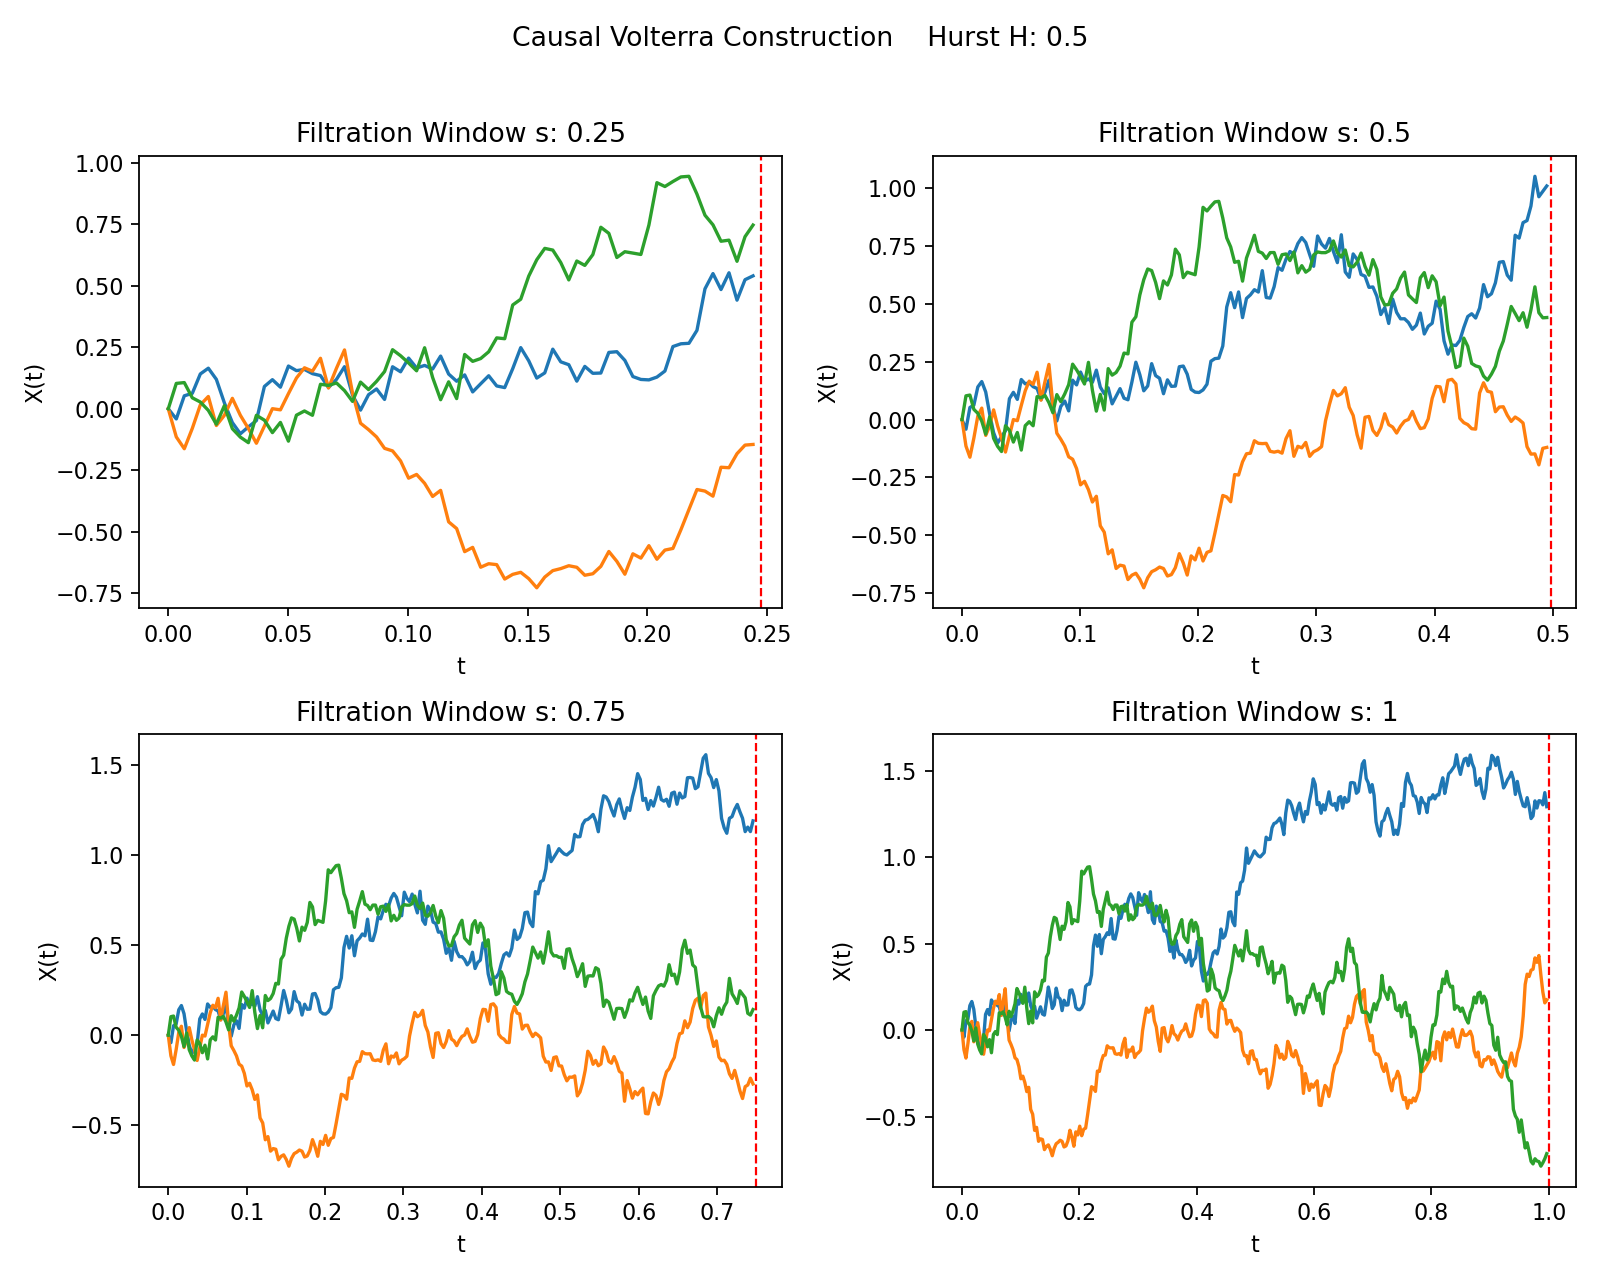
\includegraphics[width=\linewidth]{img/revisionato/2/iterative0.5.png}
\end{minipage}
\hfill
\begin{minipage}[t]{0.54\textwidth}
\vspace{0.2cm}
\centering
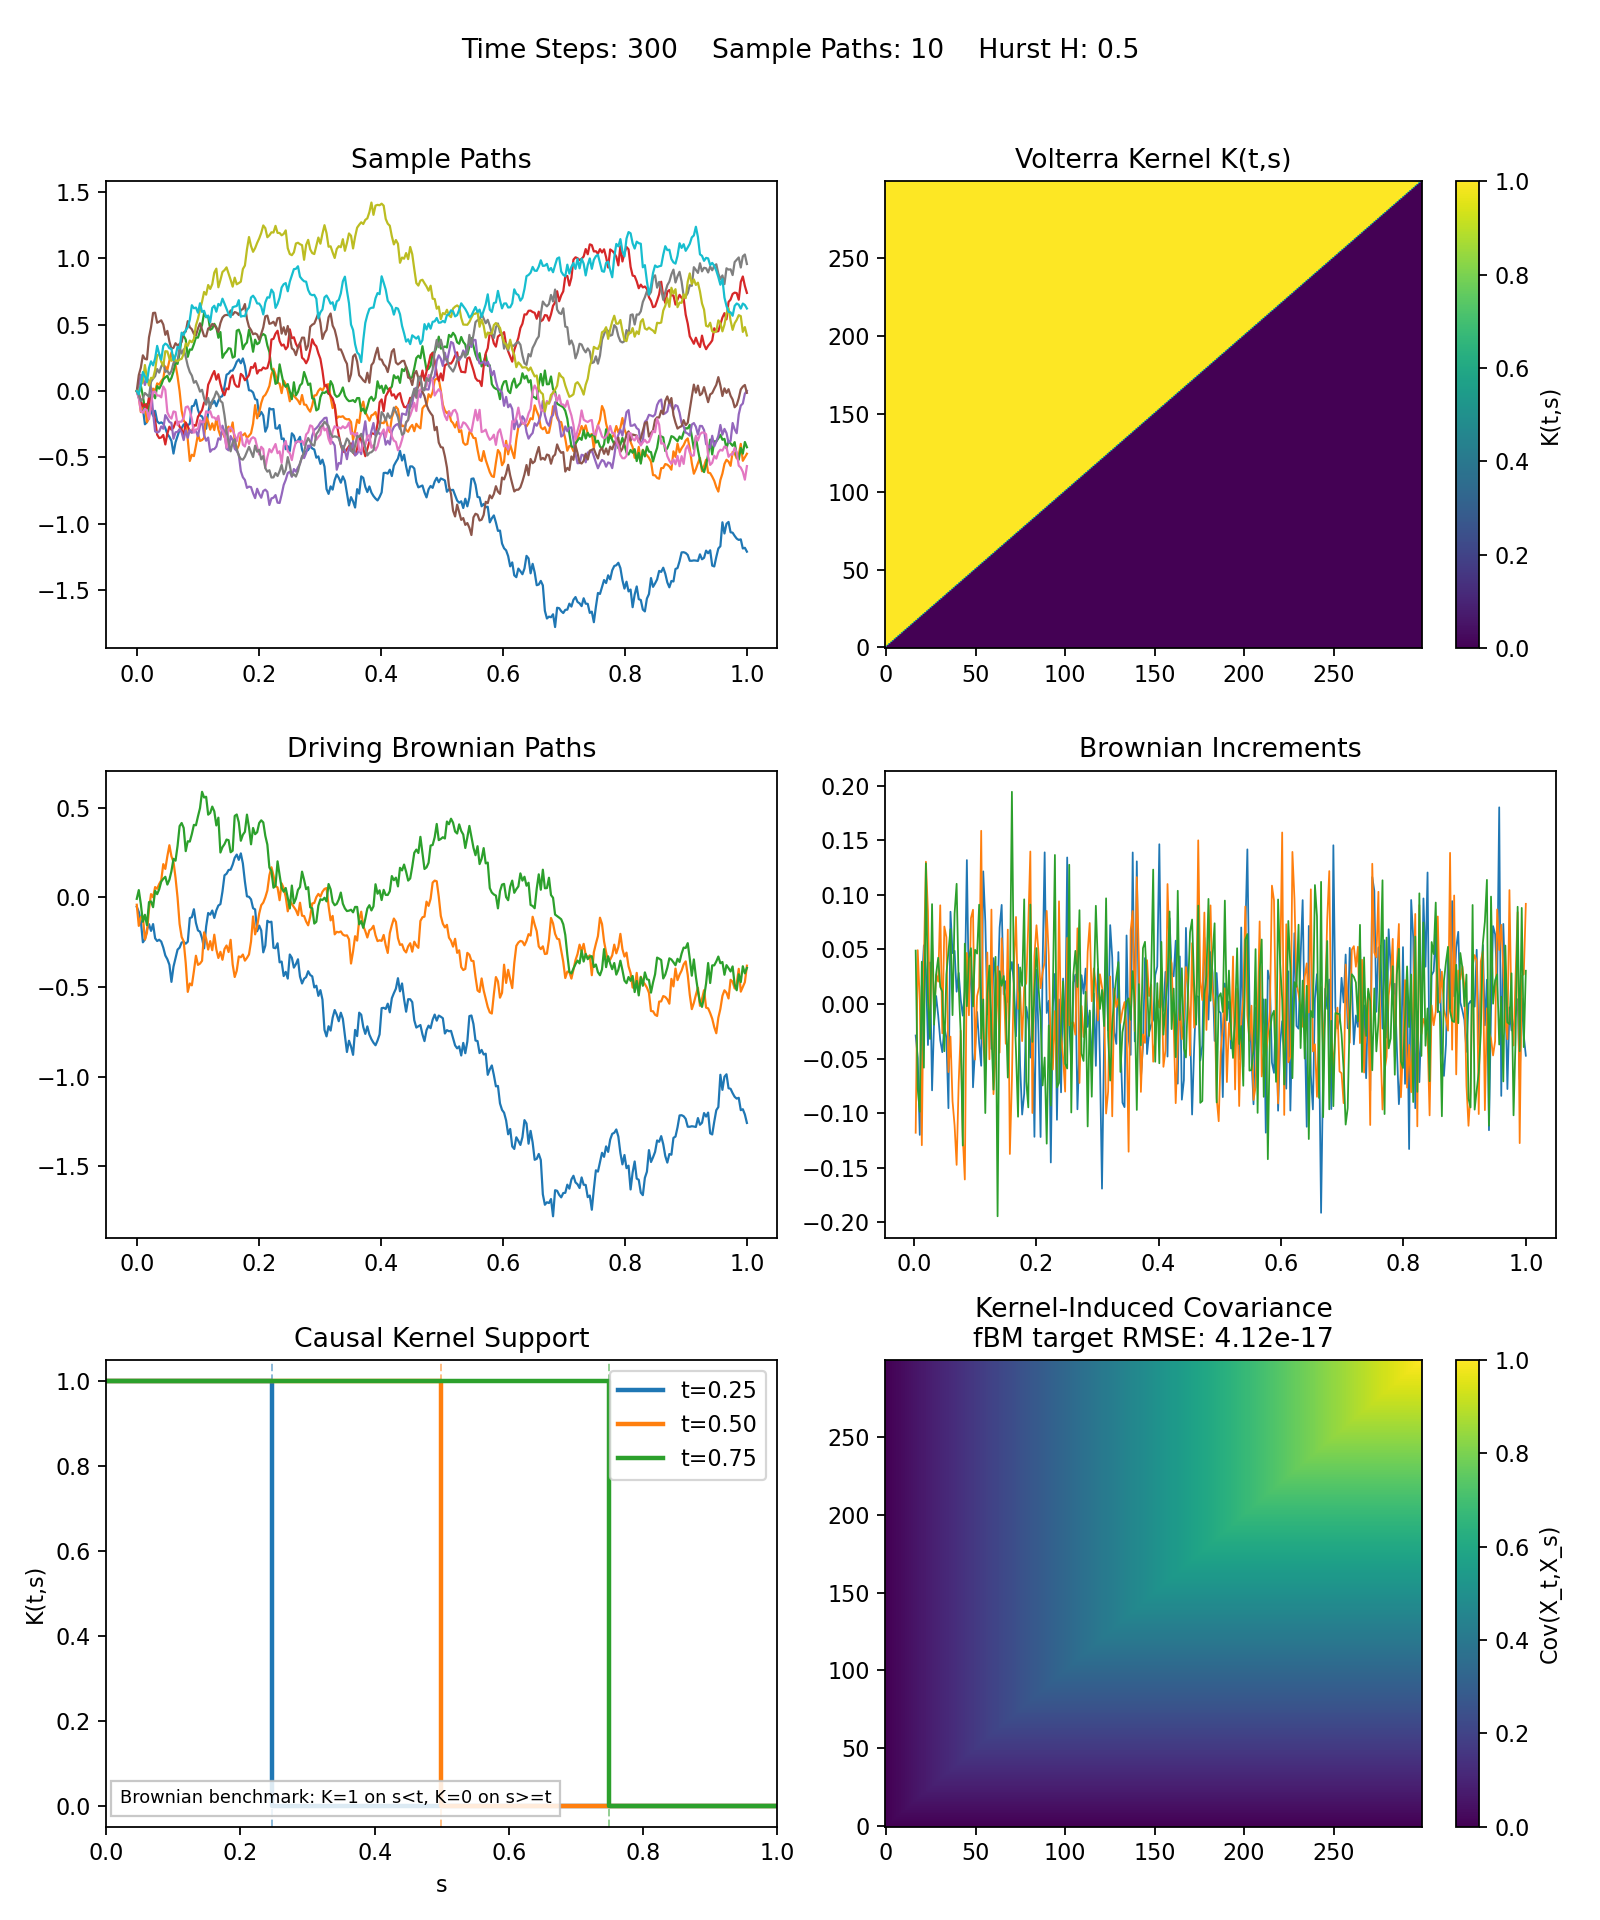
\includegraphics[width=\linewidth]{img/revisionato/2/volterra0.5.png}
\end{minipage}
\end{figure}


\begin{figure}[H]
\centering
\begin{minipage}[t]{0.44\textwidth}
\vspace{0pt}
\normalsize
\textbf{Rough regime: \(H=0.2\).}

When the Hurst parameter is below $\tfrac12$ , the fractional-type kernel becomes more singular near the diagonal. This means that the process places a very large weight on the most recent shocks, while still retaining memory of the older ones. The iterative panels make this point visible: as the filtration window increases, the process is updated only from the observed past, but the contribution of the most recent increments remains dominant. 
This produces irregular, rapidly oscillating paths. 
Because the displayed power-law kernel is a tractable fractional-type prototype rather than the exact fractional-Brownian kernel, 
the covariance panel reports its 
discrepancy from the exact 
%fBM target instead of asserting equality.

\vspace{0pt}
\centering
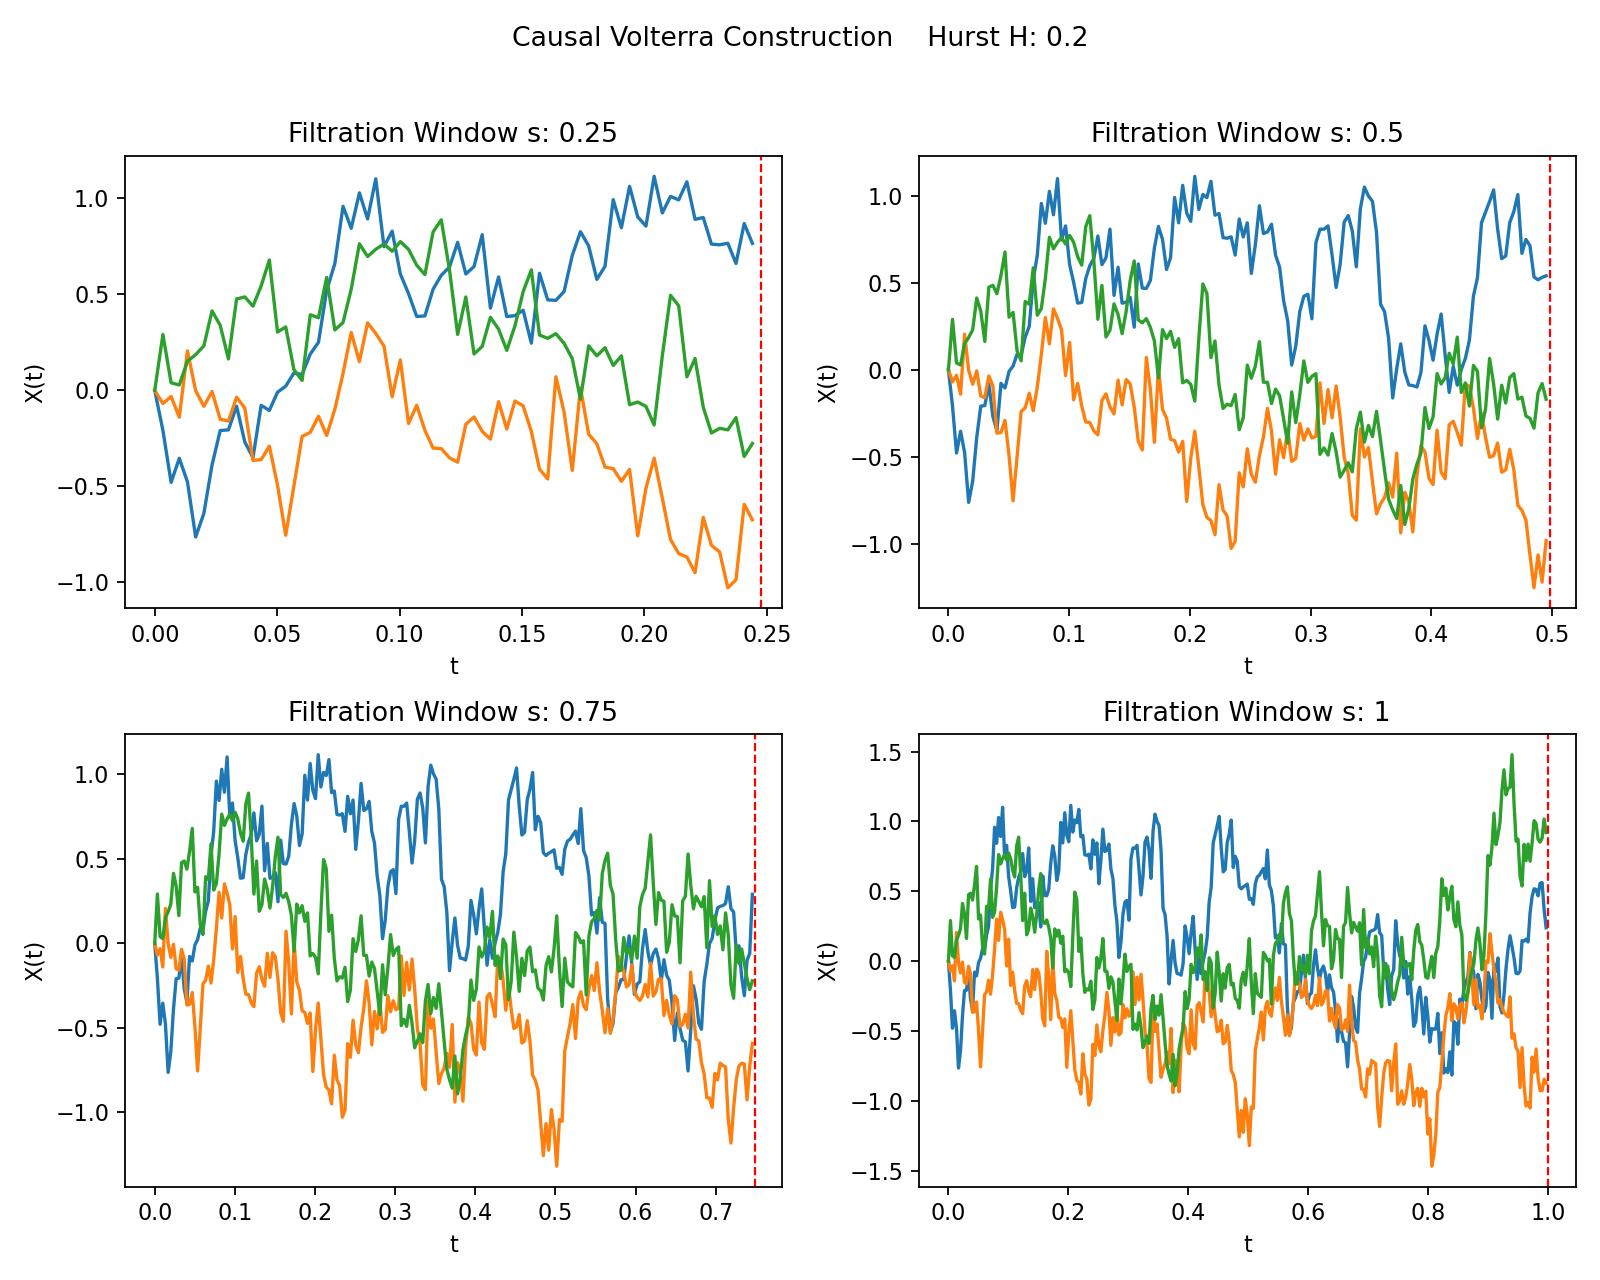
\includegraphics[width=\linewidth]{img/revisionato/2/iterative0.2.png}
\end{minipage}
\hfill
\begin{minipage}[t]{0.52\textwidth}
\vspace{0pt}
\centering
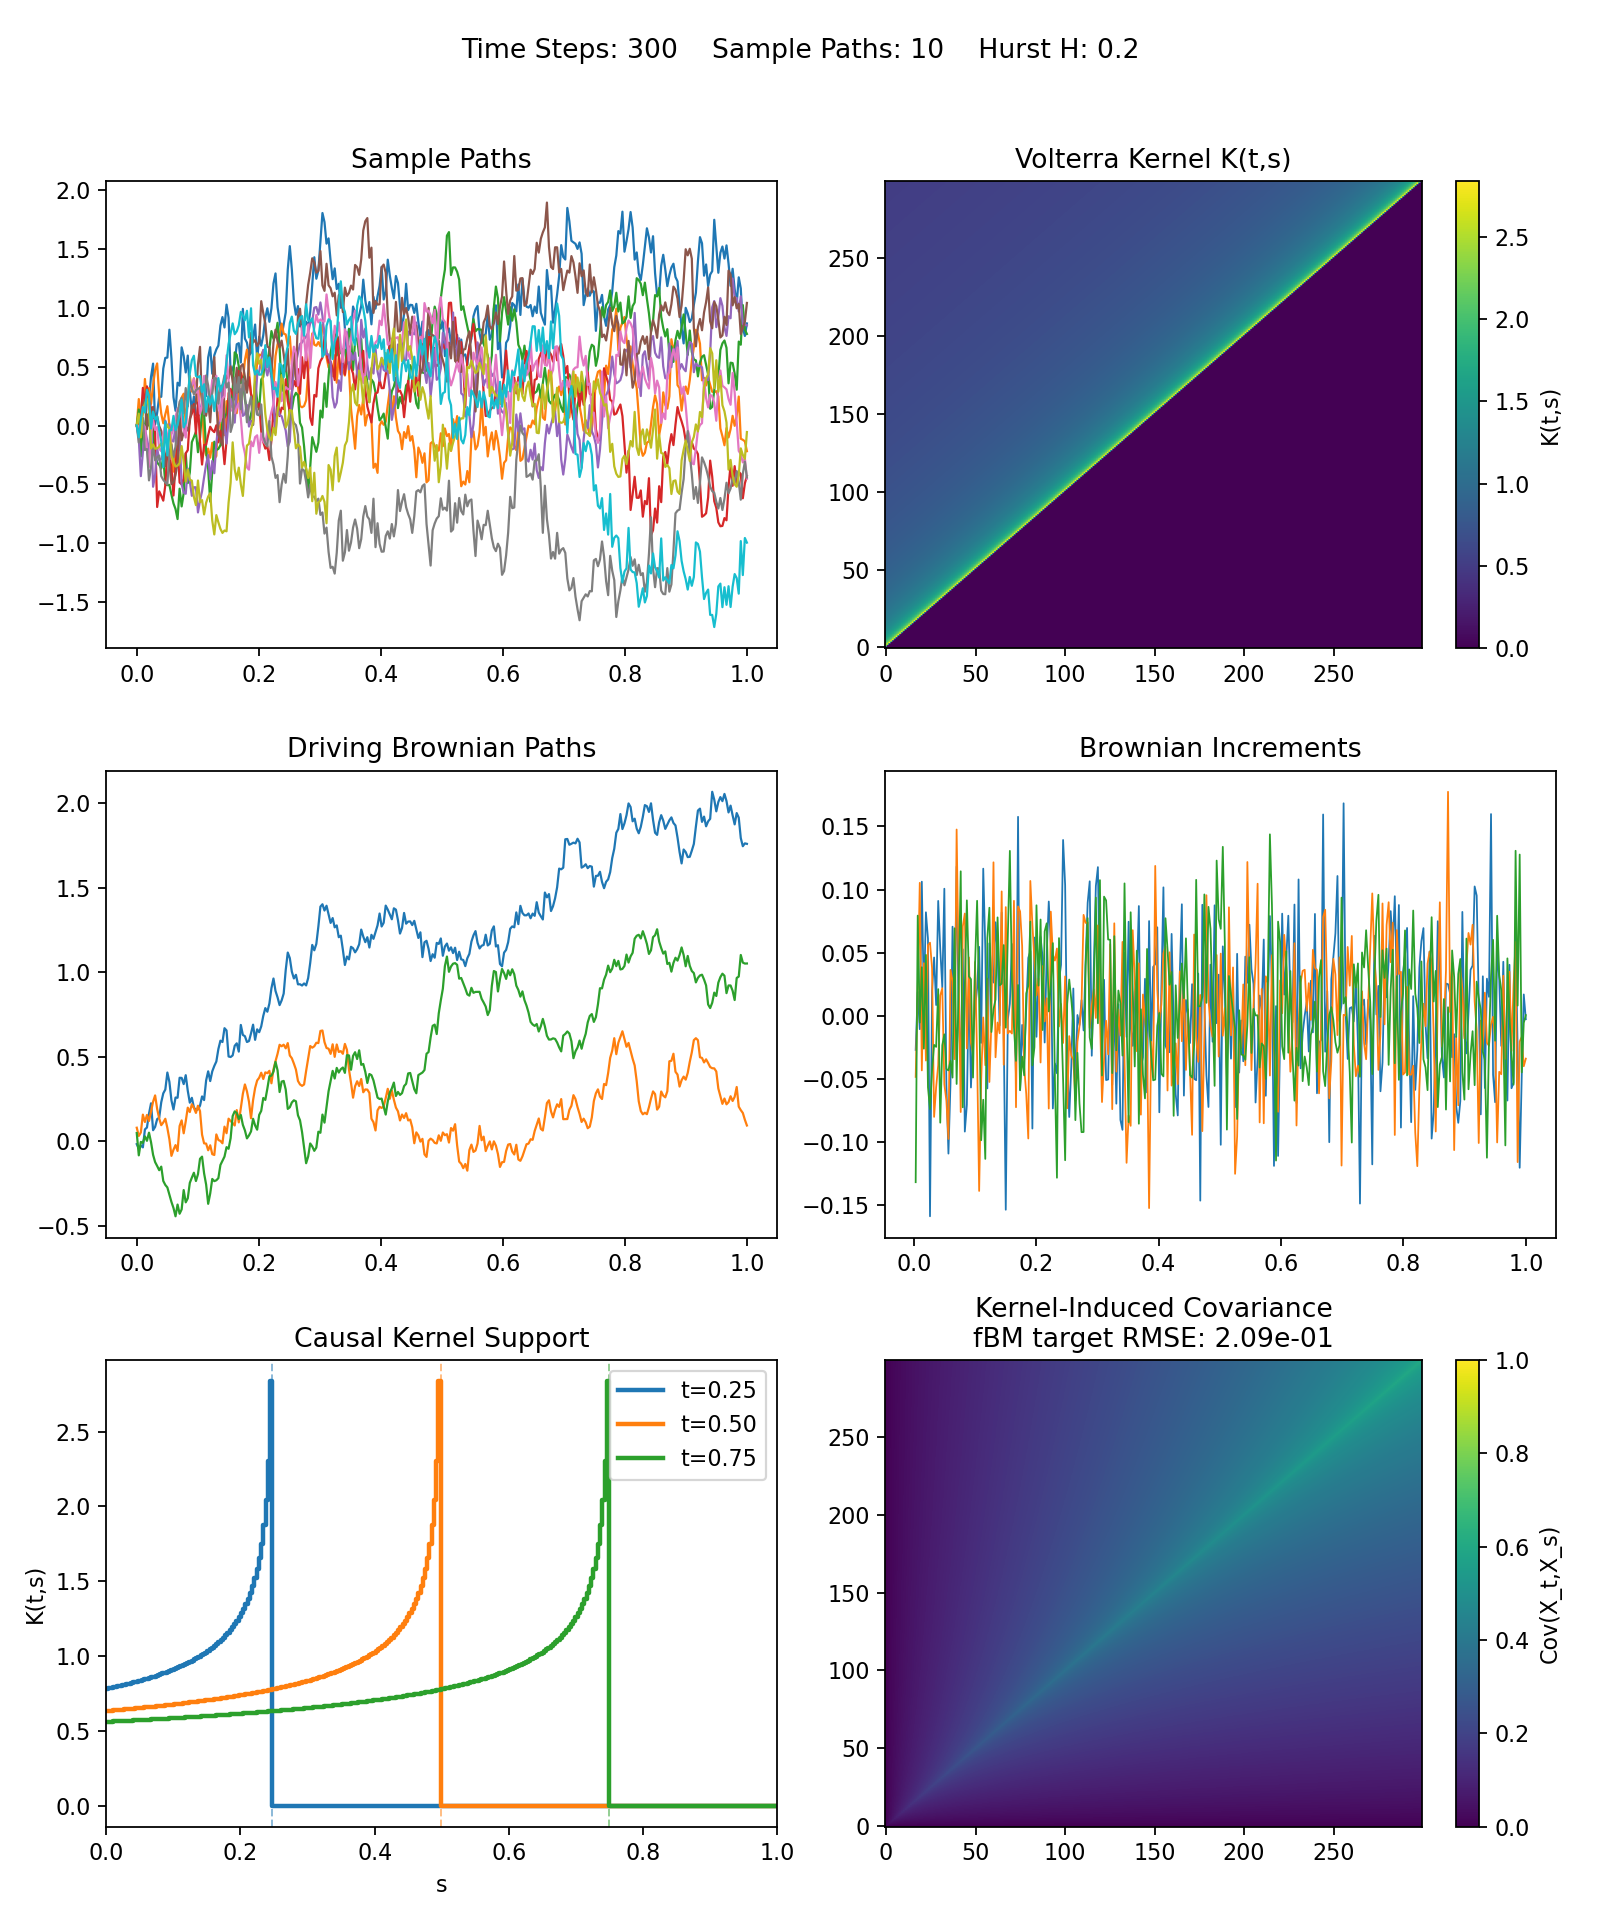
\includegraphics[width=\linewidth]{img/revisionato/2/volterra0.2.png}
\end{minipage}
\end{figure}

\begin{figure}[H]
\centering
\begin{minipage}[t]{0.52\textwidth}
\vspace{0.4cm}
\centering
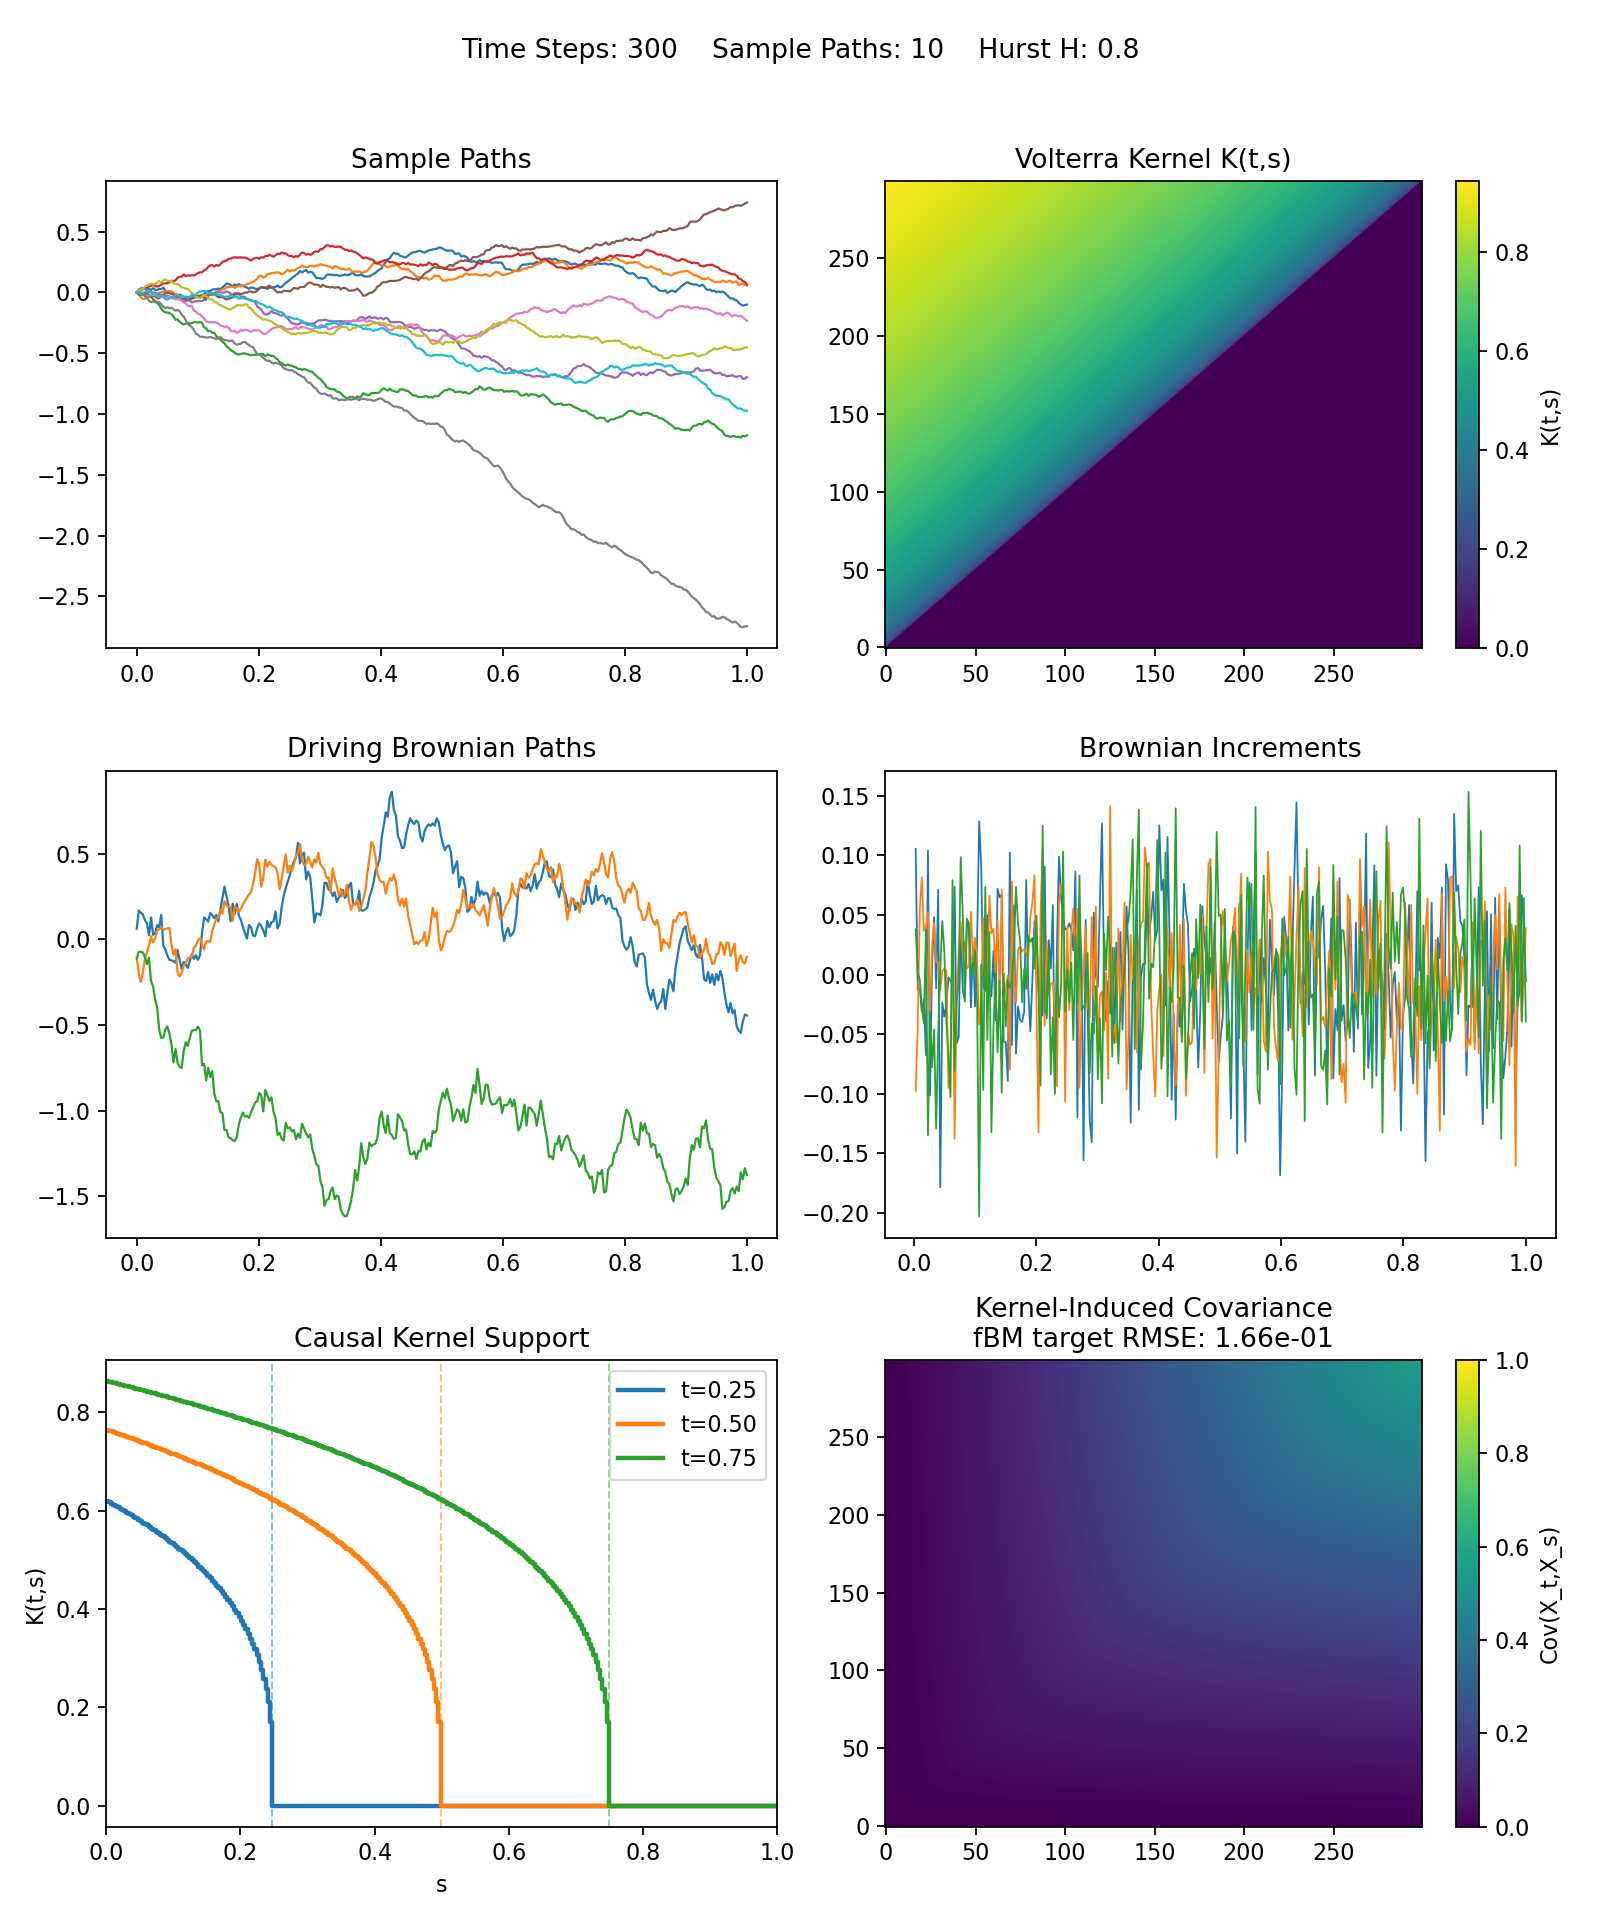
\includegraphics[width=\linewidth]{img/revisionato/2/volterra0.8.png}
\end{minipage}
\hfill
\begin{minipage}[t]{0.42\textwidth}
\vspace{0pt}
\normalsize


\textbf{Persistent regime: \(H=0.8\).}

When \(H>\tfrac12\), the kernel becomes smoother and the relative importance of more distant history increases. The process still has a causal representation, since only past noise is used, but the accumulated effect of history now produces much smoother and more persistent trajectories. This is visible both in the iterative construction and in the full Volterra diagnostics: the paths display stronger directional continuity, and the covariance pattern becomes more persistent across time indices.

\vspace{0.5cm}
\centering
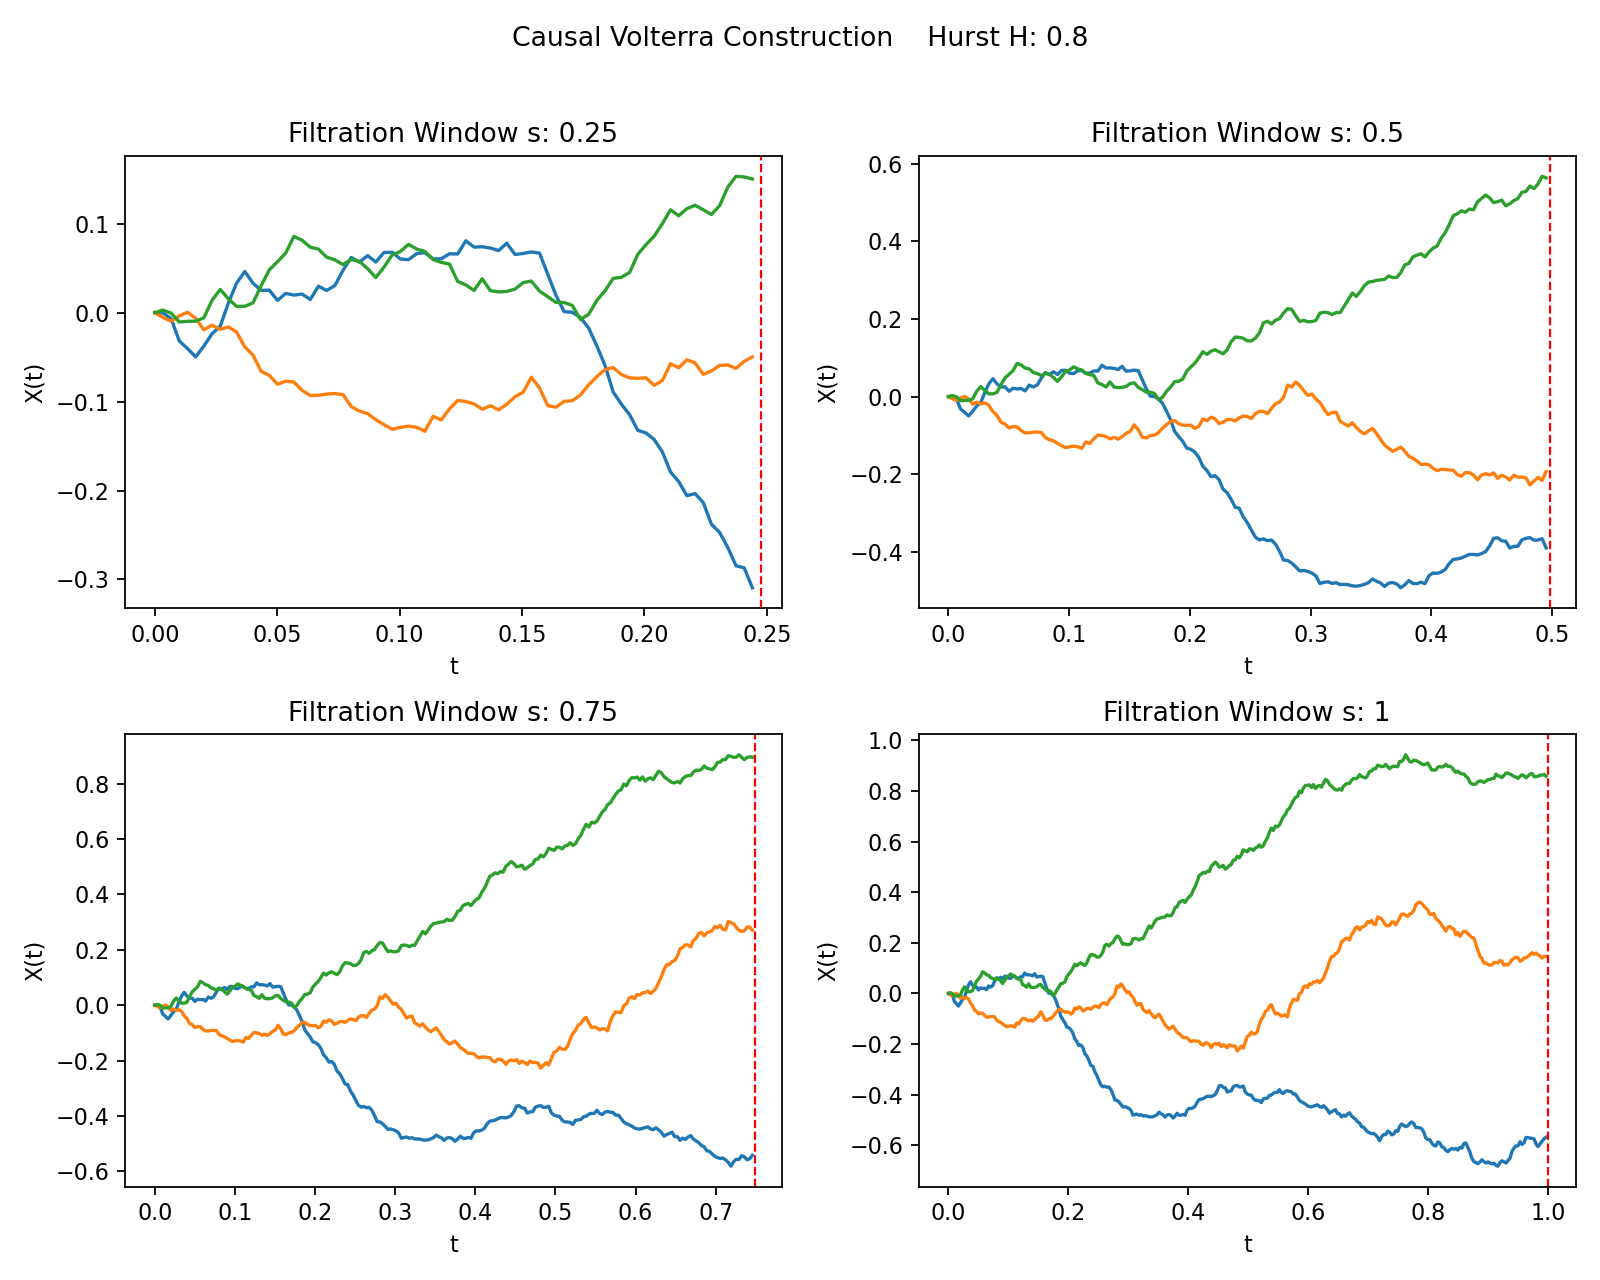
\includegraphics[width=\linewidth]{img/revisionato/2/iterative0.8.png}
\end{minipage}
\end{figure}
\clearpage
\paragraph{Implementation.}

A convenient way to simulate a Volterra process numerically is to implement a generic routine that accepts a kernel as an argument. This makes it possible to recover Brownian motion, Ornstein--Uhlenbeck dynamics, or fractional-type processes simply by changing the kernel.

This implementation is intentionally generic. If one calls the simulator with \texttt{brownian\_kernel}, the output is a Brownian path written in Volterra form. If one uses \texttt{ou\_kernel(theta)}, the output becomes an Ornstein--Uhlenbeck process. If one uses \texttt{fractional\_kernel(H)}, the output is a causal fractional-type Volterra process whose roughness and persistence are controlled by \(H\).

\paragraph{Computational cost and transition to lifting.}

The Volterra representation solves the causality problem, but it does not eliminate the memory problem. To compute \(X_{t_i}\), one still has to survey the entire history of shocks \(\Delta W_0,\dots,\Delta W_{i-1}\). As a consequence, the cost per path grows roughly quadratically in the number of time steps:
\[
\text{cost per path} \sim O(n^2).
\]
This is acceptable for a theoretical laboratory and for moderate Monte Carlo experiments, but it becomes expensive once the process is embedded inside calibration loops, filtering procedures, or control problems.

The important gain is therefore structural rather than asymptotic: Volterra processes are causal, interpretable, and directly suited to sequential simulation. Their remaining computational bottleneck is exactly what motivates the next step of the paper. If the kernel can be approximated by a finite mixture of exponentials, the process can be rewritten in an enlarged but finite-dimensional Markovian state space. This is the idea behind Markovian lifting, which preserves the rough-memory intuition while recovering a tractable recursive structure for simulation and control.

%%%%%%%%%%%%%%%%%%%%%%%%%%%%%%%%%%%%%%%%%%%%%%%%
%%%%%%%%%%%%%%%%%%%%%%%%%%%%%%%%%%%%%%%%%%%%%%%%
%%%%%%%%%%%%%%%%%%%%%%%%%%%%%%%%%%%%%%%%%%%%%%%%

\chapter{Markovian Lifting}
\miniabstract{The previous chapter made rough dynamics causal through Volterra kernels, but each update still carried the whole history of past shocks. This chapter addresses that bottleneck by approximating the rough kernel with a finite mixture of exponentials, turning path-dependent memory into a finite-dimensional Markov state for recursive simulation, calibration, and control.}

\paragraph{Why lifting is needed.}

A Markov process has the property that the future depends on the present state alone. This is precisely what makes Brownian-motion-based models so efficient computationally: when one wants to generate the next step of the path, the whole history is not needed. By contrast, rough and fractional models are designed to preserve memory. In a Volterra representation,
\[
X_t=\int_0^t K(t,s)\,dW_s,
\]
the kernel \(K\) makes the current state depend on the entire past trajectory of the driving noise. This is mathematically attractive, but it destroys the simple recursive structure that is available in a Markov model.

One could always make the path itself part of the state, but that would not really solve anything. Expanding the state space to include the entire history is exact, yet it is not a simplification. The idea of Markovian lifting is more selective: instead of keeping the full path, one approximates the effect of the path by a finite collection of auxiliary state variables that are themselves Markovian. In this way, one retains the main covariance features of the rough dynamics without carrying the full historical trajectory at every step.

\section{Why exponentials are special}

The key mathematical reason lifting works is that exponentials satisfy a semigroup property. For any \(x>0\),
\[
e^{-x(t+\Delta t-s)} = e^{-x\Delta t}e^{-x(t-s)}.
\]
This simple identity is enough to recover a Markov recursion. To see it, define for a fixed rate \(x>0\) the auxiliary process
\[
U_t(x)=\int_0^t e^{-x(t-s)}\,dW_s.
\]
Then
\[
U_{t+\Delta t}(x)
=
\int_0^{t+\Delta t} e^{-x(t+\Delta t-s)}\,dW_s.
\]
Splitting the integral at time \(t\) and applying the semigroup property gives
\[
U_{t+\Delta t}(x)
=
e^{-x\Delta t}\int_0^t e^{-x(t-s)}\,dW_s
+
\int_t^{t+\Delta t} e^{-x(t+\Delta t-s)}\,dW_s,
\]
hence
\[
U_{t+\Delta t}(x)
=
e^{-x\Delta t}U_t(x)
+
\int_t^{t+\Delta t} e^{-x(t+\Delta t-s)}\,dW_s.
\]
The first term depends only on the current state \(U_t(x)\), while the second term depends only on the new Brownian increment over \([t,t+\Delta t]\). This is exactly the structure of a Markov update.

This mechanism fails for a pure power law. If one considers a rough kernel of the form
\[
(t-s)^{\alpha-1},
\]
then in general
\[
(t+\Delta t-s)^{\alpha-1}
\neq
(\Delta t)^{\alpha-1}(t-s)^{\alpha-1}.
\]
The semigroup property is absent, and this is the algebraic reason why pure rough kernels remain non-Markovian.

\section{Laplace representation of the rough kernel}

The rough-volatility kernel is typically written in the power-law form
\[
K_\alpha(\tau)=\frac{\tau^{\alpha-1}}{\Gamma(\alpha)},
\qquad
\alpha\in\left(\frac12,1\right),
\qquad
\tau>0.
\]
If one writes \(\alpha=H+\tfrac12\), then the rough regime corresponds to \(H\in(0,\tfrac12)\). The key observation behind lifting is that this kernel can be represented as a Laplace transform of exponential functions.

\begin{proposition}[Laplace representation of the power-law kernel]
For \(\alpha\in(0,1)\) and \(\tau>0\),
\[
\frac{\tau^{\alpha-1}}{\Gamma(\alpha)}
=
\frac{1}{\Gamma(\alpha)\Gamma(1-\alpha)}
\int_0^\infty e^{-\lambda \tau}\lambda^{-\alpha}\,d\lambda.
\]
Using Euler's reflection formula,
\[
\frac{1}{\Gamma(\alpha)\Gamma(1-\alpha)}
=
\frac{\sin(\pi\alpha)}{\pi},
\]
so equivalently
\[
\frac{\tau^{\alpha-1}}{\Gamma(\alpha)}
=
\frac{\sin(\pi\alpha)}{\pi}
\int_0^\infty e^{-\lambda \tau}\lambda^{-\alpha}\,d\lambda.
\]
\end{proposition}

\begin{proof}
By definition of the Gamma function,
\[
\Gamma(1-\alpha)=\int_0^\infty u^{-\alpha}e^{-u}\,du.
\]
Now make the substitution \(u=\lambda \tau\), so that \(du=\tau\,d\lambda\). Then
\[
\Gamma(1-\alpha)
=
\int_0^\infty (\lambda\tau)^{-\alpha}e^{-\lambda\tau}\tau\,d\lambda
=
\tau^{1-\alpha}\int_0^\infty \lambda^{-\alpha}e^{-\lambda\tau}\,d\lambda.
\]
Dividing both sides by \(\tau^{1-\alpha}\Gamma(\alpha)\Gamma(1-\alpha)\) gives
\[
\frac{\tau^{\alpha-1}}{\Gamma(\alpha)}
=
\frac{1}{\Gamma(\alpha)\Gamma(1-\alpha)}
\int_0^\infty e^{-\lambda\tau}\lambda^{-\alpha}\,d\lambda.
\qedhere
\]
\end{proof}

This identity is the analytical foundation of Markovian lifting. A singular power-law kernel can be interpreted as a continuous mixture of exponential kernels, and each exponential kernel corresponds to one mean-reverting Markov factor.

\section{From a continuous mixture to a finite lifted state}

The continuous Laplace representation is still infinite-dimensional. To obtain a practical model, one replaces the integral over \(\lambda\) by a finite quadrature rule. Choose rates
\[
\lambda_1,\dots,\lambda_M>0
\]
and positive weights
\[
w_1,\dots,w_M>0.
\]
Then approximate the rough kernel by
\[
K_\alpha(\tau)\approx K_\alpha^{(M)}(\tau)
=
\sum_{k=1}^M w_k e^{-\lambda_k \tau}.
\]
The corresponding lifted process becomes
\[
Y_t^{(M)}
=
\int_0^t K_\alpha^{(M)}(t-s)\,dW_s
=
\sum_{k=1}^M w_k U_t^{(k)},
\]
where
\[
U_t^{(k)}
=
\int_0^t e^{-\lambda_k(t-s)}\,dW_s.
\]
Each factor \(U^{(k)}\) is an Ornstein--Uhlenbeck-type Gaussian state satisfying
\[
dU_t^{(k)}=-\lambda_k U_t^{(k)}\,dt + dW_t,
\qquad
U_0^{(k)}=0.
\]
The entire lifted state is therefore
\[
Z_t=\bigl(U_t^{(1)},\dots,U_t^{(M)}\bigr)^\top,
\]
which is finite-dimensional and Markovian.

This is the core idea of lifting: instead of carrying an infinite-dimensional Volterra memory, one works with a stack of \(M\) mean-reverting factors. The model is no longer exact at finite \(M\), but it regains the recursive structure that is lost in the rough Volterra formulation.

\paragraph{Why this matters for rough volatility.}

The relevance of lifting is especially clear in rough-volatility models. A prototypical rough variance process may be written schematically as
\[
V_t
=
V_0
+
\int_0^t K_\alpha(t-s)\,dZ_s,
\]
where \(Z\) collects the drift and volatility-of-volatility terms. The non-Markovian difficulty comes entirely from the kernel \(K_\alpha\). Once \(K_\alpha\) is replaced by its finite exponential approximation \(K_\alpha^{(M)}\), the same variance process can be written as a linear combination of \(M\) Markovian factors:
\[
V_t
\approx
V_0+\sum_{k=1}^M w_k U_t^{(k)}.
\]
This is the step that restores the affine-type structure and makes fast simulation feasible again. In other words, lifting does not eliminate roughness by ignoring it; it replaces roughness by a structured finite-dimensional approximation that can still be handled recursively.

\section{Discrete-time recursion}

Fix a uniform grid
\[
t_i=i\Delta t,
\qquad i=0,\dots,n,
\qquad \Delta t=\frac{T}{n}.
\]
For each OU factor, the exact one-step transition is
\[
U_{i+1}^{(k)}=e^{-\lambda_k\Delta t}U_i^{(k)}+\eta_{i+1}^{(k)},
\]
where the innovation vector
\[
\eta_{i+1}=
\bigl(\eta_{i+1}^{(1)},\dots,\eta_{i+1}^{(M)}\bigr)^\top
\]
is centered Gaussian. Because all factors are driven by the same Brownian motion, these innovations are correlated, with covariance
\[
\Cov\!\bigl(\eta^{(j)},\eta^{(k)}\bigr)
=
\frac{1-e^{-(\lambda_j+\lambda_k)\Delta t}}{\lambda_j+\lambda_k}.
\]
After updating the factors, the lifted process is reconstructed by
\[
Y_i^{(M)}=\sum_{k=1}^M w_k U_i^{(k)}.
\]

An equivalent weighted-state representation is also possible. One may define
\[
X_t^{(k)}:=w_k U_t^{(k)},
\]
so that
\[
dX_t^{(k)}=-\lambda_k X_t^{(k)}\,dt+w_k\,dW_t,
\qquad
Y_t^{(M)}=\sum_{k=1}^M X_t^{(k)}.
\]
In that convention, the innovation covariance becomes
\[
\Cov\!\bigl(\eta^{(j)},\eta^{(k)}\bigr)
=
w_jw_k\,
\frac{1-e^{-(\lambda_j+\lambda_k)\Delta t}}{\lambda_j+\lambda_k}.
\]
Both formulations are equivalent as long as the weights are used consistently.

\section{Practical construction of the lift}

\paragraph{Rates and weights.}

The finite approximation depends on the choice of quadrature nodes \(\lambda_k\) and weights \(w_k\). A common practical heuristic is to use log-spaced rates,
\[
\lambda_k \in \left[\frac{2}{T},\frac{400}{T}\right],
\]
and weights proportional to
\[
w_k \propto \lambda_k^{-(H+\frac12)}.
\]
This mirrors the Laplace-domain mass of the rough kernel and usually provides a reasonable first approximation. However, this choice is heuristic rather than optimal. In particular, the approximation error is not guaranteed to decrease monotonically with \(M\), and in finite samples the empirical covariance RMSE may oscillate because of three interacting effects:
\begin{itemize}
    \item approximation error from the finite exponential mixture,
    \item Monte Carlo noise from the simulated covariance matrix,
    \item numerical conditioning effects when the factor system becomes larger.
\end{itemize}

For this reason, one should interpret the lifting dimension \(M\) as a bias--variance trade-off rather than as a parameter for which ``larger is always better''. In practice, a moderate value often gives the most stable overall result.

\paragraph{Discrete-time recipe.}

A convenient summary of the lifting procedure is the following:

\begin{enumerate}[label=\arabic*.]
    \item Choose a Hurst parameter \(H\in(0,1)\) and a lifting dimension \(M\).
    \item Define a time grid \(t_i=i\Delta t\) on \([0,T]\).
    \item Select mean-reversion rates \(\lambda_1,\dots,\lambda_M\), typically on a log scale.
    \item Choose weights \(w_1,\dots,w_M\) from a Laplace-domain quadrature heuristic.
    \item Build the Gaussian innovation covariance matrix of the OU factors.
    \item Simulate the factor recursion
    \[
    U_{i+1}^{(k)}=e^{-\lambda_k\Delta t}U_i^{(k)}+\eta_{i+1}^{(k)}.
    \]
    \item Aggregate the factors through
    \[
    Y_i^{(M)}=\sum_{k=1}^M w_k U_i^{(k)}.
    \]
\end{enumerate}

When the objective is to compare the lifted process directly with fractional Brownian motion on a fixed grid, it is often useful to rescale each time column so that the marginal variance matches
\[
\Var(B_t^H)=t^{2H}.
\]
This does not turn the lift into exact fractional Brownian motion. It simply isolates the covariance-shape approximation from a mismatch in marginal scale.

\paragraph{Implementation.}

This implementation keeps the OU factors unweighted internally and applies the weights only at aggregation. The function \texttt{match\_fbm\_marginals} can then be used when the goal is a direct visual or covariance comparison with fractional Brownian motion on a fixed discrete grid.

\section{Visual comparison across Hurst parameters}

The panels below illustrate the lifted approximation for three representative values of the Hurst parameter. In each composite image, the main lifted covariance is shown together with the target fractional covariance and a lag-wise covariance-error profile. The smaller diagnostic panels also compare nearby lifting dimensions, which makes it possible to see that the empirical error does not necessarily decrease monotonically as the number of OU factors changes.

The important point is therefore not a perfectly monotone RMSE sequence, but rather the overall stability of the approximation. Across repeated simulations, the empirical covariance error oscillates because it is itself a Monte Carlo object. 

The case $H=0.8$ is included as a persistent stress regime for the numerical comparison. It lies outside the standard empirically rough range $H<\tfrac12$ covered by the singular-kernel argument above, so it should not be read as a claim that persistent volatility is rough in the usual sense.

\begin{algorithm}[H]
\caption{Reading the Markovian-lifting diagnostic panels}
\DontPrintSemicolon
choose \(H\), a factor count \(M\), rates \(\lambda_k\), and weights \(w_k\)\;
simulate the correlated OU-factor recursion for the lifted state\;
aggregate \(Y^{(M)}=\sum_k w_k U^{(k)}\) and match the marginal scale when comparing with \(B^H\)\;
estimate the lifted covariance, compare it with the fractional target, and plot the lag-wise error\;
\end{algorithm}

Nevertheless, the error remains controlled, the qualitative geometry of the covariance surface is preserved, and the lift continues to reproduce the broad persistence pattern of the target process. In particular, the roughest regime is the hardest one to approximate, while smoother regimes are matched more easily.

\begin{figure}[H]
\centering
\begin{minipage}[t]{0.47\textwidth}
\vspace{0pt}
\normalsize

\vspace{0.25cm}

\textbf{Benchmark regime: \(H=0.5\).}

This is the intermediate benchmark case. The lifted covariance already captures the broad triangular structure of the target fractional covariance, but the lag-wise error profile shows that the approximation is still imperfect. The nearby factor-count diagnostics included in the panel also illustrate a practical point: changing the number of OU factors does not produce a strictly monotone reduction of the empirical RMSE. In repeated runs, the error oscillates because approximation error and Monte Carlo noise interact, but it remains controlled and the overall covariance geometry is preserved.

\end{minipage}
\hfill
\begin{minipage}[t]{0.47\textwidth}
\vspace{0pt}
\centering
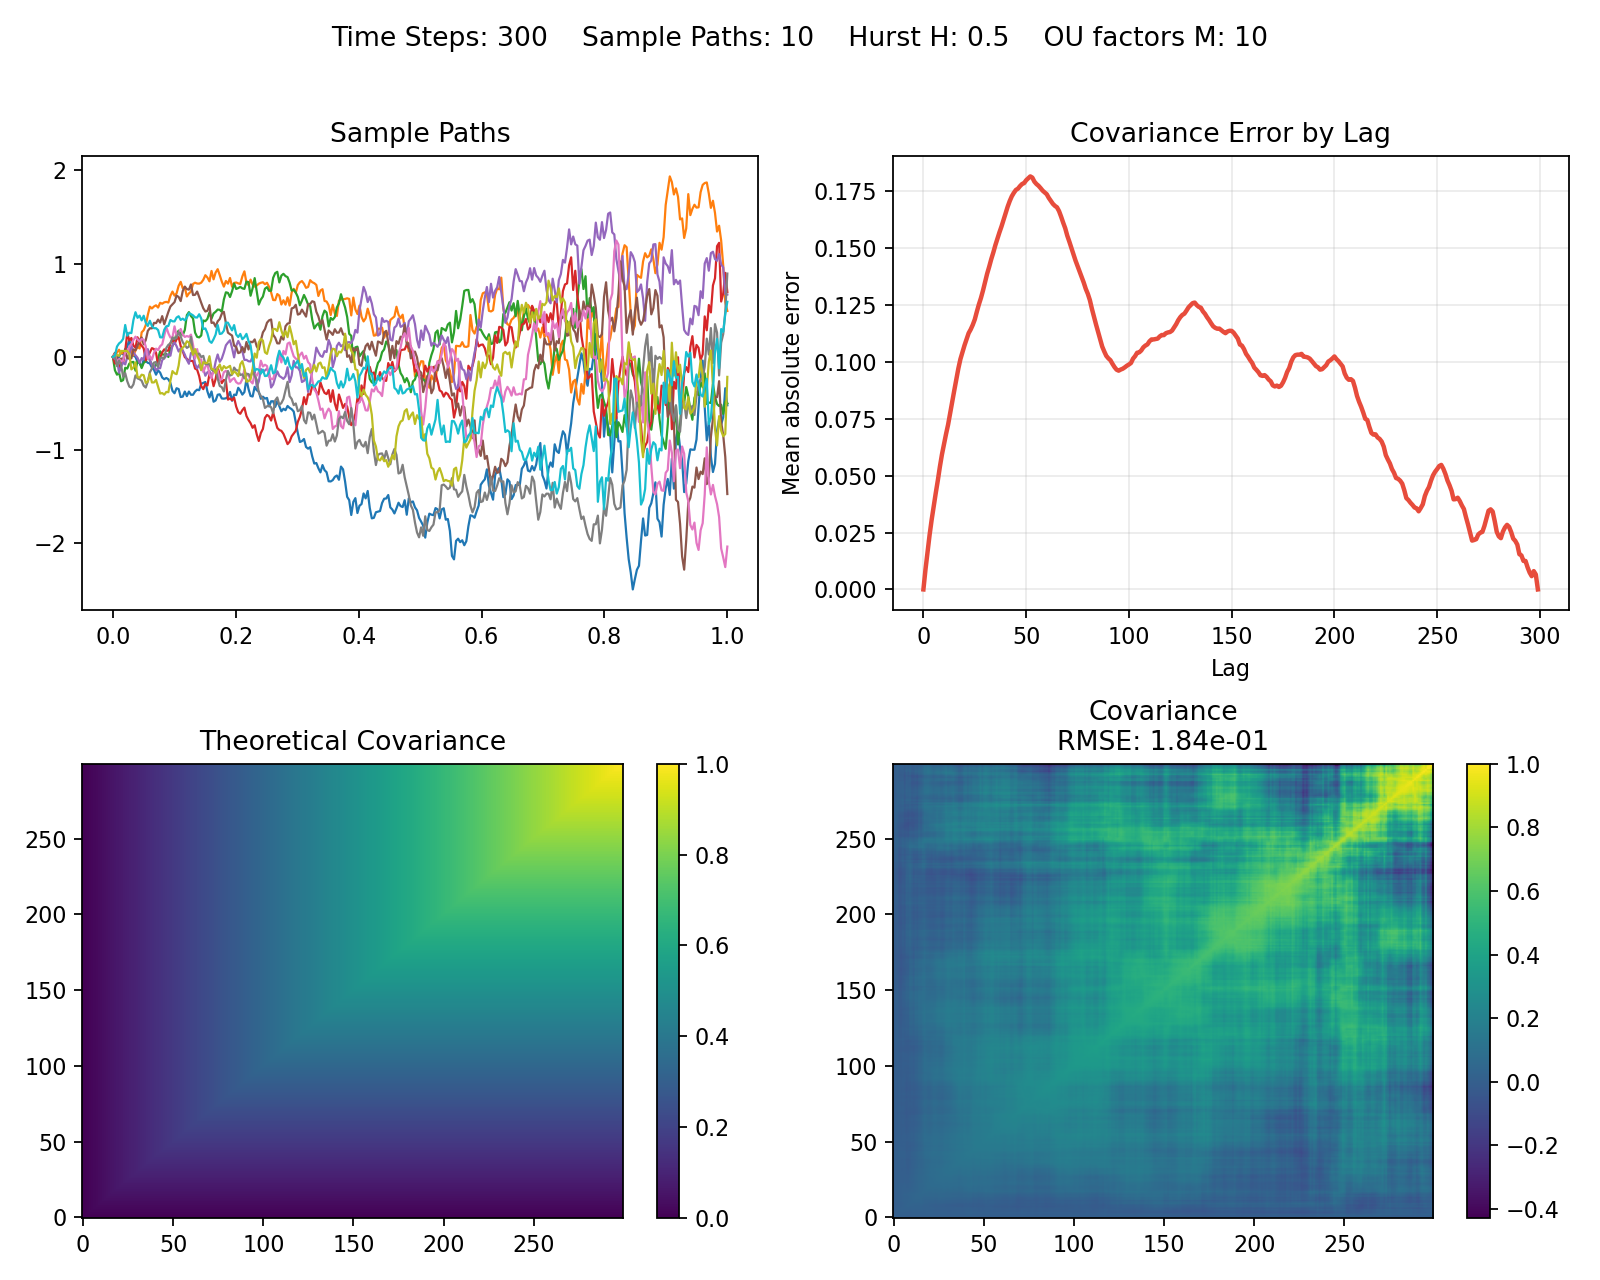
\includegraphics[width=6.5cm]{img/revisionato/2/ML0.5.png}
\end{minipage}
\end{figure}

\begin{figure}[H]
\centering
\begin{minipage}[t]{0.47\textwidth}
\vspace{0pt}
\centering
%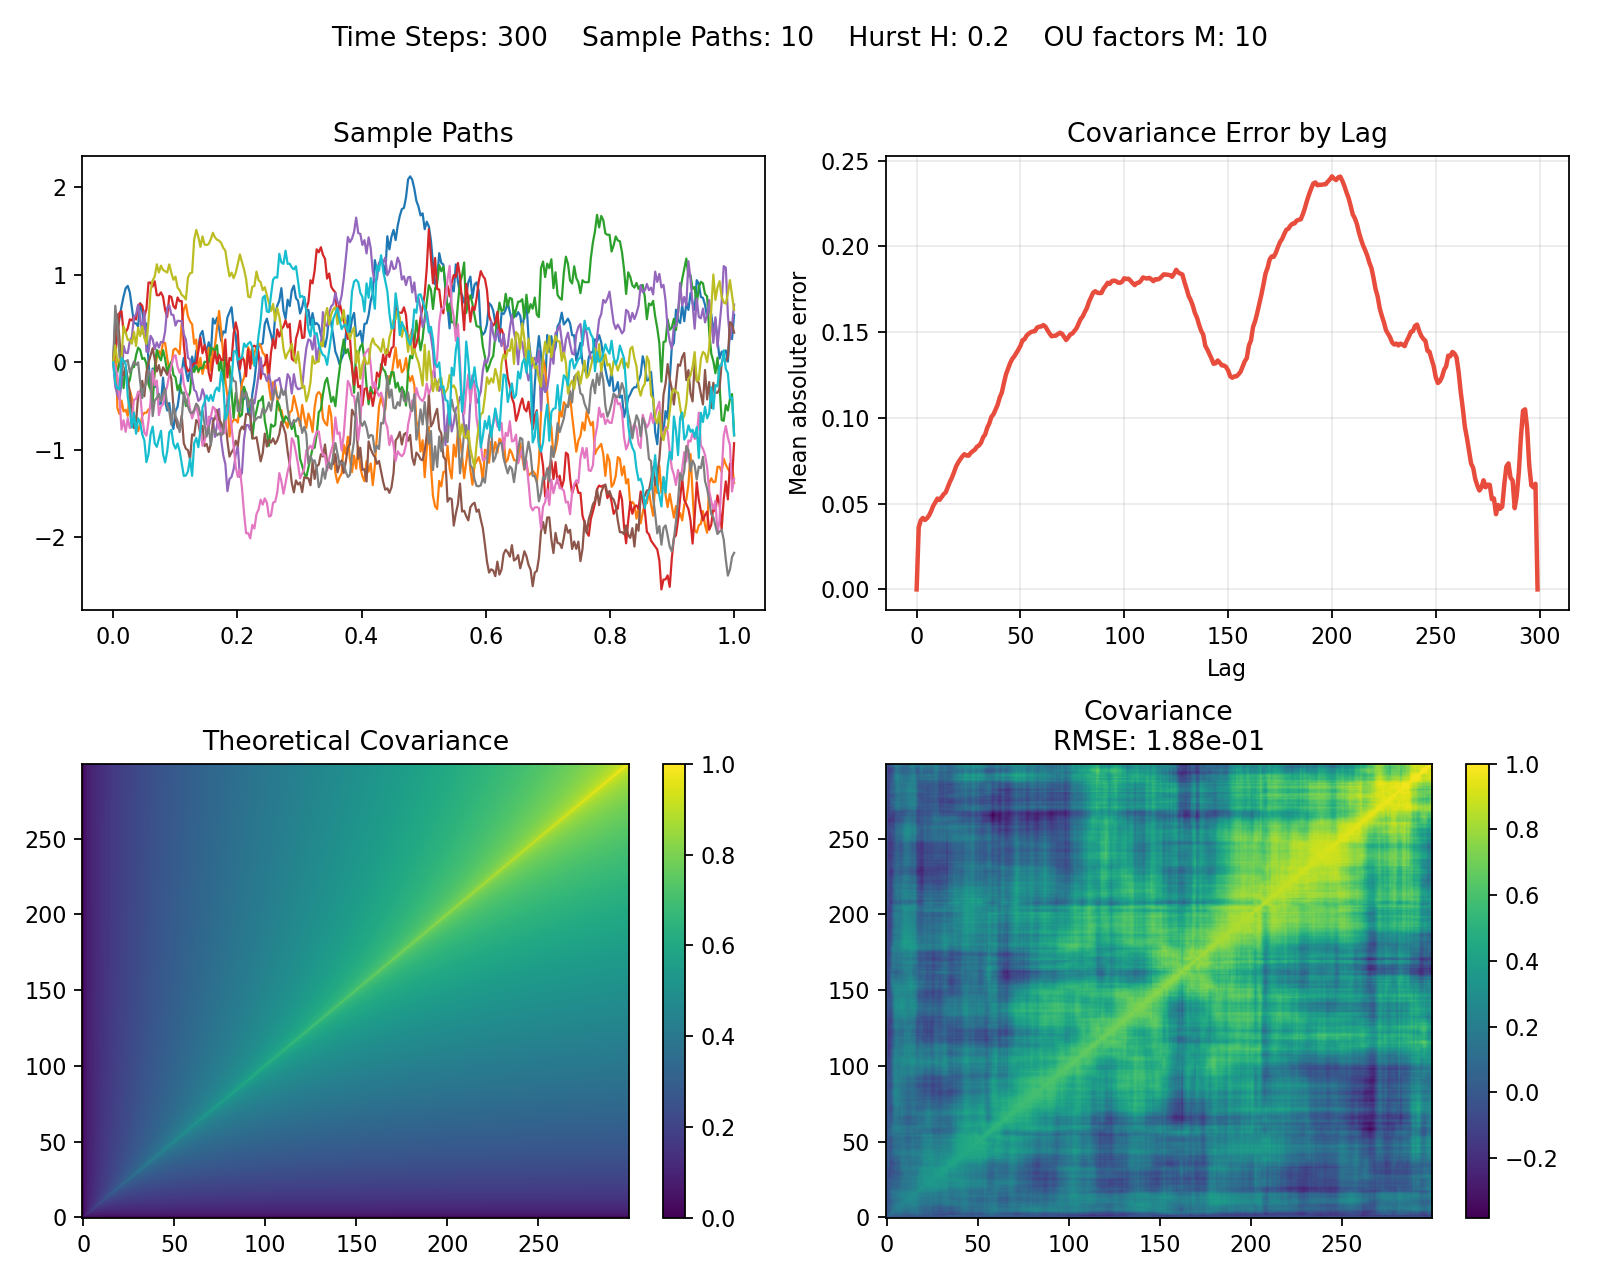
\includegraphics[width=\linewidth]{img/revisionato/2/ML0.2.png}
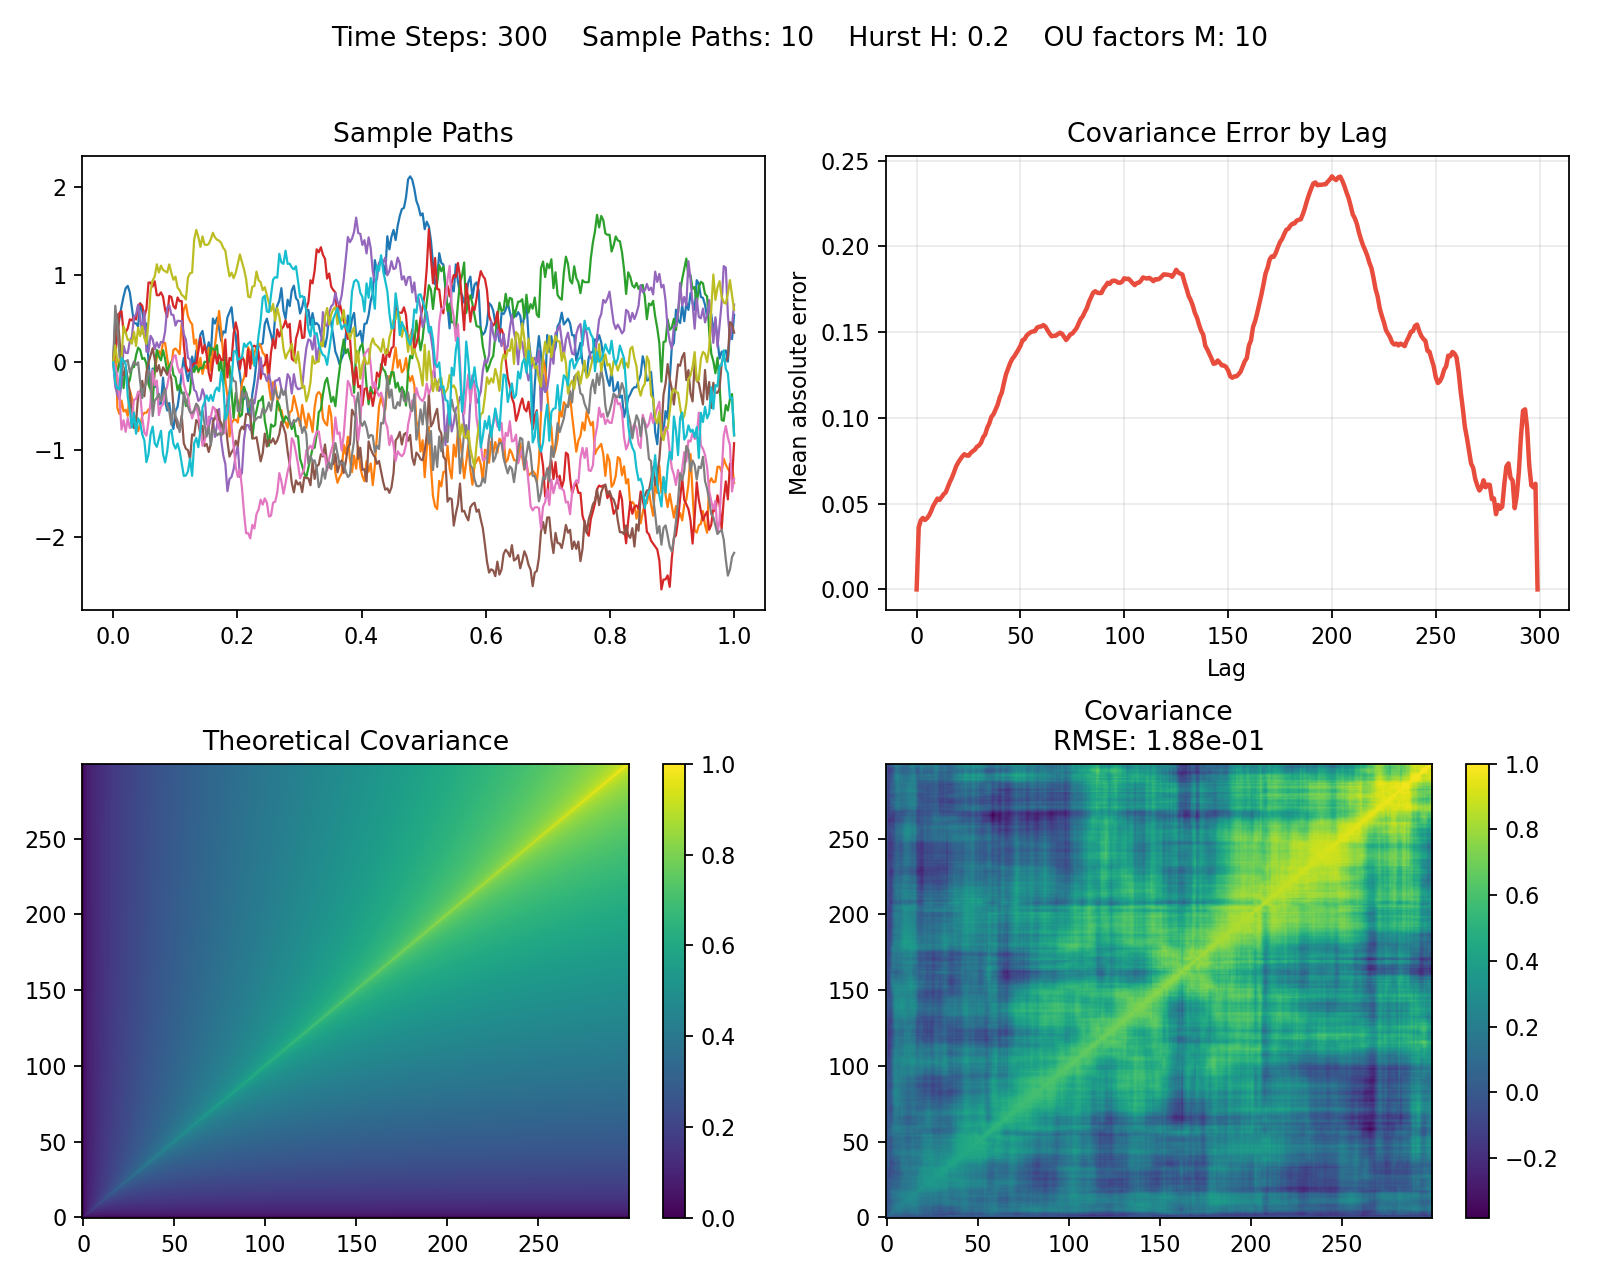
\includegraphics[width=6.5cm]{img/revisionato/2/ML0.2.png}
\end{minipage}
\hfill
\begin{minipage}[t]{0.47\textwidth}
\vspace{0pt}
\normalsize
\textbf{Rough regime: \(H=0.2\).}

This is the most challenging case. Because the target covariance is generated by a much rougher kernel, a finite exponential mixture has a harder task: the lifted approximation still reproduces the global covariance pattern, but the empirical RMSE is larger and the lag-wise error is more pronounced. This should not be interpreted as a failure of the method. Rather, it shows that the roughest regime is the one in which the finite-dimensional approximation is under the greatest pressure. Even here, however, repeated simulation does not produce unstable behavior: %the error fluctuates from run to run, but remains bounded and the target covariance shape is still clearly recognizable.
\end{minipage}
\end{figure}

the error fluctuates from run to run, but remains bounded and the target covariance shape is still clearly recognizable.

\begin{figure}[H]
\centering
\begin{minipage}[t]{0.47\textwidth}
\vspace{0.25cm}
\normalsize
\textbf{Persistent regime: \(H=0.8\).}

When \(H>\tfrac12\), the target covariance is smoother and the lifted approximation becomes noticeably easier. This is reflected both in the heat maps and in the much smaller lag-wise covariance error. In this regime the exponential mixture is already rich enough to track the target geometry rather closely. As before, the RMSE observed in simulation is not perfectly deterministic across runs, but its oscillations remain small and the approximation is visibly more accurate than in the rough case.


\end{minipage}
\hfill
\begin{minipage}[t]{0.47\textwidth}
\vspace{0pt}
\centering
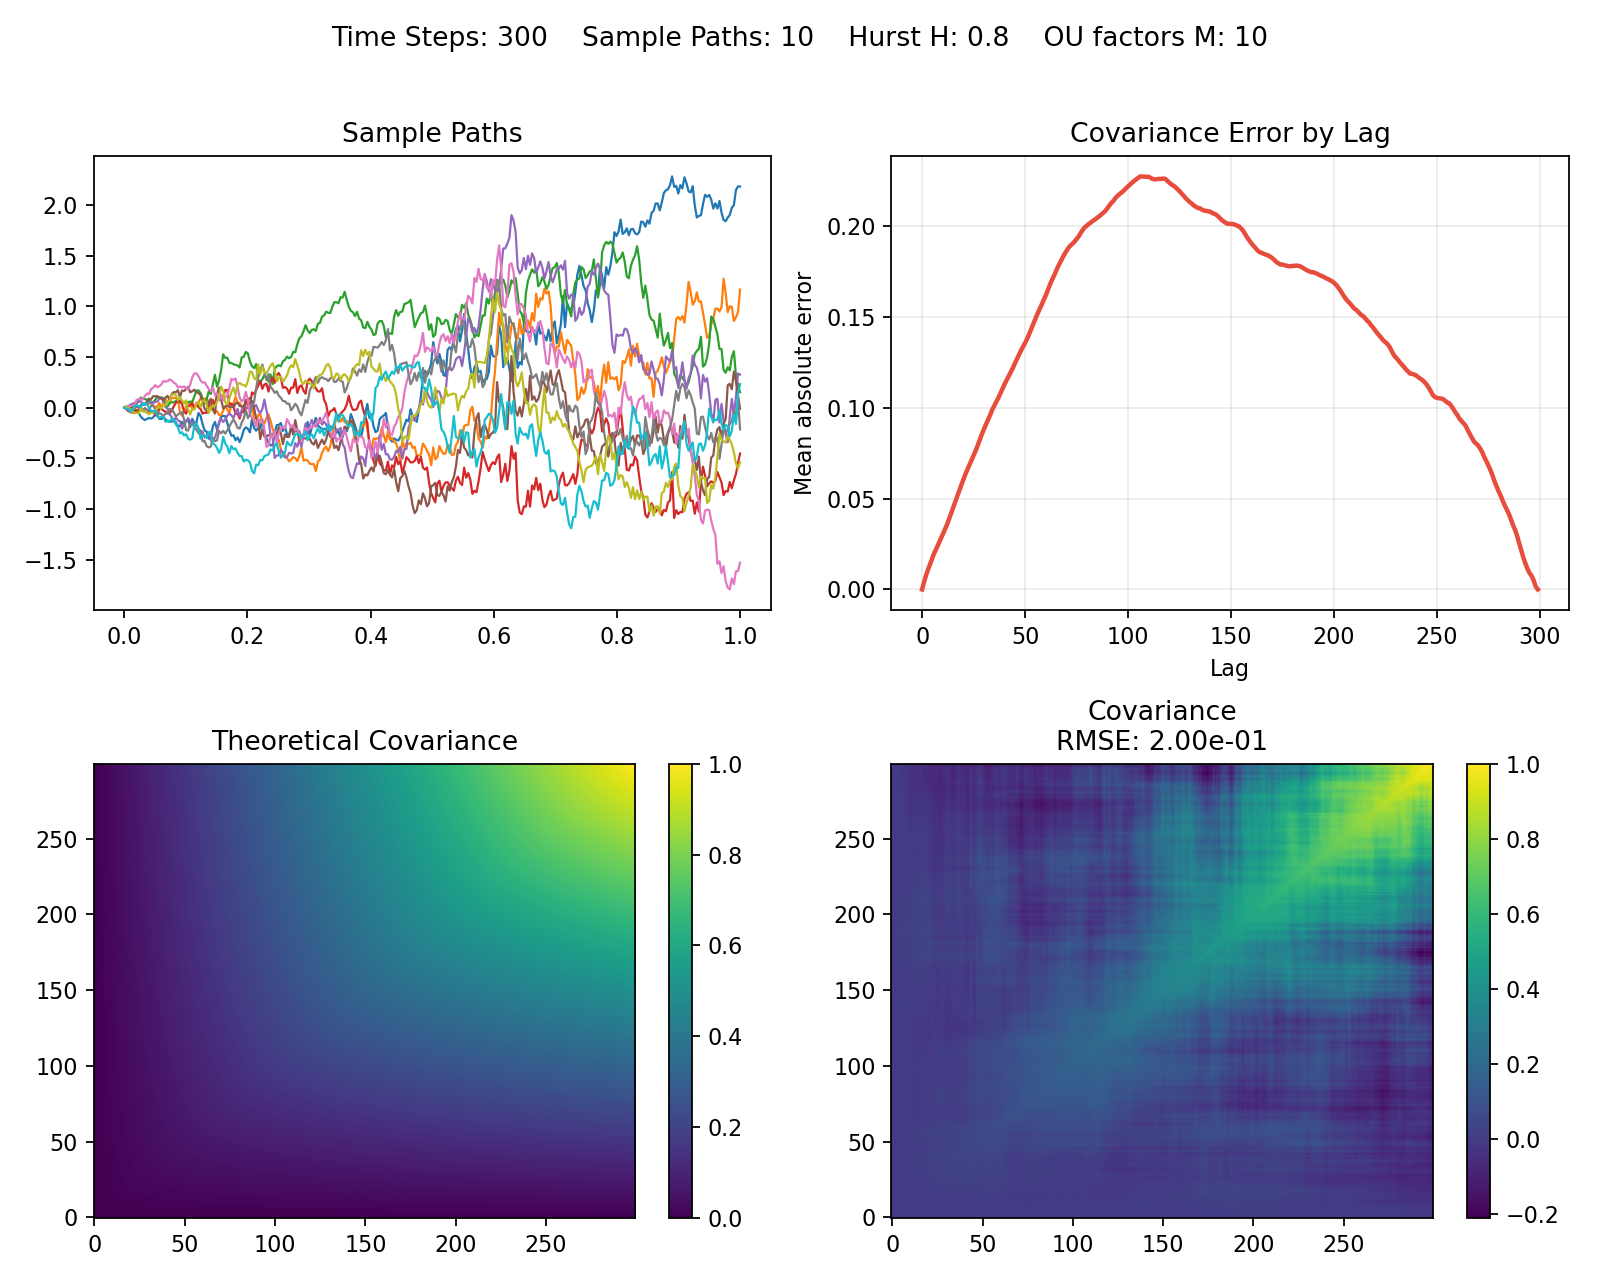
\includegraphics[width=6.5cm]{img/revisionato/2/ML0.8.png}
\end{minipage}
\end{figure}

\section{What lifting solves, and what it does not solve}

Markovian lifting does not make the process exactly equal to fractional Brownian motion at finite \(M\). That would be too strong a claim. What it does is much more practical: it replaces a non-Markovian singular-memory dynamics by a finite-dimensional Markov approximation that preserves the main covariance features sufficiently well for simulation and control.

This distinction matters. The purpose of lifting is not exact identity at fixed factor dimension, but tractability. The rough memory is compressed into a finite state vector,
\[
Z_t=\bigl(U_t^{(1)},\dots,U_t^{(M)}\bigr)^\top,
\]
and this state can be updated recursively. That is precisely what makes the method attractive for repeated Monte Carlo simulation, calibration to liquid instruments, and eventually inventory control inside a market-making engine.

From the perspective of the present paper, Markovian lifting is therefore the final step in the mathematical transition
\[
\text{fractional covariance}
\quad\longrightarrow\quad
\text{causal Volterra representation}
\quad\longrightarrow\quad
\text{finite-dimensional Markov state}.
\]
The next chapter uses this state-space perspective to reconnect the rough driver with a volatility process and, ultimately, with the reservation-price logic of a rough-volatility Avellaneda--Stoikov model.

\chapter{From Rough Paths to Rough Volatility}
\miniabstract{The previous chapters built the rough state in three layers: fractional covariance, causal Volterra dynamics, and finite-dimensional Markovian lifting. This chapter turns that state into a volatility input for the mid-price dynamics, so rough memory enters the price-risk forecast, the reservation price, and the quoting rule while also clarifying why the exact utility problem becomes harder.}

The modeling task is now operational. A lifted rough state must be embedded inside a positive volatility process without breaking the recursive simulation architecture, and the resulting variance forecast must be translated into an inventory-aware quoting rule.

\section{From a lifted rough state to a volatility factor}

Let
\[
Y_t^{(M)}=\sum_{k=1}^M w_k U_t^{(k)}
\]
denote the lifted Gaussian rough state obtained in the previous chapter, where the factors \(U^{(k)}\) satisfy OU-type dynamics. By construction, \(Y_t^{(M)}\) is Gaussian and can take both positive and negative values. For that reason, it should not be interpreted directly as a variance process. A separate link function is needed to map the rough state into a positive volatility or variance input.

There are two natural modeling routes.

The first is structural and closer to the rough-Heston literature. In that case one thinks of volatility as a Volterra-type process driven by a rough kernel, for example
\[
V_t
=
V_0
+
\int_0^t
K_\alpha(t-s)
\Bigl(
\kappa(\theta-V_s)\,ds
+
\xi\sqrt{V_s}\,dW_s^v
\Bigr),
\qquad
K_\alpha(\tau)=\frac{\tau^{\alpha-1}}{\Gamma(\alpha)},
\]
with \(\alpha=H+\tfrac12\in(\tfrac12,1)\). This specification is conceptually important because it shows how rough memory enters variance directly. However, for the present project it is not necessary to solve the full rough-Heston calibration problem in order to study market-making control.

The second route is more practical and better aligned with a simulation-first HFT study. One treats the lifted rough state as a latent Gaussian driver for log-volatility and defines, for example,
\[
\log v_t = m_t + \beta Y_t^{(M)},
\]
or equivalently
\[
v_t = \exp\!\bigl(m_t+\beta Y_t^{(M)}\bigr),
\]
where \(m_t\) is a deterministic baseline level and \(\beta>0\) controls the sensitivity of volatility to the rough factor. This choice guarantees positivity and preserves the intuition that large positive realizations of the rough state generate volatility clusters. It is also numerically convenient, because once the lifted factor has been simulated, the volatility process is obtained pointwise with no additional memory burden.

A slightly more stable centered version is
\[
v_t
=
\bar v\,
\exp\!\left(
\beta Y_t^{(M)}
-\frac12\beta^2\Var(Y_t^{(M)})
\right),
\]
which normalizes the unconditional level around \(\bar v\). The point is not that this is the only admissible specification, but that it turns the lifted state into a positive and simulation-ready volatility input.

\paragraph{Rough-volatility mid-price dynamics.}

Once a positive volatility process \(v_t\) has been constructed, the mid-price can be modeled by
\[
dS_t = \mu_t\,dt + \sqrt{v_t}\,dW_t^S,
\]
possibly with correlation between the price noise \(W^S\) and the volatility noise \(W^v\) or, in the lifted setting, between \(W^S\) and the Brownian driver behind the OU stack. At the level of the HFT engine, this is the natural rough-volatility replacement of the constant-\(\sigma\) benchmark studied in the first paper.

The interpretation is immediate. In the classical model, the dealer faces a fixed local price-risk scale. In the rough version, this local risk scale fluctuates over time and does so with memory. Volatility can remain elevated for a while, calm periods can cluster together, and the price-risk forecast now depends on the current state of the rough factor rather than on a single constant parameter.

This is precisely where the rough-state machinery becomes relevant for quoting. The dealer does not need roughness for its own sake; the dealer needs a state variable that updates the perceived risk of carrying inventory. Once \(v_t\) is stochastic and persistent, the inventory penalty should react accordingly.

\section{A rough variance forecast for quoting}

The natural quantity entering an inventory-aware quoting rule is not just the instantaneous variance \(v_t\), but the remaining integrated variance over the control horizon. Define the conditional variance forecast
\[
\widehat{\Sigma}_{t,T}^2
:=
\mathbb{E}_t\!\left[\int_t^T v_u\,du\right].
\]
In the classical finite-horizon benchmark with constant volatility, this reduces to
\[
\widehat{\Sigma}_{t,T}^2 = \sigma^2(T-t).
\]
In the rough setting, however, the same object becomes state dependent:
\[
\widehat{\Sigma}_{t,T}^2
=
\widehat{\Sigma}_{t,T}^2\bigl(Z_t\bigr),
\qquad
Z_t=\bigl(U_t^{(1)},\dots,U_t^{(M)}\bigr)^\top.
\]
This is the key conceptual bridge from the lifted model to inventory control. The state vector \(Z_t\) summarizes the relevant memory of the volatility driver, and from this state one computes the forecasted risk scale that replaces the constant \(\sigma^2(T-t)\) of the original Avellaneda--Stoikov benchmark.

A practical rough-volatility reservation price can then be written as
\[
r_t^{\mathrm{rough}}
=
S_t-\gamma q_t\,\widehat{\Sigma}_{t,T}^2,
\]
with a corresponding spread proxy
\[
\psi_t^{\mathrm{rough}}
=
\frac{2}{k}
+
\gamma\,\widehat{\Sigma}_{t,T}^2.
\]
This keeps the notation consistent with the first paper: \(S_t\) is the mid-price, \(q_t\) is inventory, \(\gamma\) is risk aversion, and \(k\) is the order-arrival sensitivity parameter. The only conceptual replacement is that the constant variance scale is upgraded to a state-dependent rough forecast. When \(v_t\equiv \sigma^2\), these formulas collapse back to the classical finite-horizon benchmark.

Hence the quoting rule becomes
\[
p_t^{ask}=r_t^{\mathrm{rough}}+\frac{\psi_t^{\mathrm{rough}}}{2},
\qquad
p_t^{bid}=r_t^{\mathrm{rough}}-\frac{\psi_t^{\mathrm{rough}}}{2}.
\]
This is not yet the exact optimal control for rough volatility, but it is the most natural extension of the classical inventory logic.

\section{Why the exact utility problem becomes difficult}

At this point one may ask whether the previous heuristic formulas can be justified directly from the same CARA-utility framework used in the classical Avellaneda--Stoikov model. Formally, the objective would still be
\[
\sup_{\pi}
\mathbb{E}\!\left[
-\exp\!\bigl(-\gamma(X_T+q_TS_T)\bigr)
\right],
\]
where \(\pi\) denotes the quoting policy. The problem is not the utility specification itself. Exponential utility remains a natural starting point because it preserves risk-aversion interpretability and fits well with marked-to-market wealth. The difficulty comes from the state dynamics.

Under rough volatility, the relevant Markov state is no longer just \((S_t,q_t)\), nor even \((S_t,q_t,v_t)\). Once lifting is introduced, the true state becomes
\[
(S_t,q_t,Z_t),
\qquad
Z_t\in\mathbb{R}^M.
\]
The value function is therefore of the form
\[
V(t,x,s,q,z)
=
\sup_{\pi}
\mathbb{E}_{t,x,s,q,z}
\!\left[
-\exp\!\bigl(-\gamma(X_T+q_TS_T)\bigr)
\right].
\]
Even though the lifted model is Markovian, it is Markovian in an enlarged state space of dimension \(M+3\) once cash is included. The corresponding HJB equation becomes substantially more complex than in the constant-volatility case.

Several specific difficulties arise.

First, the volatility process is now state dependent and persistent. This means that the continuation value depends not only on current inventory and current price, but also on the entire vector of lifted factors. The simple separation arguments used in the classical benchmark no longer go through cleanly.

Second, the arrival intensities and the price risk interact in a richer way. A dealer who sees a high-volatility rough state should generally quote more cautiously, but the best way to do so depends on how the execution intensities respond to the resulting spread changes. This turns the control problem into a coupled trade-off between inventory risk and fill risk in a higher-dimensional state space.

Third, if one allows correlation between the price Brownian motion and the volatility driver, the HJB acquires additional cross terms. Even when such correlation is ignored, the volatility forecast entering the value function is no longer deterministic.

Fourth, the exact optimal policy may not admit a closed-form expression. In the classical arithmetic Brownian benchmark, one obtains explicit or near-explicit reservation-price formulas because the value function retains a simple structure. Under rough volatility, even after lifting, there is no guarantee that the same exponential-affine ansatz will survive.

For these reasons, the utility problem remains well defined but analytically much less tractable. The lifting step restores Markovianity, not closed-form solvability.

\paragraph{Practical approximations to the control problem.}

The absence of a simple closed form does not make the model unusable. It only changes the level at which one works. Instead of insisting on a fully explicit optimal policy, one can proceed through structured approximations.

A first possibility is the \emph{frozen-state approximation}. One computes the conditional integrated variance forecast \(\widehat{\Sigma}_{t,T}^2\) from the current lifted state and plugs it into the classical reservation-price and spread formulas. This yields a quoting rule that is state dependent, causal, and easy to simulate.

A second possibility is simulation-based policy evaluation. One fixes a family of quoting rules parameterized by a small set of coefficients, simulates the marked-to-market utility under the rough-volatility engine, and then optimizes the coefficients numerically. In this approach, the lifted state is still essential because it allows recursive simulation without having to carry the full path.

A third possibility is to solve the HJB numerically on a reduced state grid, possibly after dimensionality reduction on the OU factors. This is more ambitious, but it is conceptually consistent with the lifted formulation.

The common theme is that the exact utility problem may lose analytical tractability, yet the lifted state keeps the model numerically accessible. This is precisely why the previous chapters were needed: without causality and without Markovian lifting, even these approximations would become cumbersome.

\section{Comparison with the naive benchmark from the first paper}

The most natural practical comparison for the present project is not against the exact rough-optimal policy, which may be unavailable in closed form, but against the same naive benchmark already used in the first paper. This keeps the notation, accounting, and execution logic fixed while changing only the volatility module.

In the naive symmetric policy, the dealer ignores both inventory and rough volatility and posts
\[
p_t^{bid,\mathrm{naive}} = S_t-\bar\delta,
\qquad
p_t^{ask,\mathrm{naive}} = S_t+\bar\delta,
\]
with \(\bar\delta\) constant or deterministic. This is the same baseline used in the classical article. It provides a clean benchmark because it separates spread capture from active risk control.

The rough inventory-aware policy preserves the same state variables but replaces the constant risk scale with the rough variance forecast:
\[
p_t^{bid,\mathrm{rough}} = r_t^{\mathrm{rough}}-\frac{\psi_t^{\mathrm{rough}}}{2},
\qquad
p_t^{ask,\mathrm{rough}} = r_t^{\mathrm{rough}}+\frac{\psi_t^{\mathrm{rough}}}{2}.
\]
Hence the comparison with the first paper is conceptually straightforward.

\begin{center}
\begin{tabularx}{\textwidth}{@{}lX@{}}
\toprule
Naive policy & Symmetric quotes around \(S_t\), no inventory correction, no rough-risk correction \\
Rough inventory-aware policy & Quotes centered around \(r_t^{\mathrm{rough}}\), with spread and skew driven by \(\widehat{\Sigma}_{t,T}^2(Z_t)\) \\
\bottomrule
\end{tabularx}
\end{center}

This comparison matters because rough volatility changes the environment in which the policy operates. In quiet periods, the naive policy may be overly conservative relative to the actual local risk. In clustered high-volatility periods, it may become too aggressive, keeping quotes too tight exactly when inventory is most dangerous. The rough-aware policy reacts to this state dependence by widening or skewing quotes according to the current volatility forecast.

The expected qualitative outcome is therefore the following. Relative to naive symmetric quoting, a rough-aware inventory rule should:
\begin{itemize}
    \item reduce inventory excursions when volatility clusters upward,
    \item stabilize marked-to-market wealth by reacting to persistent risk states,
    \item preserve more coherent quote behavior across regimes of calm and stress.
\end{itemize}
This is the rough-volatility analogue of the main lesson from the first paper. In the classical benchmark, inventory-aware quoting dominated naive quoting because it reacted to inventory. In the present rough setting, the natural extension is that quoting should react both to inventory and to the current memory-driven risk scale.

\paragraph{Role of this chapter in the overall project.}

The purpose of this chapter is not to claim that a full rough-volatility HJB has already been solved. Rather, it establishes the correct modeling bridge from the mathematical foundations to the market-making application. Chapters 2 through 4 explained how to build a rough state in a mathematically coherent and computationally causal way. The present chapter explains how that state enters the volatility process, how it modifies the reservation price, and why the exact utility problem becomes harder than in the classical benchmark.

This is enough to define the architecture of the second HFT project. The mid-price dynamics are upgraded from a constant-volatility diffusion to a rough-volatility diffusion; the reservation price is upgraded from a constant-variance inventory correction to a rough forecast correction; and the baseline comparison remains the same as in the first paper, namely naive symmetric quoting versus inventory-aware quoting. What changes is the risk engine behind the quotes.

In this sense, the present chapter is the operational hinge of the paper. The earlier chapters supplied the rough mathematical state. This chapter turns that state into a volatility module. The remainder of the paper can therefore focus on validation, implementation, and numerical comparison rather than on rebuilding the rough machinery from scratch.

\section{Implementation and validation workflow}

Three numerical layers are now available, and they should be treated as complementary rather than competing constructions.

\begin{center}
\begin{tabularx}{\textwidth}{@{}lX@{}}
\toprule
Method & Best use \\
\midrule
Direct covariance / Cholesky & Ground-truth benchmark for checking Gaussian covariance and marginal scaling \\
Causal Volterra discretization & Conceptual simulation of rough memory with explicit path dependence \\
Markovian lifting & Fast repeated simulation, state recursion, and control-oriented implementation \\
\bottomrule
\end{tabularx}
\end{center}

Before embedding the rough module inside a quoting engine, the following checks should be passed:
\begin{enumerate}[label=\arabic*.]
    \item \textbf{Marginal scaling:} verify numerically that \(\Var(X_t)\) follows the intended \(t^{2H}\)-type behavior.
    \item \textbf{Covariance structure:} compare empirical and theoretical covariance heatmaps on a fixed time grid.
    \item \textbf{Stability in \(n\):} refine the time grid and confirm that discretization error decreases.
    \item \textbf{Stability in paths:} increase the number of Monte Carlo paths and verify convergence of empirical moments.
    \item \textbf{State update consistency:} for the lifted model, confirm that the OU recursion reproduces the intended covariance shape as \(M\) increases.
\end{enumerate}

\paragraph{Research workflow for the HFT project.}

A coherent workflow for the project is then:
\begin{enumerate}[label=\arabic*.]
    \item validate the classical Avellaneda--Stoikov engine under standard diffusions;
    \item add a rough-volatility module and keep execution and accounting unchanged;
    \item impose end-of-day netting and a liquidation-aware terminal accounting rule;
    \item compare naive symmetric quoting with inventory-aware quoting under rough variance;
    \item stress test sensitivity to \(H\), horizon length, path count, liquidation parameters, and lift dimension \(M\).
\end{enumerate}

\begin{algorithm}[H]
\small
\caption{From rough driver to market-making simulation}
\DontPrintSemicolon
choose horizon \(T\), grid size \(n\), Hurst parameter \(H\), and lift dimension \(M\)\;
specify rates \(\lambda_k\), weights \(w_k\), inventory, cash, and mid-price initial values\;
\For{\(i=0,\dots,n-2\)}{
  update the lifted factors, aggregate \(Y_{i+1}=\sum_{k=1}^M w_k X_{i+1}^{(k)}\), and map it into variance\;
  update the mid-price, compute the inventory-aware quotes, sample executions, and update state variables\;
}
mark wealth to market, liquidate residual inventory when required, and record PnL diagnostics\;
\end{algorithm}

This closes the architecture and prepares the numerical chapter. The rough driver has now been defined, made causal, compressed into a lifted state, and translated into a volatility forecast. The remaining question is empirical: how does a policy using this state behave when inventory must be liquidated at the close?

\chapter{Numerical HJB with End-of-Day Netting}
\miniabstract{The previous chapter translated the lifted rough state into a volatility forecast and a rough-aware quoting rule. This final numerical experiment closes the loop by solving a reduced HJB calibrated to that state, simulating a full trading day with forced flat close, and comparing the resulting policy with a naive symmetric benchmark under anti-persistent, Brownian, and persistent Hurst regimes.}

The goal is to explain what changes once roughness enters the market-making environment, and why one should not read Avellaneda--Stoikov as a theorem about universal outperformance of every inventory-based strategy against every naive benchmark. The original result is an expected-utility statement under a Markovian price-and-execution model. If the traded mid-price itself were replaced by a fractional Brownian motion, the classical dynamic-programming argument would fail. For this reason the present experiment keeps the traded price conditionally diffusive and inserts roughness in the volatility state, where it can still be represented through Markovian lifting and then compressed into a tractable HJB state.

\section{Lift calibration across the three Hurst regimes}

The numerical comparison is run for
\[
H=0.2,\qquad H=0.5,\qquad H=0.8.
\]
In interpretive terms, these correspond respectively to an anti-persistent or locally mean-reverting-like regime, the standard Brownian benchmark, and a persistent or trend-following-like regime. The Markovian lifting uses the same six-factor grid in every case,
\[
M=6,
\qquad
\lambda=(3.0,\ 6.80,\ 15.43,\ 35.00,\ 79.37,\ 180.0),
\]
while the weights change with \(H\) through the power-law prescription
\[
w_k \propto \lambda_k^{-(H+1/2)}.
\]
As \(H\) increases, more weight shifts toward the slow factors. This is exactly what one should expect: the persistent regime keeps more memory in the low-frequency components, whereas the anti-persistent regime places relatively more mass on faster adjustments.

The full lift remains vector-valued, but the HJB is solved on a reduced scalar surrogate \(Y_t\). In the numerical implementation, the stationary variance of the lift is matched exactly, while the reduced mean-reversion scale used inside the HJB grid is kept common across the three runs at
\[
\kappa_Y=1.35.
\]
This is a deliberate modeling choice. It prevents the surface comparison from being dominated by the compression step itself, while still allowing \(H\) to alter the variance map and the persistence diagnostics of the lifted environment. The forward simulations, however, do \emph{not} collapse back to the same scalar OU path: they use the full lifted OU stack and only then aggregate it into the volatility driver. The induced local variance remains
\[
v_t
=
\sigma_0^2
\exp\!\left(
\beta Y_t
-\frac12\beta^2\Var(Y_\infty)
\right),
\]
with \(\sigma_0=1.1\) and \(\beta=0.75\), so that the traded mid-price follows
\[
dS_t=\sqrt{v_t}\,dW_t^S.
\]

Table~\ref{tab:hjb_calibration} summarizes the lift calibration. The monotone increase in \(\Var(Y_\infty)\) and in the lag-one autocorrelation makes the interpretation clear: the case \(H=0.2\) is the roughest and most reversal-prone, \(H=0.5\) is the benchmark, and \(H=0.8\) is the most persistent.

\begin{table}[H]
\centering
\caption{Markovian-lifting calibration used in the three numerical regimes. Common parameters across all runs are \(M=6\), \(\lambda \in [3,180]\), \(\kappa_Y=1.35\), \(A=14\), \(k=1.15\), \(\gamma=0.20\), and \(Q=6\).}
\label{tab:hjb_calibration}
\begin{tabular}{@{}lrrrrrr@{}}
\toprule
\(H\) & \(w_1\) & \(w_6\) & \(\Var(Y_\infty)\) & \(\rho_1\) & \(\eta_Y\) & Regime \\
\midrule
0.20 & 0.451 & 0.026 & 0.0776 & 0.9840 & 0.458 & Anti-persistent / mean-reverting-like \\
0.50 & 0.563 & 0.009 & 0.0983 & 0.9872 & 0.515 & Brownian benchmark \\
0.80 & 0.656 & 0.003 & 0.1147 & 0.9890 & 0.557 & Persistent / trend-following-like \\
\bottomrule
\end{tabular}
\end{table}

\section{HJB with terminal liquidation at the close}

The trading session covers a full day of \(390\) one-minute steps. Inventory is constrained to
\[
q_t\in\{-Q,\dots,Q\},
\]
and order arrivals keep the classical exponential form
\[
\lambda^b(\delta)=Ae^{-k\delta},
\qquad
\lambda^a(\delta)=Ae^{-k\delta},
\]
and the dealer is forced flat at the close. If \(q_{T^-}\) denotes the inventory held just before the market closes, then the liquidated terminal wealth is
\[
X_T^{\mathrm{liq}}
=
X_{T^-}+q_{T^-}S_T-L(q_{T^-},Y_T),
\qquad q_T=0.
\]
The liquidation penalty is
\[
L(q,y)=\bigl(c_0+c_1\sqrt{v(y)}\bigr)|q|+c_2q^2,
\]
with
\[
c_0=0.6,\qquad c_1=0.28,\qquad c_2=0.18.
\]
This is the key mechanism that makes end-of-day inventory economically relevant: carrying size into the close is not free, and it becomes especially expensive when local volatility is high.

The control objective is
\[
\sup_{\pi}\;\mathbb{E}\!\left[-\exp\!\bigl(-\gamma X_T^{\mathrm{liq}}\bigr)\right],
\]
and, using the usual CARA ansatz
\[
V(t,x,s,q,y)=-\exp\!\bigl(-\gamma(x+qs+\Theta(t,q,y))\bigr),
\]
the problem reduces to a semilinear HJB for \(\Theta\) with terminal condition
\[
\Theta(T,q,y)=-L(q,y).
\]
Because the arrival intensities remain exponential, the pointwise optimization in bid and ask offsets stays explicit:
\[
\delta_t^{b,*}
=
\frac{1}{\gamma}\ln\!\left(1+\frac{\gamma}{k}\right)
-\Bigl(\Theta(t,q+1,y)-\Theta(t,q,y)\Bigr),
\]
\[
\delta_t^{a,*}
=
\frac{1}{\gamma}\ln\!\left(1+\frac{\gamma}{k}\right)
-\Bigl(\Theta(t,q-1,y)-\Theta(t,q,y)\Bigr).
\]
The reservation-price mechanism is therefore unchanged in spirit, but the cost of carrying inventory is now state dependent because the risk scale is itself rough.

\section{Diagnostics, figures, and representative close-out paths}

The numerical pipeline produces the diagnostics and the two figures included below. Figure~\ref{fig:hjb_surfaces} reports the initial HJB surfaces for all three Hurst regimes. These panels are easy to misread on a first pass, so it is useful to separate the interpretation carefully.

\begin{algorithm}[H]
\caption{Reading the HJB surface figure}
\DontPrintSemicolon
\For{each \(H\in\{0.2,0.5,0.8\}\)}{
  calibrate the lifted rough environment and compress it to the HJB state \(y\)\;
  solve the reduced HJB backward on the \((q,y)\) grid with liquidation terminal condition\;
  export \(\Theta(0,q,y)\), \(\delta^{b,*}(0,q,y)\), and \(\delta^{a,*}(0,q,y)\)\;
}
read rows by regime and columns by continuation value, bid offset, and ask offset\;
\end{algorithm}

\begin{figure}[H]
\centering
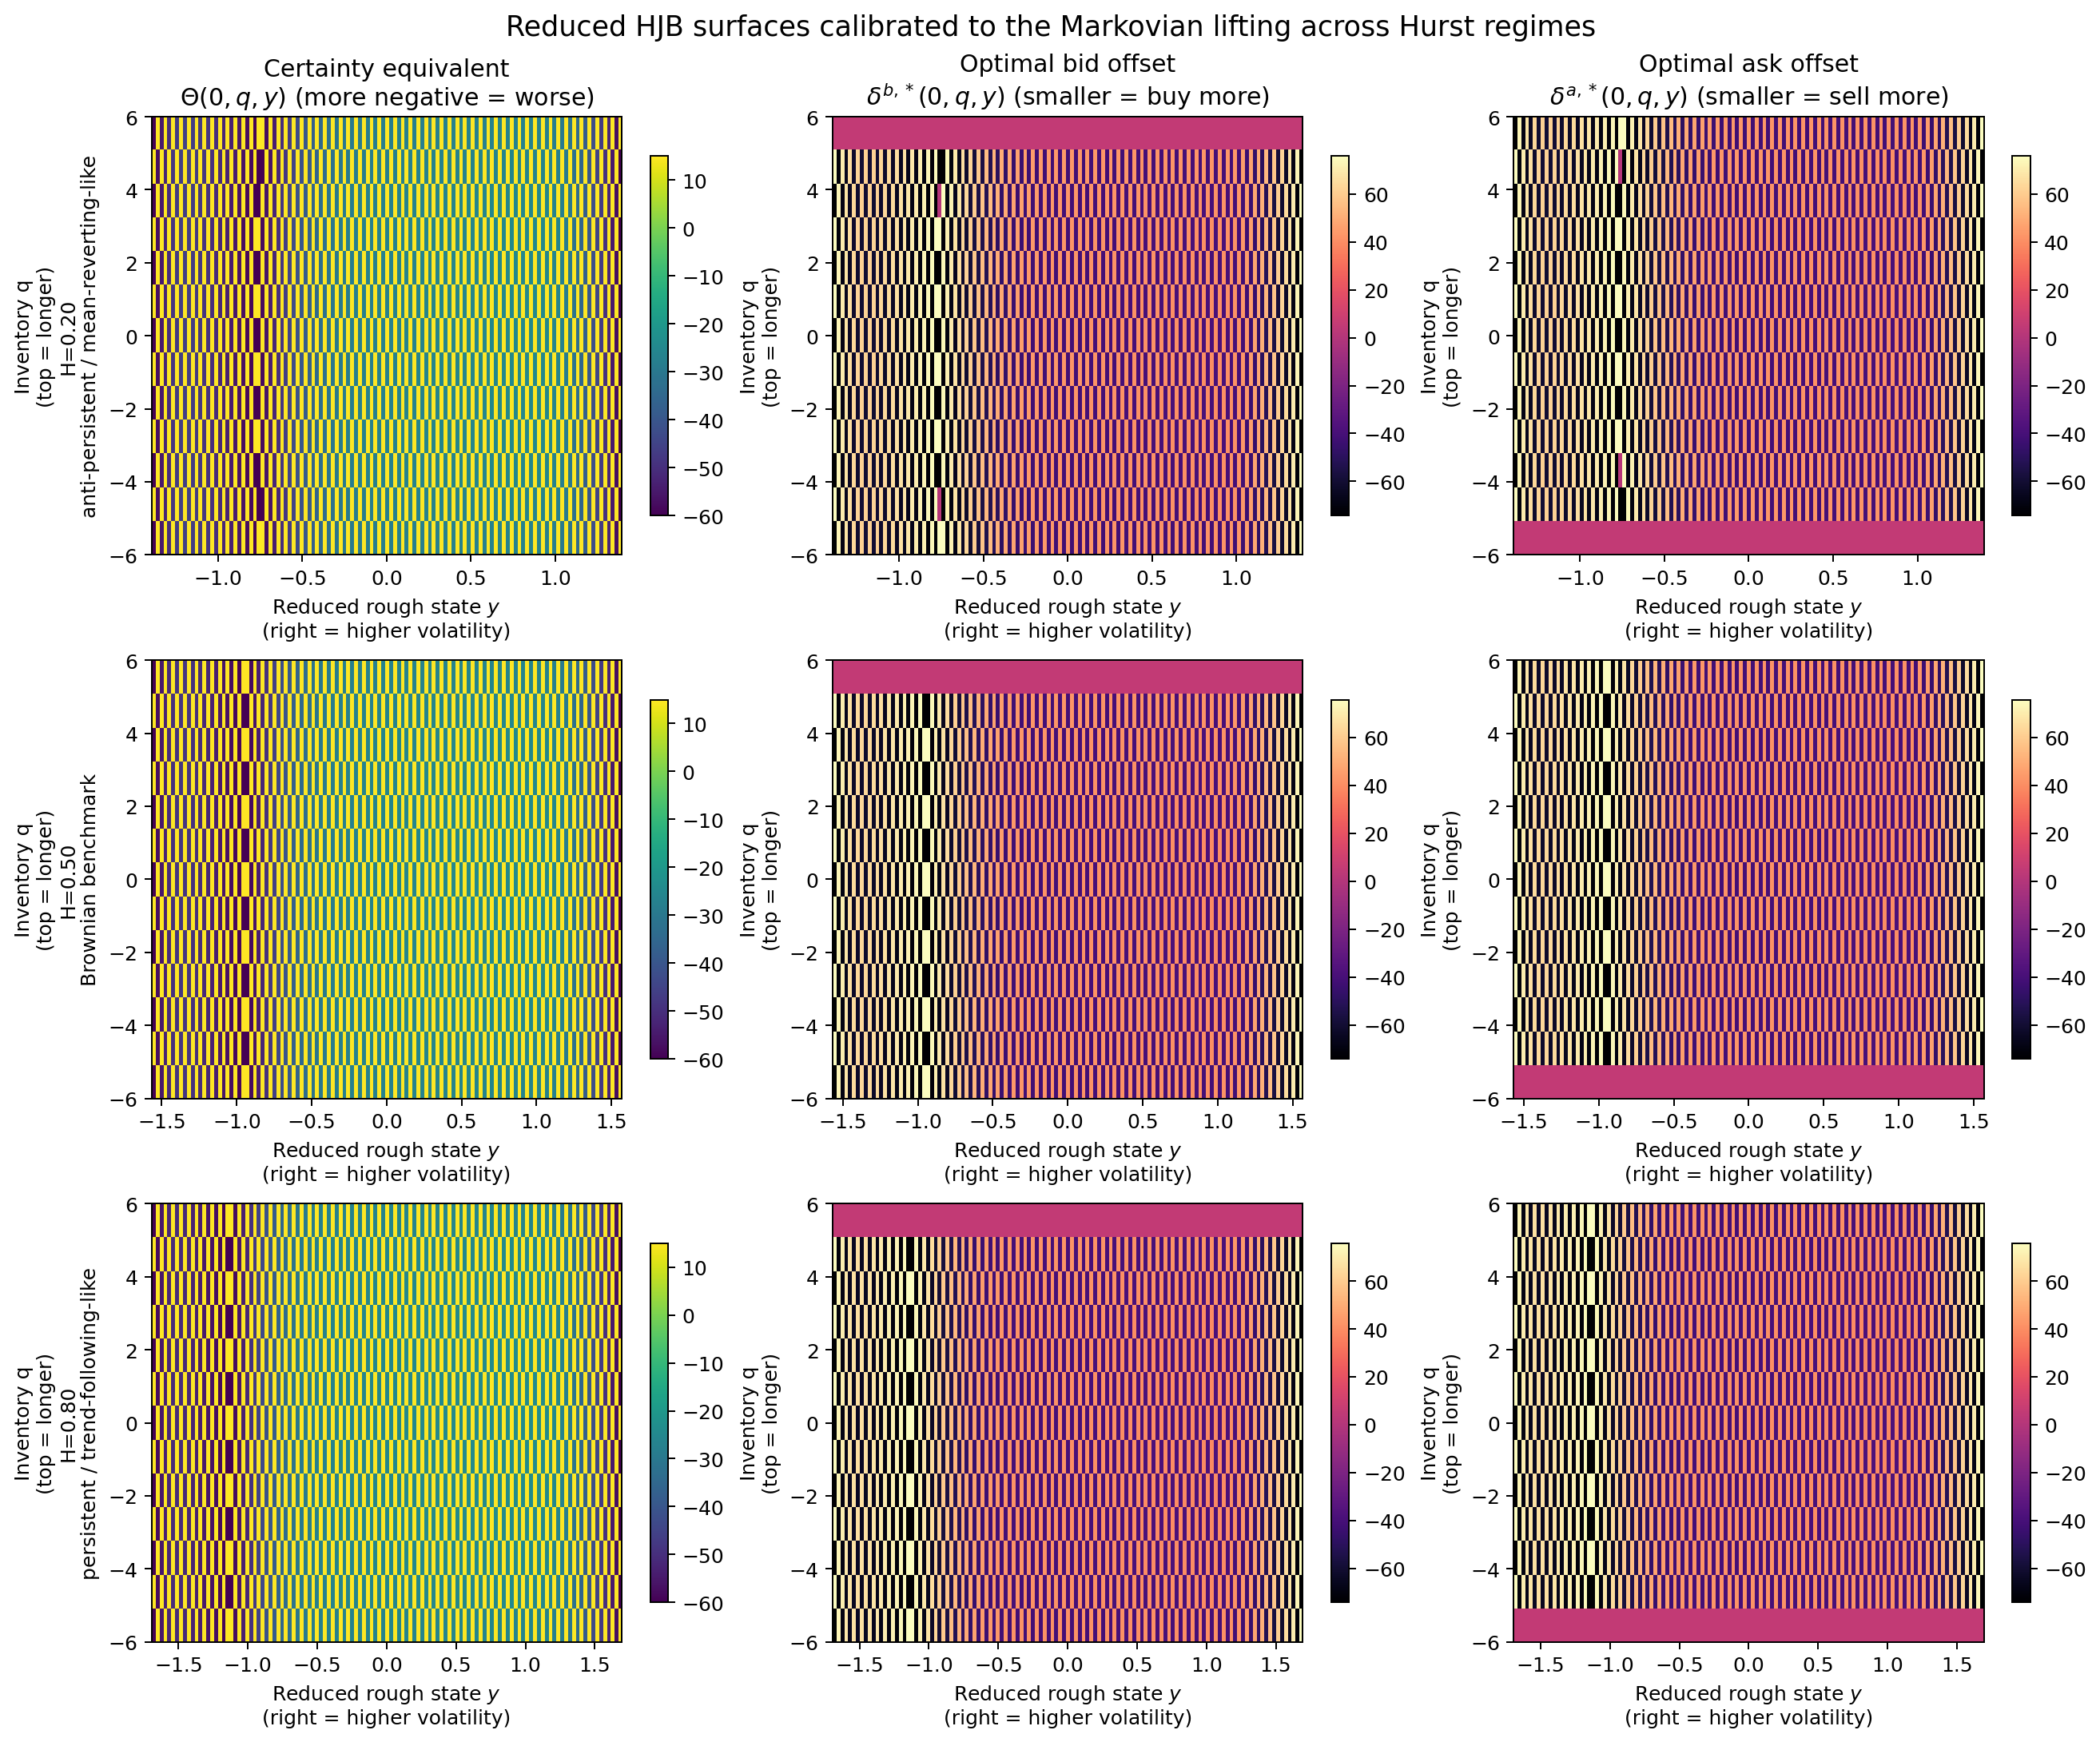
\includegraphics[width=\textwidth]{img/2/hjb_surfaces.png}
\caption{Reduced HJB surfaces across the three Hurst regimes. Each row corresponds to one lifted environment: \(H=0.2\) anti-persistent, \(H=0.5\) Brownian, and \(H=0.8\) persistent. The columns show the certainty-equivalent correction, the optimal bid offset, and the optimal ask offset at the initial time.}
\label{fig:hjb_surfaces}
\end{figure}

To read Figure~\ref{fig:hjb_surfaces}, fix one row first, so that \(H\) is held constant, and then move inside that row:
\begin{enumerate}[label=\arabic*.]
    \item The horizontal axis is the rough state \(y\). Moving to the right means a more stressed rough-volatility state and therefore a larger local variance forecast.
    \item The vertical axis is the inventory \(q\). Moving upward means the dealer is longer inventory; moving downward means the dealer is shorter inventory.
    \item In the first column, \(\Theta(0,q,y)\) is the continuation-value correction. More negative values mean that carrying that state forward is less attractive because future inventory risk and liquidation risk are more expensive.
    \item In the second column, \(\delta^{b,*}(0,q,y)\) is the optimal bid offset. A \emph{smaller} bid offset means the bid is closer to the mid-price, so the dealer buys more aggressively. A \emph{larger} bid offset means the dealer backs the bid away and becomes less willing to buy.
    \item In the third column, \(\delta^{a,*}(0,q,y)\) is the optimal ask offset. A \emph{smaller} ask offset means the ask is closer to the mid-price, so the dealer sells more aggressively. A \emph{larger} ask offset means the dealer is less willing to sell.
\end{enumerate}

The Avellaneda--Stoikov asymmetry is therefore read vertically. If one moves upward to positive inventory, the dealer should buy less aggressively and sell more aggressively: the bid offset widens, the ask offset tightens, and the certainty-equivalent surface deteriorates. If one moves downward to negative inventory, the pattern reverses. The effect of the rough state is read horizontally: moving toward larger \(y\) raises the volatility forecast, so both quotes tend to become more conservative overall, while the exact curvature changes across the three Hurst regimes.

The volatility diagnostics confirm that the environment remains genuinely stochastic in all three cases. The mean integrated variance changes only slightly, but the dispersion increases with \(H\), which is consistent with the fact that persistent regimes keep variance excursions alive for longer. This is why it is useful to report not only PnL and inventory, but also volatility statistics themselves.

\begin{table}[H]
\centering
\caption{Volatility diagnostics of the simulated environment across \(2{,}000\) trading days.}
\label{tab:hjb_vol_diagnostics}
\begin{tabular}{@{}lrrrr@{}}
\toprule
\(H\) & Mean realized vol & Std realized vol & Mean integrated var & Std integrated var \\
\midrule
0.20 & 1.096 & 0.081 & 1.209 & 0.155 \\
0.50 & 1.095 & 0.090 & 1.209 & 0.180 \\
0.80 & 1.095 & 0.098 & 1.208 & 0.199 \\
\bottomrule
\end{tabular}
\end{table}

Figure~\ref{fig:hjb_simulation} then collects one representative day for each regime. The left column shows the lifted rough state together with the induced local variance, the center column shows the inventory path from the open to the forced flat close, and the right column compares the end-of-day liquidated PnL distributions of the naive and HJB strategies. The main pattern is robust across all three regimes: the HJB policy consistently keeps much less inventory into the close, which translates into a much smaller liquidation bill.

\begin{algorithm}[H]
\caption{Reading the close-out simulation figure}
\DontPrintSemicolon
\For{each simulated trading day}{
  update the lifted rough state and map it into local variance\;
  simulate the mid-price and order arrivals under common random numbers\;
  compare naive symmetric quoting with the HJB inventory-aware policy\;
  force terminal liquidation, record close-out cost, PnL, and inventory diagnostics\;
}
select one representative path per regime and plot it beside the Monte Carlo PnL histograms\;
\end{algorithm}

The representative path is now selected separately inside each regime, which is the natural choice once the forward simulation uses the full lifted state and the three Hurst cases no longer share the same effective trajectory. Table~\ref{tab:hjb_representative_path} makes the close-out mechanics explicit. In every regime the HJB policy still arrives at the close with materially smaller inventory and therefore a much smaller liquidation bill than the naive benchmark.

\begin{table}[H]
\centering
\caption{Representative regime-specific paths from Figure~\ref{fig:hjb_simulation}.}
\label{tab:hjb_representative_path}
\begin{tabular}{@{}lrrrrrrr@{}}
\toprule
\(H\) & Seed & \(q_{T^-}^{\mathrm{naive}}\) & \(q_{T^-}^{\mathrm{HJB}}\) & \(L^{\mathrm{naive}}\) & \(L^{\mathrm{HJB}}\) & PnL\(_{\mathrm{naive}}\) & PnL\(_{\mathrm{HJB}}\) \\
\midrule
0.20 & 218 & 4.000 & -1.000 & 6.290 & 1.032 & -1.349 & 2.533 \\
0.50 & 250 & 4.000 & 1.000 & 6.719 & 1.140 & 5.544 & 8.833 \\
0.80 & 235 & 6.000 & 2.000 & 11.816 & 2.499 & 1.087 & 2.886 \\
\bottomrule
\end{tabular}
\end{table}

\begin{figure}[H]
\centering
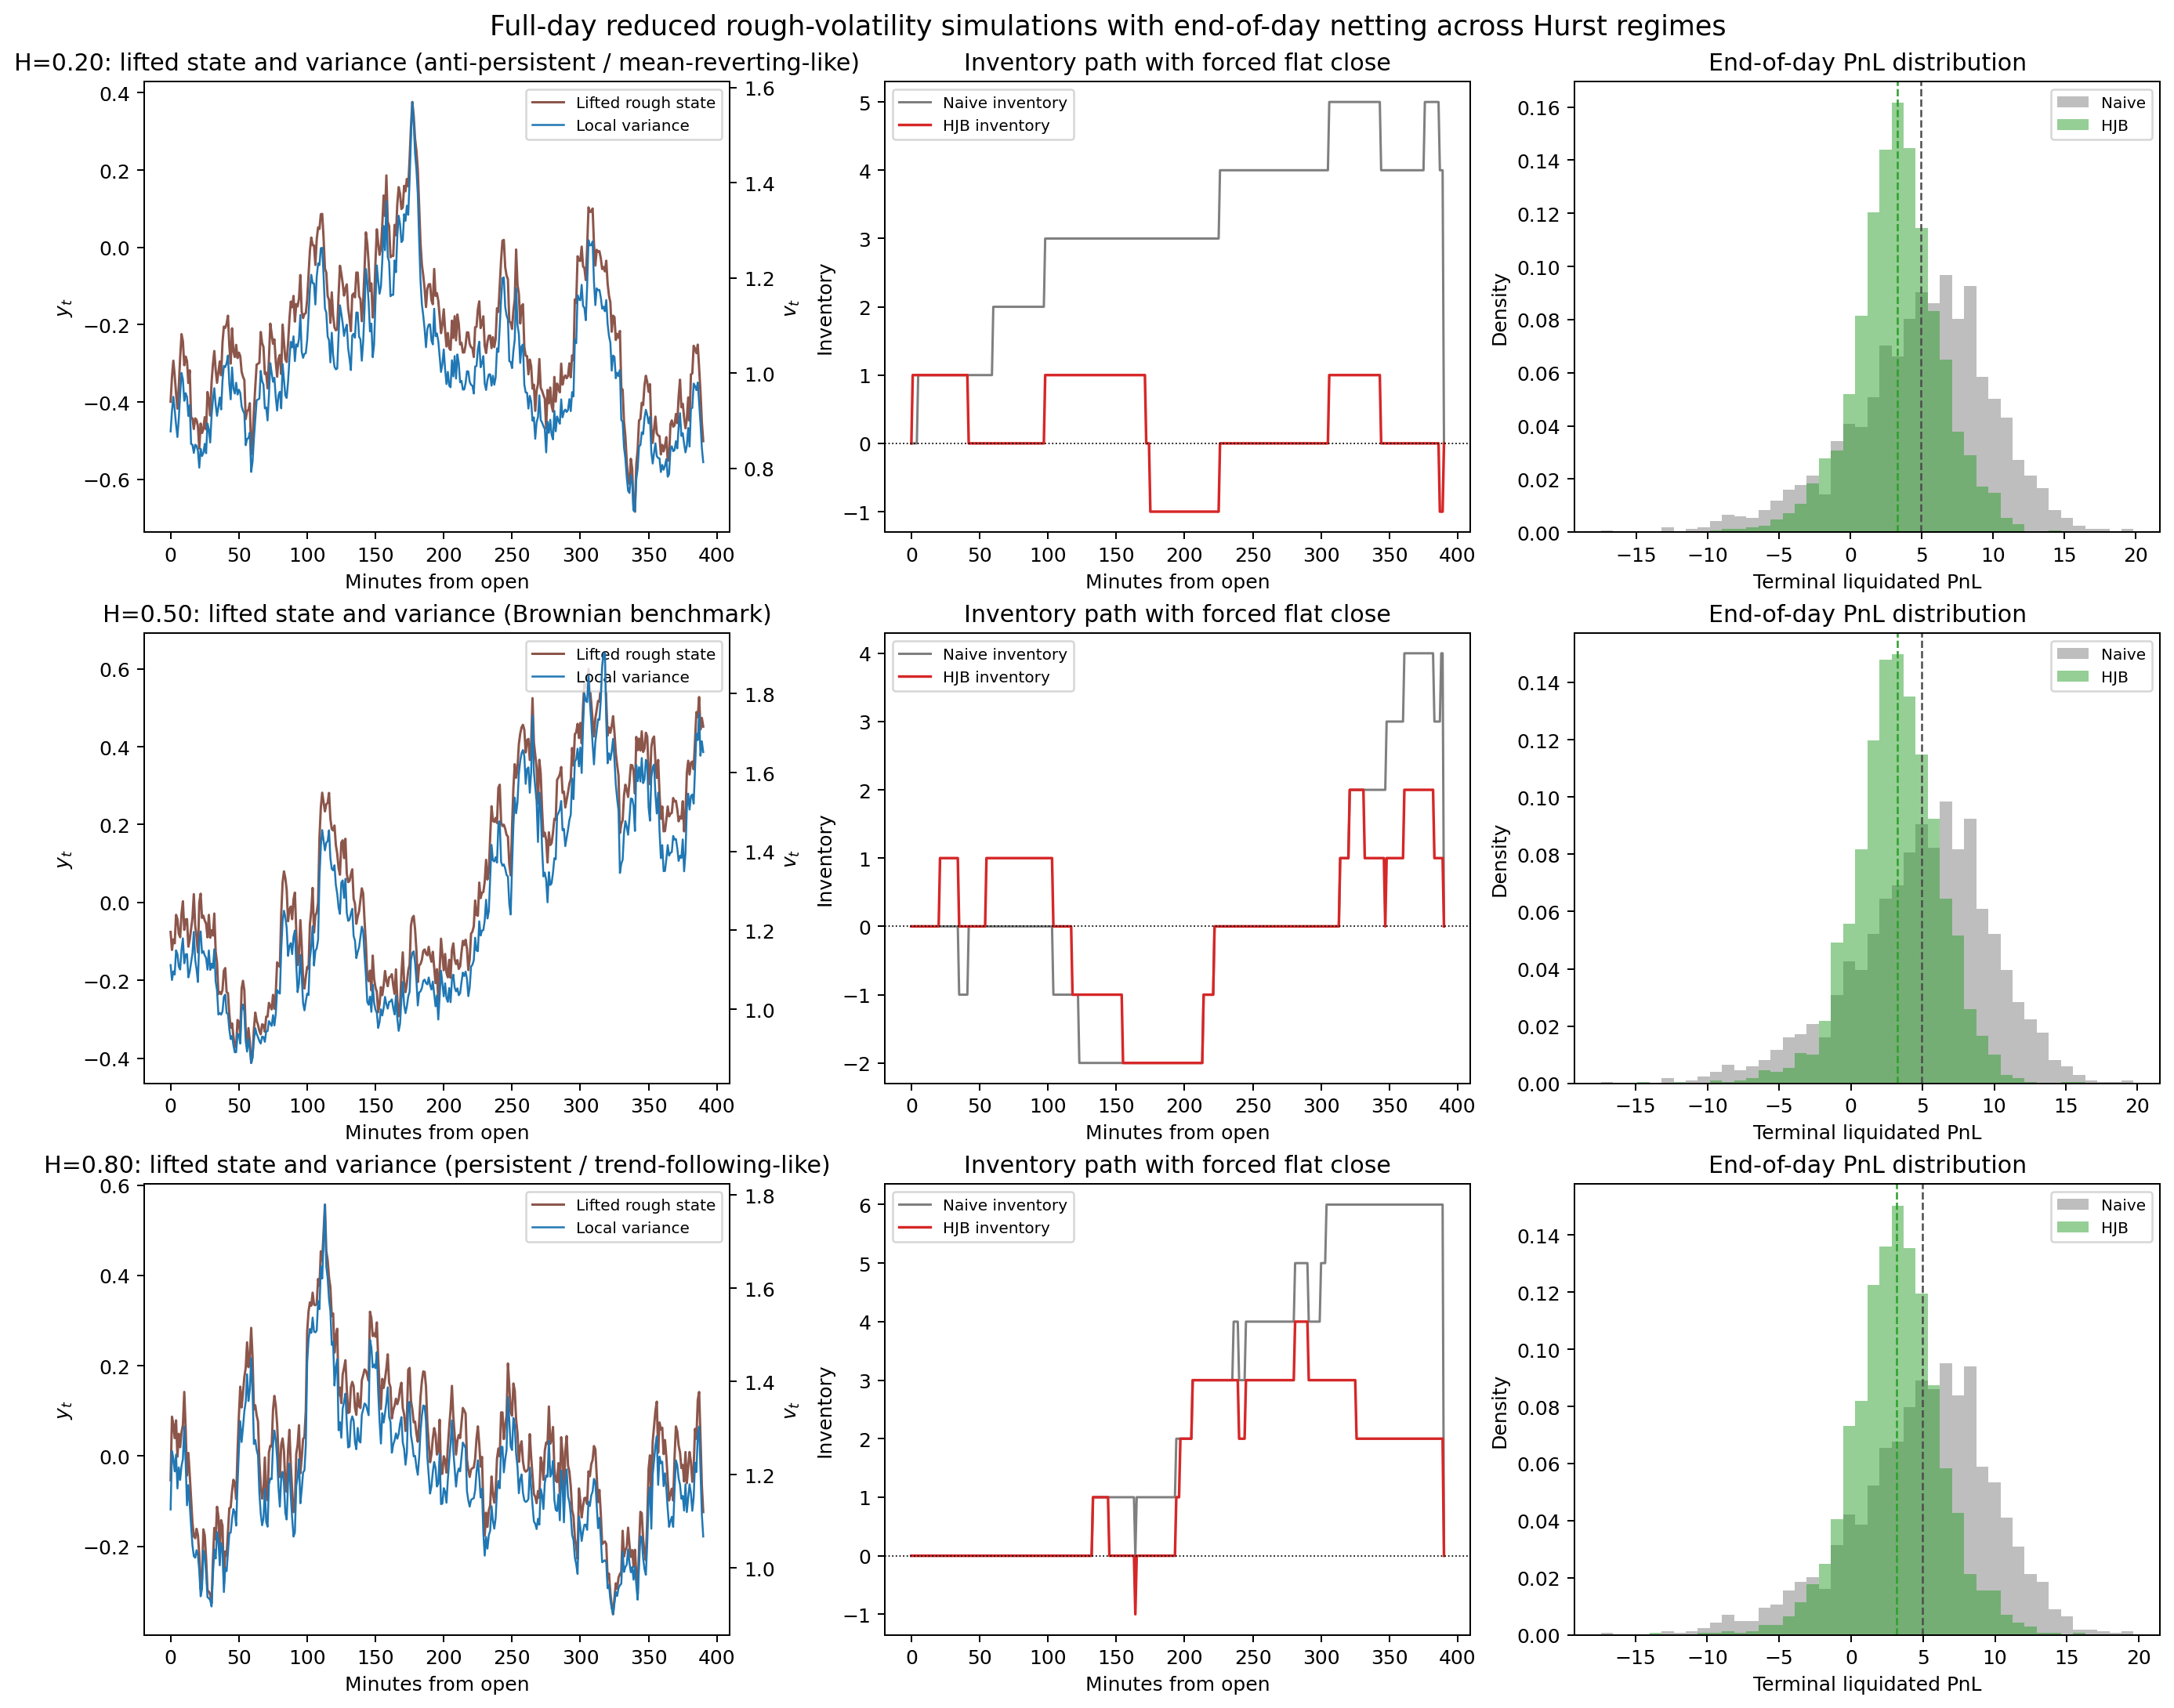
\includegraphics[width=\textwidth]{img/2/hjb_simulation.png}
\caption{Representative full-day simulations and Monte Carlo histograms across the three Hurst regimes. Rows correspond to \(H=0.2\), \(H=0.5\), and \(H=0.8\); columns show the lifted rough state and local variance, the inventory path with forced flat close, and the end-of-day liquidated PnL distribution.}
\label{fig:hjb_simulation}
\end{figure}

\section{Monte Carlo evidence and interpretation}

The full Monte Carlo comparison is reported in Tables~\ref{tab:hjb_mc_risk} and \ref{tab:hjb_mc_inventory}. Several points are worth separating carefully.

First, the naive benchmark keeps the larger \emph{mean} PnL in every regime. This is not a contradiction of Avellaneda--Stoikov. A symmetric spread-capture strategy can earn more average PnL precisely because it is willing to warehouse inventory and postpone the risk accounting until the close. The relevant question is therefore not ``which policy has the largest raw mean PnL?'', but rather ``what happens after one charges the close-out risk consistently?''

Second, on the dimensions that measure end-of-day inventory risk directly, the HJB is uniformly better. In all three regimes the average pre-close inventory falls from about \(2.50\) to roughly \(0.55\), and the average liquidation cost falls from about \(3.99\) to roughly \(0.67\). The left tail also improves materially: the 5\% expected shortfall is less negative in every case.

\begin{table}[H]
\centering
\caption{Risk-adjusted Monte Carlo comparison with forced net-zero close (\(2{,}000\) sessions).}
\label{tab:hjb_mc_risk}
\begin{tabular}{@{}lrrrrrr@{}}
\toprule
\(H\) & Sharpe\(_N\) & Sharpe\(_H\) & CE\(_N\) & CE\(_H\) & ES\(_N\) & ES\(_H\) \\
\midrule
0.20 & 1.017 & 1.110 & 2.052 & 2.352 & -6.870 & -3.607 \\
0.50 & 1.017 & 1.082 & 2.056 & 2.208 & -6.865 & -3.734 \\
0.80 & 1.018 & 1.034 & 2.059 & 2.156 & -6.862 & -3.681 \\
\bottomrule
\end{tabular}
\end{table}

\begin{table}[H]
\centering
\caption{Inventory and liquidation metrics across the three Hurst regimes.}
\label{tab:hjb_mc_inventory}
\begin{tabular}{@{}lrrrrrr@{}}
\toprule
\(H\) & Mean PnL\(_N\) & Mean PnL\(_H\) & \(\E|q_{T^-}|_N\) & \(\E|q_{T^-}|_H\) & \(\E L_N\) & \(\E L_H\) \\
\midrule
0.20 & 4.955 & 3.309 & 2.504 & 0.547 & 3.990 & 0.654 \\
0.50 & 4.957 & 3.244 & 2.504 & 0.572 & 3.989 & 0.693 \\
0.80 & 4.958 & 3.173 & 2.504 & 0.549 & 3.988 & 0.667 \\
\bottomrule
\end{tabular}
\end{table}

The interpretation of the three regimes is now cleaner than before. For \(H=0.2\), the anti-persistent rough driver is the most favorable case for the HJB: the strategy gives up some mean PnL, but it improves Sharpe, certainty equivalent, and tail risk while dramatically shrinking the liquidation bill. For \(H=0.5\), the Brownian benchmark still leaves more raw spread-capture income to the naive policy, yet the HJB remains clearly superior on Sharpe, certainty equivalent, inventory discipline, and close-out cost. For \(H=0.8\), the persistent regime remains the hardest case in the sense that the risk-adjusted gain becomes smaller, but even there the HJB still improves Sharpe, improves certainty equivalent, improves expected shortfall, and cuts liquidation cost by a large margin.

This is precisely where the earlier conceptual discussion matters. Avellaneda--Stoikov proves optimality for a Markovian utility-maximization problem, not universal dominance in raw mean PnL after one changes the environment and adds forced end-of-day liquidation. In the present implementation, the naive benchmark still wins on average PnL because it warehouses inventory more aggressively. The HJB, however, dominates on the dimensions that actually price inventory risk correctly at the close.

The practical conclusion is therefore sharper. If one optimizes only raw mean PnL, the naive benchmark can still look attractive because it monetizes spread capture by tolerating much larger end-of-day inventory. Once one cares about close-out discipline, liquidation cost, certainty equivalent, and left-tail protection, the inventory-aware HJB is preferable in all three regimes.

The numerical evidence therefore gives the paper its final bridge. The first chapters built the rough-volatility state; this chapter showed how that state changes the quoting problem when liquidation is priced explicitly. The conclusion can now summarize the whole path from fractional covariance to an implementable end-of-day inventory rule.

\chapter*{Conclusion}
\addcontentsline{toc}{chapter}{Conclusion}
\markboth{Conclusion}{Conclusion}

The mathematical route developed in this article is now complete. Fractional Brownian motion introduced the covariance structure of memory and the role of the Hurst parameter. Volterra representations then translated that global covariance picture into a causal construction that is compatible with sequential simulation. Markovian lifting finally provided the computational bridge from singular memory kernels to a finite-dimensional state that can be filtered, simulated, and embedded inside a control problem.

The last chapter showed why this route matters operationally. The roughness should not be placed directly in the traded mid-price if one wants to remain close to the dynamic-programming logic of Avellaneda--Stoikov. The correct compromise is to keep the mid-price conditionally diffusive, place roughness in the volatility state, and solve the HJB on a tractable surrogate calibrated to the lift. This is exactly what was implemented in the numerical experiments, whose tables, figures, and Monte Carlo diagnostics are included in the text.

The three-case comparison \(H=0.2,0.5,0.8\) also sharpens the economic interpretation. The anti-persistent case is the clearest victory for the inventory-aware policy, because the gain in risk-adjusted performance is the strongest there. The Brownian benchmark remains favorable to the HJB once one prices liquidation and tail risk correctly. The persistent case is still the most demanding one, since the improvement over the naive benchmark becomes smaller, but the HJB continues to dominate on Sharpe, certainty equivalent, and close-out discipline. This is not a failure of the original Avellaneda--Stoikov idea. It is evidence that, once rough persistence is introduced, the quality of the state compression remains part of the model risk even when the overall policy comparison still favors the HJB.

In this sense, the article closes the full logical circle without pretending that the final implementation is already the last word. Fractional covariance provided the language of memory, Volterra dynamics supplied causality, lifting restored a finite-dimensional state, and the numerical HJB turned that state into an actual quoting policy with end-of-day netting. The natural continuation of Article~2 is therefore clear: richer reduced-state calibrations, execution models that react to persistent regimes more explicitly, and liquidation-aware controls that preserve the discipline of ending the day flat without sacrificing too much spread-capture capacity when persistence becomes dominant.


\begin{references}
\bibitem{AvellanedaStoikov2008}
Marco Avellaneda and Sasha Stoikov,
\emph{High-frequency trading in a limit order book},
\emph{Quantitative Finance} 8(3), 217--224, 2008.

\bibitem{BayerFrizGatheral2016}
Christian Bayer, Peter Friz, and Jim Gatheral,
\emph{Pricing under rough volatility},
\emph{Quantitative Finance} 16(6), 887--904, 2016.

\bibitem{ElEuchRosenbaum2019}
Omar El Euch and Mathieu Rosenbaum,
\emph{The rough Heston model},
\emph{Mathematical Finance} 29(1), 3--38, 2019.

\bibitem{GatheralJaissonRosenbaum2018}
Jim Gatheral, Thibault Jaisson, and Mathieu Rosenbaum,
\emph{Volatility is rough},
\emph{Quantitative Finance} 18(6), 933--949, 2018.

\bibitem{MandelbrotVanNess1968}
Benoit B. Mandelbrot and John W. Van Ness,
\emph{Fractional Brownian motions, fractional noises and applications},
\emph{SIAM Review} 10(4), 422--437, 1968.

\bibitem{Gueant2017}
Olivier Gu\'eant,
\emph{The Financial Mathematics of Market Liquidity: From Optimal Execution to Market Making},
CRC Press, 2017.
\bibitem{HFT2Code}
Salvatore Gabriele Messina and Niccol\`o Soriano,
\emph{Rough Volatility and End-of-Day Inventory Control: supporting code},
Starting Finance Club PoliTo, GitHub repository,
\url{https://github.com/StartingFinanceClubPoliTo/Research/tree/main/Stoikov-Avellonada/Article-2-Rough-Volatility-HJB},
accessed 26/06/2026.
\end{references}

\end{document}
